%%%%%%%%%%%%%%%%%%%%%%%%%%%%%%%%%%%%%%%%%%%%%%%%%%%%%%%%%%%%%%%%%%%%%%
%%  disstemplate.tex, to be compiled with latex.         %
%%  08 April 2002 Version 4            %
%%%%%%%%%%%%%%%%%%%%%%%%%%%%%%%%%%%%%%%%%%%%%%%%%%%%%%%%%%%%%%%%%%%%%%
%%                     %
%%  Writing a Doctoral Dissertation with LaTeX at        %
%%  the University of Texas at Austin          %
%%                     %
%%  (Modify this ``template'' for your own dissertation.)      %
%%                     %
%%%%%%%%%%%%%%%%%%%%%%%%%%%%%%%%%%%%%%%%%%%%%%%%%%%%%%%%%%%%%%%%%%%%%%


\documentclass[12pt]{report}  % The documentclass must be ``report''.

\usepackage{utdiss2}      % Dissertation package style file.


%%%%%%%%%%%%%%%%%%%%%%%%%%%%%%%%%%%%%%%%%%%%%%%%%%%%%%%%%%%%%%%%%%%%%%
% Optional packages used for this sample dissertation. If you don't  %
% need a capability in your dissertation, feel free to comment out   %
% the package usage command.               %
%%%%%%%%%%%%%%%%%%%%%%%%%%%%%%%%%%%%%%%%%%%%%%%%%%%%%%%%%%%%%%%%%%%%%%
\usepackage[lined,linesnumbered,boxed,oldcommands]{algorithm2e}
\usepackage{subfigure}
\usepackage{multirow}
\usepackage{cancel}
\usepackage{color}
\usepackage{amsmath,amssymb,amsthm,amsfonts,amscd} 
        % Some packages to write mathematics.
\usepackage{eucal}    % Euler fonts
\usepackage{verbatim}       % Allows quoting source with commands.
\usepackage{makeidx}        % Package to make an index.
%% %%\usepackage{psfig}           % Allows inclusion of eps files.
\usepackage{epsfig}           % Allows inclusion of eps files.
%% \usepackage{citesort}          
\usepackage{url}
\usepackage[hyperindex]{hyperref}     % Allows good typesetting of web URLs.
\usepackage{xspace}
\usepackage{booktabs}
\usepackage{caption}
\usepackage{pbox}

\newcommand{\etal}{{\em et al.}}

\newlength{\figurewidthA} % 1 figure in a row (1 column)
\setlength{\figurewidthA}{0.49\columnwidth}

\newlength{\figurewidthB} % 2 figures in a row (1 column)
\setlength{\figurewidthB}{0.485\columnwidth}

\newlength{\figurewidthC} % adjust sizes of figures to save space
\setlength{\figurewidthC}{0.65\columnwidth}

\newlength{\figurewidthE} % 3 figures in a row (2 columns)
\setlength{\figurewidthE}{0.33\columnwidth}

\newlength{\figurewidthF} % 4 figures in a row (2 columns)
\setlength{\figurewidthF}{1.5in} %#0.5\columnwidth}


\newlength{\figurewidthG} % 2 figures in a row (1 column)
\setlength{\figurewidthG}{0.45\columnwidth}

\newlength{\figurewidthH} % 3 figures in a row (2 columns)
\setlength{\figurewidthH}{0.38\columnwidth}

\newlength{\figurewidthI} % 3 figures in a row (2 columns)
\setlength{\figurewidthI}{0.31\columnwidth}

\newcommand{\pname}[0]{$DA^2$}


\newcommand{\naive}{na\"{\i}ve}

\newcommand{\En}{\mathsf{E}}
\newcommand{\Dc}{\mathsf{D}}
\newcommand{\VK}{V\!K}
%%%%%%%%% GET SOME SPACE BY CHANGING THE ENVIRONMENT %%%%%%%%%%%%%%%%%%%%%%%%
\newenvironment{sitemize}{%
  \begin{list}{$\bullet$}{%
    %\setlength{\rightmargin}{\leftmargin}
    \setlength{\itemsep}{0.2cm}%
    \setlength{\leftmargin}{1.5em}%
    \setlength{\topsep}{4pt plus 2pt minus 2pt}%
    \setlength{\parsep}{0.0cm}}%
  }{\end{list}}

\newenvironment{senumerate}{%
   \begin{list}{\arabic{enumi}.}{%
    \setlength\labelwidth{1.5em}%
    \setlength\leftmargin{1.5em}%
    \setlength{\topsep}{4pt plus 2pt minus 2pt}%
    \setlength\itemsep{0.0cm}%
    \usecounter{enumi}}%
  }{\end{list}}

\newcommand{\defas}{\ensuremath{\stackrel{\scriptscriptstyle{\triangle}}{=}}}

%%%%%%%%%%%%%%%%%% FORMATTING ALGORITHMS %%%%%%%%%%%%%%%%%%%%%%%%%%%%%%%%%%%%%




%% %%\usepackage{draftcopy}   % Uncomment this line to have the
%%        % word, "DRAFT," as a background
%%        % "watermark" on all of the pages of
%%        % of your draft versions. When ready
%%        % to generate your final copy, re-comment
%%        % it out with a percent sign to remove
%%        % the word draft before you re-run
%%        % Makediss for the last time.

\author{Yi-Chao Chen}   % Required

\address{3517 North Hills Dr, Apt DD201,\\ Austin, Texas 78731}  % Required

\title{Robust Network Compressive Sensing}
                                                    % Required

%%%%%%%%%%%%%%%%%%%%%%%%%%%%%%%%%%%%%%%%%%%%%%%%%%%%%%%%%%%%%%%%%%%%%%
% NOTICE: The total number of supervisors and other members %%%%%%%%%%
%%%%%%%%%%%%%%% MUST be seven (7) or less! If you put in more, %%%%%%%
%%%%%%%%%%%%%%% they are put on the page after the Committee %%%%%%%%%
%%%%%%%%%%%%%%% Certification of Approved Version page. %%%%%%%%%%%%%%
%%%%%%%%%%%%%%%%%%%%%%%%%%%%%%%%%%%%%%%%%%%%%%%%%%%%%%%%%%%%%%%%%%%%%%

%%%%%%%%%%%%%%%%%%%%%%%%%%%%%%%%%%%%%%%%%%%%%%%%%%%%%%%%%%%%%%%%%%%%%%
%
% Enter names of the supervisor and co-supervisor(s), if any,
% of your dissertation committee. Put one name per line with
% the name in square brackets. The name on the last line, however,
% must be in curly braces.
%
% If you have only one supervisor, the entry below will read:
%
% \supervisor
%   {Supervisor's Name}
%
% NOTE: Maximum three supervisors. Minimum one supervisor.
% NOTE: The Office of Graduate Studies will accept only two supervisors!
% 
%
\supervisor
  %[Prof. Yin Zhang]
  {Prof. Lili Qiu}
%%%%%%%%%%%%%%%%%%%%%%%%%%%%%%%%%%%%%%%%%%%%%%%%%%%%%%%%%%%%%%%%%%%%%%
%
% Enter names of the other (non-supervisor) members(s) of your
% dissertation committee. Put one name per line with the name
% in square brackets. The name on the last line, however, must
% be in curly braces.
%
% NOTE: Maximum six other members. Minimum zero other members.
% NOTE: The Office of Graduate Studies may restrict you to a total
% of six committee members.
%
%
\committeemembers
  [Prof. Simon Lam]
    [Prof. Sung-Ju Lee]
  [Prof. Aloysius Mok]
  {Prof. Pradeep Ravikumar}

%%%%%%%%%%%%%%%%%%%%%%%%%%%%%%%%%%%%%%%%%%%%%%%%%%%%%%%%%%%%%%%%%%%%%%

\previousdegrees{B.S., M.S.}
     % The abbreviated form of your previous degree(s).
     % E.g., \previousdegrees{B.S., MBA}.
     %
     % The default value is `B.S., M.S.'

\graduationmonth{December}

%\graduationmonth{...}      
     % Graduation month, either May, August, or December, in the form
     % as `\graduationmonth{May}'. Do not abbreviate.
     %
     % The default value (either May, August, or December) is guessed
     % according to the time of running LaTeX.

%\graduationyear{...}   
     % Graduation year, in the form as `\graduationyear{2001}'.
     % Use a 4 digit (not a 2 digit) number.
     %
     % The default value is guessed according to the time of 
     % running LaTeX.

%\typist{...}       
     % The name(s) of typist(s), put `the author' if you do it yourself.
     % E.g., `\typist{Maryann Hersey and the author}'.
     %
     % The default value is `the author'.


%%%%%%%%%%%%%%%%%%%%%%%%%%%%%%%%%%%%%%%%%%%%%%%%%%%%%%%%%%%%%%%%%%%%%%
% Commands for master's theses and reports.          %
%%%%%%%%%%%%%%%%%%%%%%%%%%%%%%%%%%%%%%%%%%%%%%%%%%%%%%%%%%%%%%%%%%%%%%
%
% If the degree you're seeking is NOT Doctor of Philosophy, uncomment
% (remove the % in front of) the following two command lines (the ones
% that have the \ as their second character).
%
%\degree{MASTER OF ARTS}
%\degreeabbr{M.A.}

% Uncomment the line below that corresponds to the type of master's
% document you are writing.
%
%\masterreport
%\masterthesis


%%%%%%%%%%%%%%%%%%%%%%%%%%%%%%%%%%%%%%%%%%%%%%%%%%%%%%%%%%%%%%%%%%%%%%
% Some optional commands to change the document's defaults.      %
%%%%%%%%%%%%%%%%%%%%%%%%%%%%%%%%%%%%%%%%%%%%%%%%%%%%%%%%%%%%%%%%%%%%%%
%
%\singlespacing
%\oneandonehalfspacing

%\singlespacequote
\oneandonehalfspacequote

\topmargin 0.125in  % Adjust this value if the PostScript file output
      % of your dissertation has incorrect top and 
      % bottom margins. Print a copy of at least one
      % full page of your dissertation (not the first
      % page of a chapter) and measure the top and
      % bottom margins with a ruler. You must have
      % a top margin of 1.5" and a bottom margin of
      % at least 1.25". The page numbers must be at
      % least 1.00" from the bottom of the page.
      % If the margins are not correct, adjust this
      % value accordingly and re-compile and print again.
      %
      % The default value is 0.125"

    % If you want to adjust other margins, they are in the
    % utdiss2-nn.sty file near the top. If you are using
    % the shell script Makediss on a Unix/Linux system, make
    % your changes in the utdiss2-nn.sty file instead of
    % utdiss2.sty because Makediss will overwrite any changes
    % made to utdiss2.sty.

%%%%%%%%%%%%%%%%%%%%%%%%%%%%%%%%%%%%%%%%%%%%%%%%%%%%%%%%%%%%%%%%%%%%%%
% Some optional commands to be tested.             %
%%%%%%%%%%%%%%%%%%%%%%%%%%%%%%%%%%%%%%%%%%%%%%%%%%%%%%%%%%%%%%%%%%%%%%

% If there are 10 or more sections, 10 or more subsections for a section,
% etc., you need to make an adjustment to the Table of Contents with the
% command \longtocentry.
%
%\longtocentry 



%%%%%%%%%%%%%%%%%%%%%%%%%%%%%%%%%%%%%%%%%%%%%%%%%%%%%%%%%%%%%%%%%%%%%%
% Some math support.               %
%%%%%%%%%%%%%%%%%%%%%%%%%%%%%%%%%%%%%%%%%%%%%%%%%%%%%%%%%%%%%%%%%%%%%%
%
% Theorem environments (these need the amsthm package)
%
\theoremstyle{plain} %% This is the default

\long\def\comment#1{}


\newtheorem{thm}{Theorem}[section]
\newtheorem{cor}[thm]{Corollary}
\newtheorem{lem}[thm]{Lemma}
\newtheorem{prop}[thm]{Proposition}
\newtheorem{ax}{Axiom}

\theoremstyle{definition}
\newtheorem{defn}{Definition}[section]

\theoremstyle{remark}
\newtheorem{rem}{Remark}[section]
\newtheorem*{notation}{Notation}

\numberwithin{equation}{section}


%%%%%%%%%%%%%%%%%%%%%%%%%%%%%%%%%%%%%%%%%%%%%%%%%%%%%%%%%%%%%%%%%%%%%%
% Macros.                  %
%%%%%%%%%%%%%%%%%%%%%%%%%%%%%%%%%%%%%%%%%%%%%%%%%%%%%%%%%%%%%%%%%%%%%%
%
% Here some macros that are needed in this document:

\newcommand{\paraNS}[1]{\noindent {\bf #1}}

\newcommand{\myurl}[1]{\scriptsize \url{#1} \normalsize}
\newcommand\CnC{C\&C server\xspace}
\newcommand{\fixme}[1]{\textcolor{red}{#1}}
\newcommand\sig[1]{{\small \rm #1}}
\newcommand{\eg}{{\em e.g.}\xspace}
\newcommand{\ie}{{\em i.e.}\xspace}
\newcommand{\para}[1]{\smallskip\noindent {\bf #1}~}

\newcommand{\CS}{Click\-Spam\xspace}
\newcommand{\latexe}{{\LaTeX\kern.125em2%
                      \lower.5ex\hbox{$\varepsilon$}}}

\newcommand{\amslatex}{\AmS-\LaTeX{}}

\chardef\bslash=`\\ % \bslash makes a backslash (in tt fonts)
      % p. 424, TeXbook

\newcommand{\cn}[1]{\texttt{\bslash #1}}

\newcommand{\bx}{\mathbf{x}}
\newcommand{\by}{\mathbf{y}}

\newlength{\figurewidthZ} 
\setlength{\figurewidthZ}{0.75\columnwidth}

\newlength{\figurewidthQ} 
\setlength{\figurewidthQ}{0.46\columnwidth}

\newcommand{\squishlist}{
   \begin{list}{$\bullet$}
    { \setlength{\itemsep}{0pt}      \setlength{\parsep}{3pt}
      \setlength{\topsep}{3pt}       \setlength{\partopsep}{0pt}
      \setlength{\leftmargin}{3.5mm} \setlength{\labelwidth}{1em}
      \setlength{\labelsep}{0.5em} } }

\newcommand{\squishlisttwo}{
   \begin{list}{-}
    { \setlength{\itemsep}{0pt}    \setlength{\parsep}{0pt}
      \setlength{\topsep}{0pt}     \setlength{\partopsep}{0pt}
      \setlength{\leftmargin}{1em} \setlength{\labelwidth}{1.5em}
      \setlength{\labelsep}{0.5em} } }

\newcommand{\squishend}{
    \end{list}  }


\makeatletter   % Starts section where @ is considered a letter
      % and thus may be used in commands.
\def\square{\RIfM@\bgroup\else$\bgroup\aftergroup$\fi
  \vcenter{\hrule\hbox{\vrule\@height.6em\kern.6em\vrule}%
                                              \hrule}\egroup}
\makeatother    % Ends sections where @ is considered a letter.
      % Now @ cannot be used in commands.

\makeindex    % Make the index

%%%%%%%%%%%%%%%%%%%%%%%%%%%%%%%%%%%%%%%%%%%%%%%%%%%%%%%%%%%%%%%%%%%%%%
%   The document starts here.          %
%%%%%%%%%%%%%%%%%%%%%%%%%%%%%%%%%%%%%%%%%%%%%%%%%%%%%%%%%%%%%%%%%%%%%%

\begin{document}

\copyrightpage          % Produces the copyright page.


%
% NOTE: In a doctoral dissertation, the Committee Certification page
%   (with signatures) is BEFORE the Title page.
% In a masters thesis or report, the Signature page
%   (with signatures) is AFTER the Title page.
%
% If you are writing a masters thesis or report, you MUST REVERSE
% the order of the \commcertpage and \titlepage commands below.
%
\commcertpage           % Produces the Committee Certification
      %   of Approved Version page (doctoral)
      %   or Signature page (masters).
      %   20 Mar 2002 cwm

\titlepage              % Produces the title page.



%%%%%%%%%%%%%%%%%%%%%%%%%%%%%%%%%%%%%%%%%%%%%%%%%%%%%%%%%%%%%%%%%%%%%%
% Dedication and/or epigraph are optional, but must occur here.      %
%%%%%%%%%%%%%%%%%%%%%%%%%%%%%%%%%%%%%%%%%%%%%%%%%%%%%%%%%%%%%%%%%%%%%%
%
%% \begin{dedication}
%% \index{Dedication@\emph{Dedication}}%
%% To Mummy, Pappa and Fattu
%% \end{dedication}


%% \begin{acknowledgments}    % Optional
%% \index{Acknowledgments@\emph{Acknowledgments}}%
%% First of all, I would like to acknowledge Yin. For believing that I
%% could carry this work through, when I doubted myself, and always being
%% there to advise and assist.

%% Next, to Saikat. For everything from pani puri to long random chats,
%% walks on Sankey tank, to hacking through the nights, and always
%% cheering me on.


%% \end{acknowledgments}


%% % The abstract is required. Note the use of ``utabstract'' instead of
%% % ``abstract''! This was necessary to fix a page numbering problem.
%% % The abstract heading is generated automatically.
%% % Do NOT use \begin{abstract} ... \end{abstract}.
%% %
\utabstract
\index{Abstract}
\indent

Networks are constantly generating an enormous amount of rich and diverse information. Such information creates exciting opportunities for network analytics (\eg, the process of gaining knowledge and insights by mining a large amount of network data collected by a diverse set of monitors or sensors). Network analytics can provide deep insights into the complex interactions among network entities, and between human and technology. Example applications include spectrum sensing, channel estimation, data aggregation, network coding, anomaly detection, localization, and activity detection.

A major challenge to enable effective network analytics is how to distinguish inherent data properties from variability introduced by the environment, measurement errors, artifacts, and anomalies. The presence of missing data can further complicate network analytics.

We address the issues by applying compressive sensing to network analytics. Compressive sensing is an effective technique to network analytics. It leverages the presence of structure and redundancy in real data for interpolation and analysis. We first demostarte the feasibility of applying compressive sensing technique to detect events in a huge customer care calls dataset. A systematic method is proposed for detecting events in a major cellular network using customer care call data. 

We then focus the fundamental part of the compressive sensing technique. Our analysis show that many real network matrices are not low rank and violation of low rank assumption significantly reduces the effectiveness of existing compressive sensing approaches. A novel technique is proposed to address the issue which accurately decompose network data represented in the form of a matrix into a low-rank matrix, a sparse anomaly matrix, an error term, and a small noise matrix.

As on-going work, we are exploring to further generalize the compressive sensing technique to accommodate all types of network data. We observe that real-world data may not be low rank due to lack of synchronization and uniform speed. A method to address the issues is proposed which clusters rows and finds the shift to maximize the correlation coefficient among members in the cluster. We plan to extensively evaluate the method by applying it to different applications such as missing value interpolation and activity recognition.


%% %% %% This document has the form of a ``fake'' doctoral dissertation
%% %% %% in order to provide an example of such, but it is actually a
%% %% %% copy of Miguel Lerma's documentation for the Mathematics
%% %% %% Department Computer Seminar of 25 March 1998 updated in July 2001
%% %% %% and following by Craig McCluskey to meet the March 2001
%% %% %% requirements of the Graduate School.

%% %% %% This document and its source file show to write a Doctoral Dissertation using 
%% %% %% \LaTeX{} and the utdiss2 package. 



\tableofcontents   % Table of Contents will be automatically
                   % generated and placed here.

\listoftables      % List of Tables and List of Figures will be placed
\listoffigures     % here, if applicable.



%%%%%%%%%%%%%%%%%%%%%%%%%%%%%%%%%%%%%%%%%%%%%%%%%%%%%%%%%%%%%%%%%%%%%%
% Actual text starts here.               %
%%%%%%%%%%%%%%%%%%%%%%%%%%%%%%%%%%%%%%%%%%%%%%%%%%%%%%%%%%%%%%%%%%%%%%
%
% Including external files for each chapter makes this document simpler,
% makes each chapter simpler, and allows for generating test documents
% with as few as zero chapters (by commenting out the include statements).
% This allows quicker processing by the Makediss command file in case you
% are not working on a specific, long and slow to compile chapter. You
% can even change the chapter order by merely interchanging the order
% of the include statements (something I found helpful in my own
% dissertation).
%
%\include{data}
\chapter{Introduction}
\index{Introduction@\emph{Introduction}}%
\label{sec:intro}


\section{Motivation}
\label{sec:intro_motivation}

Wireless networks and sensor networks are constantly generating an enormous amount of rich and diverse information. Such information creates exciting opportunities for network analytics. Network analytics can provide deep insights into the complex interactions among network entities, and has a wide range of applications in wireless networks across all protocol layers. Example applications include spectrum sensing, channel estimation, channel feedback compression, multi-access channel design, data aggregation, network coding, wireless video coding, anomaly detection, activity recognition, and localization.


\section{Challenges}
\label{sec:intro_challenge}

% A major challenge to enable effective network analytics is how to distinguish inherent data properties from variability introduced by the environment, measurement errors, artifacts, and anomalies. The presence of missing data can further complicate network analytics. 
There are many challenges to enable effective network analytics:

\para{Under-constraint}: The number of unknown factors for network analytics can be much larger than the number of measurements we made. For example, traffic engineering requires knowing the complete traffic matrix between all source and destination pairs in order to properly provision traffic and avoid congestion. However, it's very expensive, if not infeasible, to measures the traffic between all source and destination pairs. Reconstructing data from few measurements is an under-constrained problem. 

\para{Over-fitting}: Even we are fortunate to have enough measurements, network analytics can still be challenging because it may try to describe the biased measurements or random noise instead of the underlying relationship. In other words, there can be over-fitting issues.

\para{Noise, Errors, and Anomalies}: Noise, erroneous data, and anomalies are common in real-world network data. It is challenging to distinguish genuine network structure and behavior of interest from anomalies and measurement imperfections in a robust and accurate fashion. 

\section{Compressive Sensing}
\label{sec:compressive_sensing}

Compressive sensing is an effective technique to network analytics. It leverages the presence of structure and redundancy in real data for interpolation and analysis. It has recently attracted considerable attention in statistics, approximation theory, information theory, and signal processing. Several effective heuristics have been proposed to explicitly exploit the sparse or low-rank nature of empirically obtained matrices (\ie, a matrix can be approximated as a product of two factor matrices with few columns). Meanwhile, the mathematical theory of compressive sensing has also advanced to the point where the optimality of many of these heuristics has been proven under certain technical conditions on the matrices of interest.

There are several advantages for applying compressive sensing to network analytics. 

\begin{itemize}
\item Recover missing data: Failures in measurement systems and network losses can also lead to missing data. On the other hand, many network tasks require complete data to operate properly. 

\item Find the underlying data structure: Compressive sensing reconstruct data by utilizing the underlying data structure. By designing the penalty terms carefully, we can find the intrinsic trend in the data and avoid over-fitting. Moreover, we can also remove noise and detect anomalies in the data because the residual which is inconsistent with the underlying data structure can be identified. 

\item Scalability and power efficiency: Compressive sensing requires few measurements to reconstruct the data so reduces the cost for measurement and data collection. This is important for network analytics to scale in large networks and save power in sensor or mobile networks. 
\end{itemize}

However, the immense complexity and heterogeneity of the real-world datasets imply that many assumptions and operational conditions required by existing compressive sensing techniques may not hold. In particular, our analysis show that many real network matrices are not low rank. Violation of low rank assumption significantly reduces the effectiveness of existing compressive sensing approaches. In the dissertation, we will first show how the compressive sensing technique can be applied to build systems to handle real-world network data. Then we develop a novel technique which explicitly accounts for anomalies, error, and noise in the data to make compressive sensing more robust. 


\section{Approaches}
\label{sec:approach}

\para{Event Detection}: We first demostarte the feasibility of applying compressive sensing technique to detect events in a huge customer care calls dataset. 

Customer care calls serve as a direct channel for a service provider to learn feedbacks from their customers. They reveal details about the nature and impact of major events and problems observed by customers. By analyzing the customer care calls, a service provider can detect important events to speed up problem resolution. However, automating event detection based on customer care calls poses several significant challenges. First, the relationship between customers’ calls and network events is blurred because customers respond to an event in different ways. Second, customer care calls can be labeled inconsistently across agents and across call centers, and a given event naturally give rise to calls spanning a number of categories. Third, many important events cannot be detected by looking at calls in one category. How to aggregate calls from different categories for event detection is important but challenging. Lastly, customer care call records have high dimensions (\eg, thousands of categories in our dataset).

We propose a systematic method for detecting events in a major cellular network using customer care call data. It consists of three main components: (i) using a regression approach that exploits temporal stability and low-rank properties to automatically learn the relationship between customer calls and major events, (ii) reducing the number of unknowns by clustering call categories and using L1 norm minimization to identify important categories, and (iii) employing multiple classifiers to enhance the robustness against noise and different response time. For the detected events, we leverage Twitter social media to summarize them and to locate the impacted regions. We show the effectiveness of our approach using data from a large cellular service provider in the US.

\para{Robust Compressive Sensing}: We then focus the fundamental part of compressive sensing. Our analysis show that many real network matrices are not low rank. Violation of low rank assumption significantly reduces the effectiveness of existing compressive sensing approaches. 

There are different factors that contribute to the lack of low rank structure in real data: (i) presence of measurement errors, noise, and anomalies, (ii) lack of synchronization across measurements (\eg, the original matrix may not be low-rank because the start time of the measurements across different elements are different, but after aligning them up, the new matrix may become low-rank), and (iii) lack of uniform speed (\eg, the raw samples of the same gesture performed at different time may not be low-rank due to different speeds of performing the gesture, but become similar after adjusting their speeds to the common one), and the combinations of these factors.

To address the first problem (\ie, presence of measurement errors, noise, and anomalies), we develop \textbf{\textit{LENS decomposition}}, a novel technique to accurately decompose network data represented in the form of a matrix into a low-rank matrix, a sparse anomaly matrix, an error term, and a small noise matrix. This decomposition naturally reflects the inherent structures of real-world data and is more general than existing compressive sensing techniques by removing the low-rank assumption and explicitly supporting anomalies. 

We further generalize the problem to incorporate domain knowledge, such as temporal stability, spatial locality, and/or initial estimation (\eg, obtained from a model).
We formulate this problem as a convex optimization problem, and develop an Alternating Direction Method (ADM) to efficiently solve it.

Our approach has several nice properties: (i) it supports a wide range of matrices: with or without anomalies, and with or without low-rank structure, (ii) its parameters are either exactly computed or self tuned, (iii) it can incorporate domain knowledge, and (iv) it supports various network applications, such as missing value interpolation, prediction, and anomaly detection. 

To address the second problem (\ie, lack of synchronization across measurements), we use cross correlation to identify the shift that maximizes correlation coefficient and then align the data according to the shift before further analysis. Note that the shift can be identified even when there are missing elements since cross correlation can be computed based on the known entries. To extend beyond two rows, we can first perform pairwise cross correlation and derive affinity matrix $A(i, j)$, where $(i, j)$-th entry denotes the cross correlation between the $i$-th and $j$-th elements. Then we use spectral clustering to cluster the data, where each cluster contains multiple rows. We then pick the best row such that the remaining rows after shifting can maximize the total cross correlation. The best row from each cluster represents a major feature and can be used for pattern matching. The insight that shifting may help reduce the rank of the matrix enables us to apply compressive sensing to matrices that are not close to low-rank in the original form.

To address the third problem (\ie, lack of uniform speed), we can search for a scaling factor that maximizes the cross correlation between a pair of data. As in the second problem, we first cluster the data based on the affinity matrix derived after performing pairwise stretch/compression, and then find the representative for each cluster. 

We evaluate LENS using a wide range of network matrices, including traffic matrices from 3G, WiFi, and the Internet, channel state information (CSI) matrices, RSSI matrices in WiFi and sensor networks, and expected transmission time (ETT) traces from UCSB Meshnet. Our results show that it significantly out-performs state-of-the-art compressive sensing methods including Sparsity Regularized Matrix Factorization (SRMF) under anomalies~\cite{zhang09sensing}. 


\section{Summary of Contributions}
\label{sec:contribution}

In summary, here are the following major contributions:

\begin{itemize}
\item This thesis makes important observations that real-world datasets often are not low-rank due to (i) the presence of measurement errors, noise, and anomalies, (ii) lack of synchronization across measurements, and (iii) lack of uniform speed.

\item proposes a robust compressive sensing technique for real-world network datasets which (i) finds the matrix transformations to synchronize data, and (ii) explicitly accounts for anomalies or measurement noise.

\item advances the state-of-the-art approaches in anomaly detection, missing data interpolation, prediction, and activity recognition by applying robust network compressive sensing to these applications.

\end{itemize}

\section{Proposal Outline}

Chapter~\ref{chp:related} overviews the related work. Chapter~\ref{chp:event-det} shows how we apply compressive sensing technique to build an anomaly detection system using customer care call dataset, Chapter~\ref{chp:robust-cs} details our approach to make compressive robust by decomposing a network matrix into a low-rank matrix, a sparse anomaly matrix, an error term, and a small noise matrix., Chapter~\ref{chp:generalized-cs} details our on-going work on finding matrix transformations to allow compressive sensing to deal with all types of network data. Chapter~\ref{chp:conclusion} presents the conclusions and on-going work.


\chapter{Related Work}
\label{chp:related}
\index{Related Work@\emph{Related Work}}%

This chapter presents related work. Section~\ref{sec:rel_cs} presents the work related to compressive sensing, Section~\ref{sec:rel_diagnosis} describes the work in general network diagnosis and finally Section~\ref{sec:rel_anomaly_det} talks about anomaly detection. 

\section{Compressive Sensing}
\label{sec:rel_cs}

LENS belongs to the realm of {\em compressive sensing}, a generic
methodology for extracting and exploiting the presence of certain
types of structure and redundancy in data from many real-world
systems. Compressive sensing has recently attracted considerable
attentions from statistics, approximation theory, information theory,
and signal processing
\cite{candes06:_compressive,donoho06:_compr_sensin,candes:_exact_matrix,recht:_guaran,recht08:_nec,zhang09sensing}
and is rapidly becoming a vibrant research area of its own.

Most existing compressive sensing works assume that the matrices
satisfy low-rank property. However, this assumption may not hold. 
Violation of such assumption significantly limits the accuracy of 
these techniques. 

Significant work has been done for solving
under-determined linear inverse problems. Missing value interpolation,
prediction, and network tomography can be cast into the same formulation.

As described in \cite{ZRLD03}, many solutions solve the
regularized least-squares problem:
$\min_{\bx} \|\by-A\bx\|_2^2 + \lambda^2 J(\bx)$,
where $\|\cdot\|_2$ denotes the $L_2$ norm, $\lambda$ is a
regularization parameter, and $J(\bx)$ is a penalization functional.
In $L_2$ norm minimization, which is a widely used solution to linear
inference problem, $J(\bx) = \|\bx\|_2^2$. In $L_1$ norm minimization,
another commonly used scheme, $J(\bx) =
\|\bx\|_1$ (\ie, the $L_1$ norm of $\bx$). 


Other regularization terms include $\|X\|_*$, the nuclear norm of
matrix $X$, and spatio-temporal terms $\|SX\|_F^2$ and $\|XT^T\|_F^2$
in \cite{zhang09sensing}. Unique advantages of LENS formulation
include (i) its
general formulation to account for a low-rank component, a sparse anomaly
component, a dense but small noise
term, and domain knowledge, (ii) its effective optimization
algorithm to solve the general decomposition problem, and (iii) a
data-driven procedure to learn the parameters. Its formulation is more
general than existing work (\eg, \cite{zhang09sensing}) in that
\cite{zhang09sensing} requires the original matrix to be well approximated by
  the product of two low-rank matrices, whereas LENS relaxes this
  constraint and allows the delta between the original matrix and
  sparse anomaly matrix to be approximated by the product of two
  low-rank matrices. Moreover, LENS allows a linear
  coefficient in each of the decomposed terms and supports general
  forms of domain knowledge.


\section{Network Diagnosis}
\label{sec:rel_diagnosis}

There has been significant work on anomaly detection and network
diagnosis. PCA (\eg, ~\cite{PCA1,PCA2,PCA3}) has been widely used for anomaly
detection. \cite{PCA-sensitivity} shows that PCA is sensitive to how
many principal components are used. \cite{PCA-data-poison} shows that
data poisoning can significantly degrade the performance of PCA.
%and proposes using a robust Laplace cut-off threshold to improve its
% robustness.
Barford et al.~\cite{barford-wavelet} uses wavelets to decompose
an original signal into low-, mid-, and high-frequency
components and then detect anomalies based on the high-frequency
components. Zhang et al.~\cite{zhang09sensing} uses
compressive sensing to discover anomalies in traffic matrices.
\cite{anomography} develops a framework to capture a
range of detectors. 
% \cite{} uses risk modeling to map high-level failure
% notifications into lower-layer root causes.
% WISE~\cite{WISE} presents
% a what-if analysis tool to estimate the effects of network
% configuration changes on service response times.   %\cite{Q-score} 
\cite{PRISM} proposes a multi-scale robust subspace algorithm to
identify changes in performance even when the baseline is
contaminated.  \cite{Q-score} uses ridge regression to learn Quality of
Experience (QoE) in large-scale IPTV systems. Ridge regression does
not work well in our context due to possible under-constraint
issues and varying customers' response time. 
NICE~\cite{NICE} uses
statistical correlation to detect chronic network
problems. Mercury~\cite{Mercury} detects persistent behavior changes
using the time-alignment for distributed
triggers.
\cite{anomaly-icdcs11} combines different anomaly
detection methods, such as EWMA, FFT, Holt-Winters, and Wavelets, to boost
the performance. 

\cite{Tiresias} uses both customer call dataset and network
crash log in IPTV to detect anomalies. It first finds heavy hitters
where there might be anomalies with high probability and then use EWMA
to detect anomalies.

The statistical and multi-scale analysis used in the previous works are
complementary to our work. We complement the previous works by using
$L_1$ minimization to select important metrics, leveraging temporal
stability and low rank to enhance the accuracy of regression, and
applying multiple classifiers to enhance robustness. These techniques
can be potentially useful to other network diagnosis problems.

\para{Event detection using Twitter:}
Twitter has been extensively studied to detect various events % due to its real-time property and massive scale. 
such as service issues~\cite{listentome, online-services}, earthquakes~\cite{earthquake}, 
stock markets~\cite{stock2}, elections~\cite{election10}, and public health issues~\cite{publichealth}.
\cite{listentome} shows the feasibility of social media to 
understand user experiences and finds correlation between tweets and customer tickets. 
% \cite{online-services} infers the online Internet 
% service availability by tracking the volumes of tweets with the phrase ``X is down'' or the hashtag ``Xfail''.
% They have detected outages of popular services (\eg, Gmail, Bing, PayPal). 
\cite{online-services} detects outages of popular services (\eg, Gmail, Bing, PayPal)
by tracking the volumes of tweets with the phrase ``X is down'' or the hashtag ``Xfail''.
Our work takes a step further to summarize the events and localize the impacted regions 
using detailed information from tweets. 


\section{Anomaly Detection}
\label{sec:rel_anomaly_det}

Anomaly detection has been extensively
studied. PCA (\eg, ~\cite{PCA1,PCA2,PCA3}) has been widely used for anomaly
detection. PCA has several well known limitations: it is sensitive
to how many principal components are used~\cite{PCA-sensitivity} and
vulnerable to data poisoning~\cite{PCA-data-poison}.
Barford et al.~\cite{barford-wavelet} uses wavelets to decompose
an original signal into low-, mid-, and high-frequency
components and use the high-frequency components for anomaly
detection. \cite{anomography} presents a framework that incorporates a
variety of anomaly detectors. \cite{zhang09sensing} uses SRMF for anomaly
detection based on the difference between estimated and actual matrix values.

\chapter{Event Detection System Using Compressive Sensing}
\index{Event Detection System Using Compressive Sensing@\emph{Event Detection System Using Compressive Sensing}}
\label{chp:event-det}

In this chapter, we show how compressive sensing technique can be applied to build an event detection system in a major cellular network using customer care call data. 

\section{Problem Formulation}
\label{sec:problem-formulation}

\para{Background:} This study uses data derived from operational
records of calls to customer support centers of a major mobile service
provider. We now outline how these records are generated at the
service center, and then describe a subset of the records that are
used for this study. 

When a customer calls the customer support,
the call will first reach an Interactive Voice Response (IVR)
system, an automated system configured with
pre-defined menu. Based on the selected menu, the customer's call
is either self-served
or routed to one of the customer care call centers to be answered by an agent.
Work force management for customer call centers are often performed
according to the type of plan the customer has (\eg, business or
consumer, referred as ``work group'') and what type
of issues the customer has (\eg, device, billing, performance
issues). 

Upon handling each customer care call, the call agent will
open a case in the ticketing system, and
% if this is a new issue which has not been reported by the customer
% before. The call agent will 
label the case using a ``three-level pre-defined categories'' to indicate
the customer's issue or need. 
Detailed notes are also input into
the system based on the conversation with the customer. After the
customer's need is satisfied and case is resolved, a ``call resolution'' code
is also entered into the system.  
% Although customers are uniquely distinguished by means of
% hashed anonymized identifier in the records created at calling time,
% neither this nor the detailed notes were included as data for our study. 
Although the detailed notes may provide more detailed information and
help detect anomalies, 
they are used in this study due to the privacy
issues and the challenge of using natural language to process them.
Therefore, this chapter focuses on using pre-defined categories of the calls to
detect anomalies. 


\iffalse
\para{Background:} An incoming customer's call
% by dialing the toll free number,
first reaches an Interactive Voice Response (IVR)
system, an automated system configured with
a pre-defined menu. Based on the selected menu, the customer's call
is either self-served
% (e.g., checking account balancing)
or routed to one of the customer care call centers to be answered by an agent.
Work force management for customer call canters are performed
based on the type of plan the customer has (\eg, business or
consumer, referred as ``work group'') and what type
of issues the customer has (\eg, device, billing, performance
issues). Upon handling each customer care call, the call agent will
first open a case in the ticketing system, % if this is a new issue which
% has not been reported by the customer before. The call agent will
and label the case using a three-level pre-defined categories to indicate
the customer's issues or need. 
% what issues the customer has or what need the customer asks for (we
% refer them as ``customer need''). 
Detailed notes are also input into
the system based on the conversation with the customer. After the
customer's need is satisfied and case is resolved, a call resolution code
% (we refer it as ``call resolution'')
is also tagged into the system. % according to how the case is resolved.

Our study uses the records that call agents input into their
ticketing system. There is a unique record (identified by ticket
number) corresponding to each customer care calls that handled by call
agents. Each record contains timestamps of the start
and the end of the customer care call, work group, three levels of
customer need, call resolution, and highly coarse grained geographical
location of the customer.
\fi

\para{Customer care calls dataset:}
The data set for this study is derived from several million calls
received at the service centers in 5 months during 2011.
Each record in the dataset comprises the following subset of
information related
to a call: {\em work group}, {\em call resolution} (as described
above) 
and the category ascribed to the call, comprising three levels 
customer need: {\em customer need level 1}, {\em customer 
need level 2}, and 
{\em customer need level 3}.


\iffalse
 that as the categories of the call. 
We collected over 3 millions calls from 2011 August to November from the
mobility service customer care centers in a major network service provider. 
A record is generated from each of such call and takes 
{\em work group}, {\em call resolution} 
and {\em customer need level 1}, {\em customer 
need level 2}, and 
{\em customer need level 3} as the categories of the call. 
{\em work group} indicates 
the working group which is supposed handle the call issue. {\em call 
resolution} indicates how the call issue is resolved. {\em customer need level 1}, 
{\em customer need level 2}, and 
{\em customer need level 3} are pre-defined classes labeled to each 
call by customer care representatives. 
\fi

There are 141 work groups, 5394 call resolutions, 170 level-1
categories, 765 level-2 categories, and 2882 level-3 categories. 
Data do not contain any information concerning calls that did
not progress beyond the IVR system. 
Figure~\ref{fig:category_distribution} shows the normalized call distribution in the most popular 10 categories 
among {\em work group}, {\em call resolution} and 3 levels of {\em customer need}. We can observe that the 
top 10 categories account for 30-70\% of calls. Moreover, top 10\% categories account for 75-90\% of calls. 
In spite of the significant amount of calls in top 10\% categories, we cannot simply use these categories for 
anomaly detection because there are many anomalies dominated by the remaining 90\% categories. 
For examples, ``Technical'' is a level-1 category which does not belong to the top 10\% categories but
it is one of the dominant factors in 73\% of outage events observed from our dataset. 
% 19 out of 26 outage events
% Table \ref{table:top-work-res} and \ref{table:top-lv1-3} show 
% the most popular 10 categories among {\em work group}, {\em call resolution} and 3 levels
% of {\em customer need}. 
\comment { % XXX: should we remove it to avoid confusion?
We can observe two things from the table. First, top 10\% categories account for 75\%-90\% of calls.
Second, some categories have similar name. For example, in Table~\ref{table:top-lv1-3}, 
``Plan'' and ``Plans and Features'' are two different categories in customer need Level 1
but have similar name. It can confuse customer care representatives when they label a call.     
}


\begin{figure*}
\centering
\subfigure[Work Group (141 categories)]{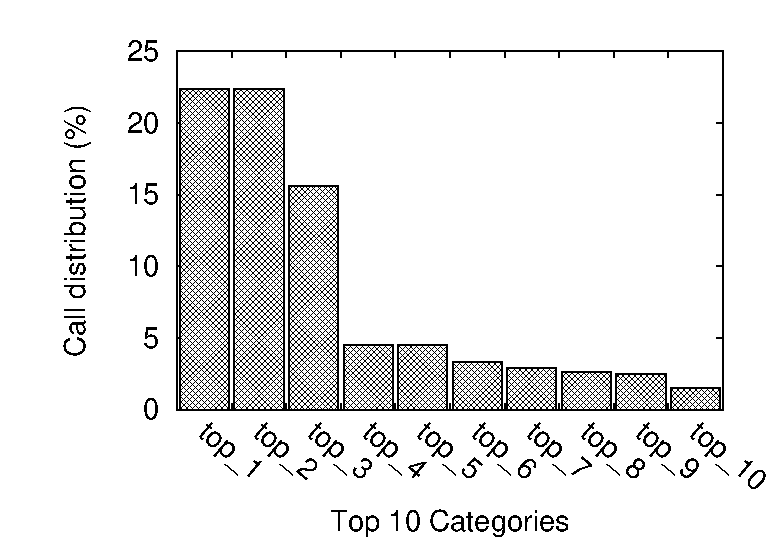
\includegraphics[width=\figurewidthE]{./Figs/category_dist_workgroup.eps}}
\subfigure[Call Resolution (5394 categories)]{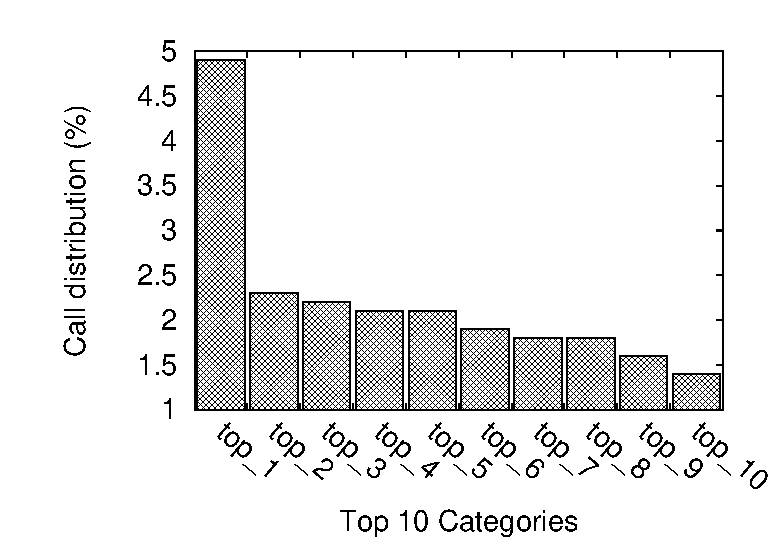
\includegraphics[width=\figurewidthE]{./Figs/category_dist_resolution.eps}}


\subfigure[Level-1 (170 categories)]{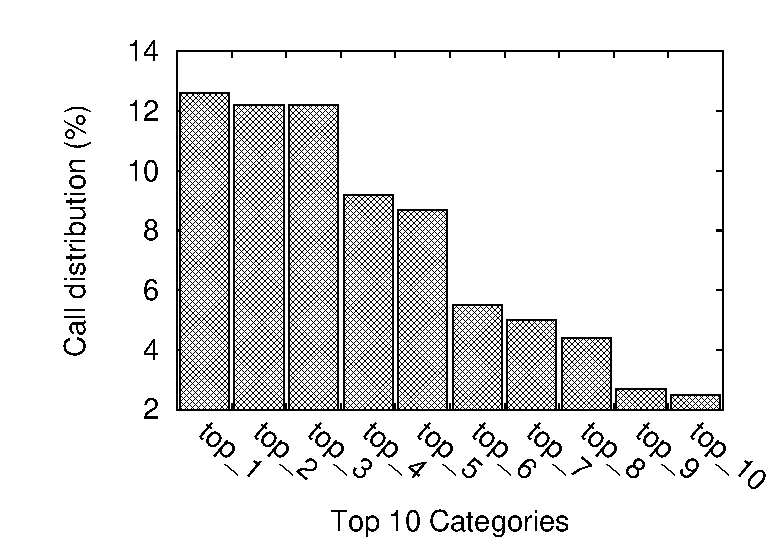
\includegraphics[width=\figurewidthE]{./Figs/category_dist_lv1.eps}}
\subfigure[Level-2 (765 categories)]{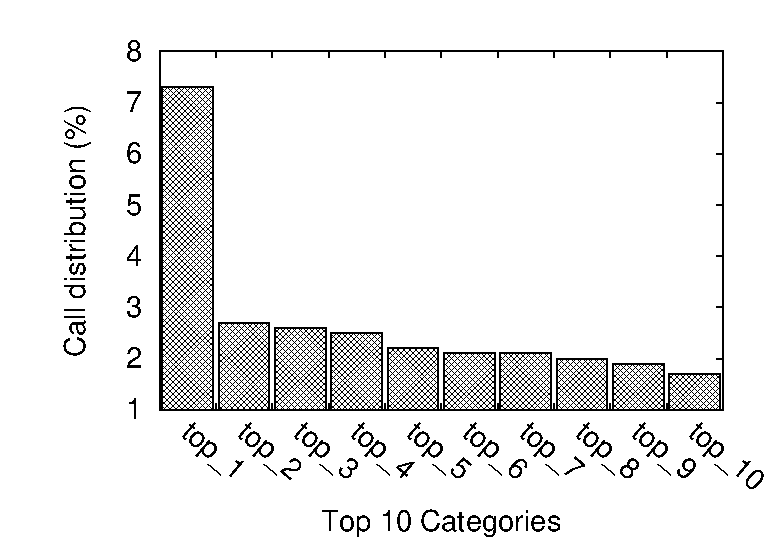
\includegraphics[width=\figurewidthE]{./Figs/category_dist_lv2.eps}}
\subfigure[Level-3 (2882 categories)]{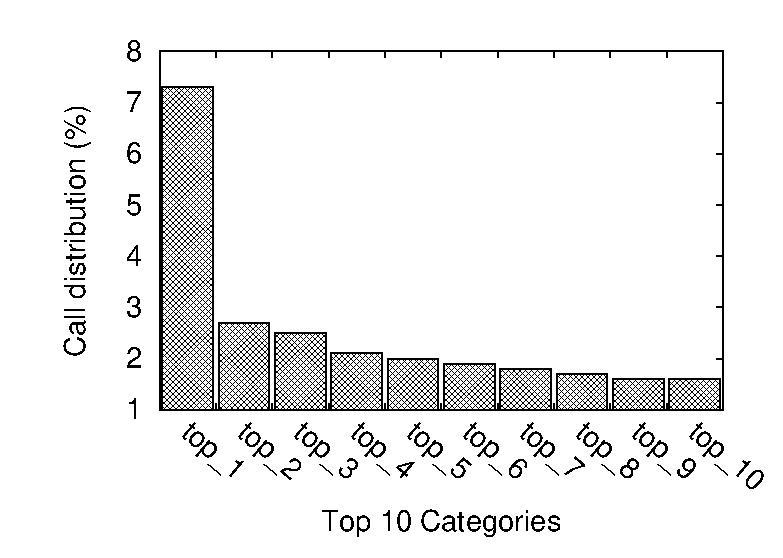
\includegraphics[width=\figurewidthE]{./Figs/category_dist_lv3.eps}}
\caption{The normalized number of calls.}
% \caption{The normalized number of calls in the most popular 10 categories 
% among {\em work group}, {\em call resolution} and 3 levels of {\em customer need}.}
\label{fig:category_distribution}
\end{figure*}


\comment{ %imc-cut
\begin{table}
\centering
\begin{tabular}{|l|c|}
\hline
type of category & \# of predefined classes \\ \hline
work group & 230 \\ \hline
call resolution & 5394 \\ \hline
customer need level 1 & 170 \\ \hline
customer need level 2 & 765 \\ \hline
customer need level 3 & 2882 \\ \hline
\end{tabular}
\caption{Number of predefined classes for each type of category}
\label{tab:categories}
\end{table}
}


\para{Real anomalies:}
In addition, we get ground truth from National Call Center Operations 
(NCCO) reports, in which anomalies are marked manually by monitoring 
the patterns of customer calls, activity of the IVR system, and network traffic. This process is
extremely time-consuming and vulnerable to human errors, which
motivates us to develop an automatic anomaly detector.

Table~\ref{tab:ncco-report} shows an example of NCCO report.
Each anomaly in NCCO reports contains the following information: 
an {\em event status} indicates the anomaly is first reported ({\em initial}),
{\em updated}, or {\em resolved}; a {\em business unit} and {\em primary system} indicate which aspect of system
is impacted by the anomaly; and a {\em region} indicates the impacted region.
A {\em start time} labels the time when the anomaly is observed, and
{\em resolved time} labels the time when the support team reports
that the anomaly has been resolved. In this example, the anomaly is just reported,
so the {\em resolved time} is unknown. There is also a description of the
anomaly, \eg, outage events or performance  degradation. 
We designated the {\em start time} as the time at which an anomaly
is detected. There could be a gap between the time that anomalies are observed 
in NCCO report and perceived by customers.

% XXX: why our method has low recall
Since our approach uses only customer calls data to detect anomalies
while the ground truth from NCCO reports is derived based on the more
complete information (\eg, activity of the IVR system and network traffic), 
we do not expect our approach can detect all anomalies.

\begin{table}
\centering
\begin{tabular}{|l|}
\hline
\textbf{Event Status}: Initial \\
\textbf{Business Unit(s)}: Mobility \\
\textbf{Primary System}: Mobility: GSM Voice Networks    \\     
\textbf{Region}: North East \\
\textbf{Start Time}: month day year - time  \\
\textbf{Resolved Time}: Unknown  \\
\textbf{Issue Description}: Boston customers may experience no service or \\
degraded service in the coverage area of the cell sites affected. \\ 
\hline
\end{tabular}
%\vspace*{-0.15in}
\caption{An example of NCCO report}
\label{tab:ncco-report}
\end{table}

\para{Issues:} The call records give us information about
calls in different categories with different metrics. Each category/metric
gives us one timeseries. Our goal is to automatically detect anomalies or
events using all the timeseries. A natural approach is to detect
sudden changes in one or more timeseries. But finding an appropriate
aggregation of the timeseries for accurate anomaly detection is challenging.

\comment{ %% add another example and rephrase
Simply aggregating all of them does not work well. For example, 
% there are 3 major events: one is {\em iPhone4 new announcement} at June 7
% 2010, one is the {\em start of iPhone4 pre-order} at June 15 2010, and
% the final one is {\em iPhone4 releas} at June 24 2010. 
there were 3 major events related to a release of new devices:
{\em new device announcement},
% on June 7 2010,
{\em new device pre-order},
% on June 15 2010,
and {\em new device available}. 
%on June 24 2010. 
As shown in
Figure \ref{fig:cal-volume-timeseries-day}, 
% if we only
% count the calls that are related to ``iPhone'', we can see clearly
% there are 3 spikes related to the above events during the weeks 6, 7, and 8, respectively.. However, if we ony
% monitor the total call volume, we cannot detect the
% events, because the total volume does not change significantly.
if we consider all the customer care calls that are related to 
a new device, we can see clearly there are 3 spikes in the call volume corresponding 
to the above events. However, the events have little impact on the
total call volume, and are difficult to detect using the total call volume.
}
Simply aggregating all of them does not work well. 
Figure \ref{fig:cal-volume-timeseries-day} show two examples.
In the first example, there were 3 major events related to a release of new devices:
{\em new device announcement},
% on June 7 2010,
{\em new device pre-order},
% on June 15 2010,
and {\em new device available}. 
%on June 24 2010. 
If we consider all the customer care calls that are related to 
a new device, we can see clearly there are 3 spikes in the call volume corresponding 
to the above events. However, the events have little impact on the
total call volume, and are difficult to detect using the total call volume.
In the second example, 3G network outage occurred in South Florida on the second day of the third week.
The anomaly can be detected using the weighted sum of call volume from categories
``Technical'', ``Cannot Make or Receive Calls'', ``Voice'', and
``FLP'' (Florida/Puerto Rico area), but not from 
the total call volume.
% increase of event-related calls is much smaller than the total call
% volume. The other reason is
% Moreover, the capacity limit of call centers places an upperbound on
% the number of serviced calls and limits the change in the total volume
Simply aggregating all calls is insufficient because (i) some events only have
impact on a subset of customers and do not lead to significant changes
in total volume, and (ii) even for the events that may potentially
affect the total volume, the capacity of call centers limits the
increase in total volume and makes it difficult to detect. Ideally in this case, we want to detect
events before the capacity limit is reached so that we can increase
call center capacity temporarily in response to the increased demand.


\begin{figure}
\centering
\subfigure[The three vertical lines indicate the time of 3 major events related to Device-A.]{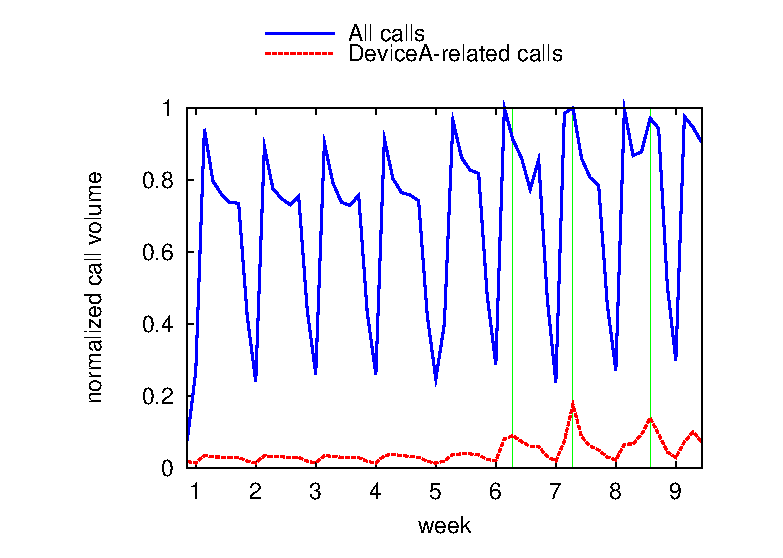
\includegraphics[width=\figurewidthB]{Figs/call_volume_day-norm2.ps}}
\subfigure[An anomaly detected using the weighted sum of several categories]{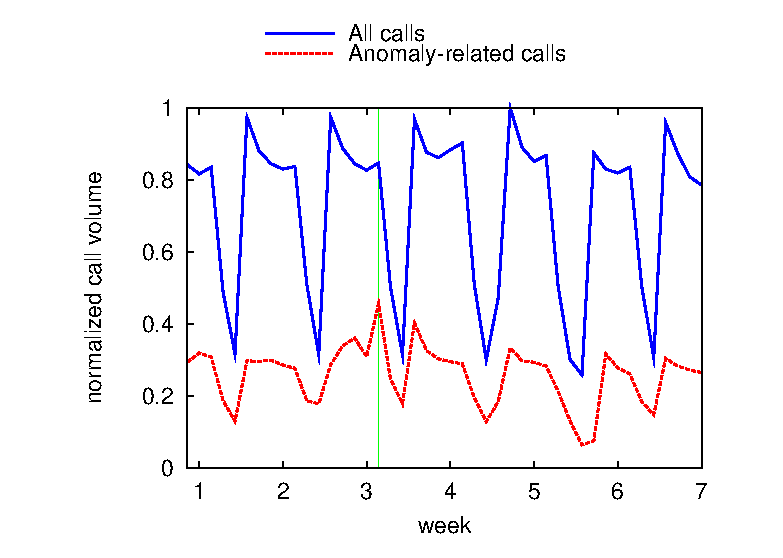
\includegraphics[width=\figurewidthB]{Figs/anomaly_ex_florida.ps}}
\caption{The total call volume is insufficient to detect events.}
\label{fig:cal-volume-timeseries-day}
\end{figure}


% \subsection{Existing approaches}
% \label{ssec:existing-approaches}
% There are several existing anomaly detection schemes. 
% Holt-Winters algorithm (denoted as {\em HW}) builds a seasonal model for call volume time series 
% using past observations and make forecasts. It detects 
% anomalies by comparing the difference and ratio of the predicted value to actual 
% value. 
% Subspace scheme \ref{Lakhina_sig04} decomposes data into normal and abnormal 
% subspaces using PCA. It include 3 steps: (1) Apply PCA to the testing dataset and examine the 
% projection of testing dataset on each principal axis in order. (2) As soon 
% as a projection is found to exceed a threshold (\eg, 2x standard deviation 
% from mean), the principal axis and all subsequent axes are assigned to 
% anomalous subspace. (3) Detect spikes in the time series projected onto the
% anomalous subspace. 

% To show how these existing schemes perform, we compare the precision and recall using
% HW and Subspace schemes with our proposed scheme (denoted as {\em CS}, will explain the detail in Section 
% \ref{sec:approach}) and a random algorithm which report an anomaly with 0.3 probability
% (shown in Figure \ref{fig:existing_schemes}). 
% {\em HW} has low recall which matches what we observe in Section \ref{ssec:case-study} 
% that only monitoring call volume may miss some anomalies. On the other hand,
% {\em PCA} explores the data projection to each principle 
% component and have higher recall. However, because {\em PCA} is known to be 
% sensitive to outliers, the noisy dataset as customer calls can result in low precision as 
% shown in the figure.

Another natural approach to detect anomalies is to use PCA. For example,
\cite{PCA2} decomposes data into normal and abnormal
subspaces using PCA by (i) applying 
PCA to the testing dataset and examining the projection of testing
dataset on each principal axis in order, (ii) assigning the principal 
axis and all subsequent axes to anomalous
subspace as soon as a projection is
found to exceed a threshold (\eg, 2x standard deviation from mean),
and (iii) detecting spikes in the time series projected onto the
anomalous subspace. We observe its precision (\ie, fraction of predicted 
anomalies that are correct) is not much better than that of a random 
algorithm, which reports an anomaly by tossing a bias
coin of 0.3 (\ie, close to the fraction of time that has
anomalies.) 
% XXX: why PCA doesn't work well in detecting anomalies
\comment {
PCA performs poorly because it looks for
orthogonal axes, but orthogonal axes may not represent the most
important metrics. In addition, PCA is sensitive to outliers, which
can be common in noisy customer call dataset.
}
PCA performs poorly for several reasons. First, large anomalies can 
pollute the normal subspace \cite{PCA-sensitivity} so PCA usually requires 
anomaly-free data for training \cite{PCA-unsupervised}. This could be a problem 
for our dataset because there are average 1.8 anomalies per week in NCCO reports 
and it is hard to find a clean period for training. Second, determining the threshold 
for anomalous subspace is an open question \cite{PCA-sensitivity, PCA-structural, PCA2}. 
Third, PCA is sensitive to noise, which is common in the customer care call dataset. 

In general, the appropriate aggregation depends on the types of
events. Due to a large number of possible types of events and
evolving nature of events, it is infeasible to manually determine the
aggregation for each event type in advance. 
The above results call for a new method to automatically learn the
mapping from the various input metrics to anomalies. The method should
be (i) adaptive to new call labels and events, (ii) highly robust
against noise, which is inherent in call data records due to different
customers' responses to anomalies and inconsistent 
call labelings.



%% =================================================================

\section{Our Approach}
\label{sec:approach}

\subsection{Problem Formulation}

Our main problem can be formulated as follow. We have training and
testing traces, where the training traces contain $N$-dimension input
timeseries and the ground-truth about when anomalies take place and
the testing traces contain new $N$-dimension input timeseries. Our
goal is to determine when anomalies occur in the testing traces. 

We use regression to approach
the problem by casting it as an inference problem of $A x = b$, where
$A(t,i)$ denotes the number of calls of category $i$ at time $t$, $x(i)$ denotes
the weight (importance value) of the $i$-th category, $b(t)$ is an
indicator whether there is an anomaly. We construct $A$ and $b$ from the training traces to solve
for $x$. Then we plug in the estimated $x$ and construct $A$ from
the testing traces to predict $b$ for the testing trace. 
Essentially we view there
exists a linear relationship between the categories values and the
resulting anomalies, and we try to learn the linear coefficients $x$
that automatically combines different metrics to predict the
anomalies. 
As we will show in Section~\ref{sec:evaluate}, a 
simple linear regression model works well, so we believe the 
linear assumption is reasonable.
There are several significant challenges involved in realizing this scheme.

\begin{senumerate}
  \item Dynamic $x$: As the categories and events evolve, the
    relationship between the inputs and the anomalies may also
    change. Therefore $x$ can change over time. 
  \item Under-constraints: The number of categories can be much larger
    than the number of constraints derived from the training traces.
    So we have an under-constrained problem and there are an infinite
    number of solutions. Randomly picking one of them gives an equally
    good fit to the training data, but can give very
    different accuracy for the testing data. Our ultimate
    goal is to find $x$ that can accurately predict the
    anomalies for the testing traces.
  \item Over-fitting: Even if we are fortunate to get long enough
    training traces so that the number of categories is close to or
    smaller than the number of constraints, the weight estimation is
    still challenging because the solution that minimizes the fitting
    error based on the training traces is often not the one that gives
    the closest fit to the testing data. In other words, there can be
    over-fitting issues.
  \item Scalability: There are thousands of categories or dimensions
    and thousands of time intervals. The scalability issue further exacerbates
    when we allow $x$ to change. For example, if there are
    $K$ different $x$'s, the problem size further grows by a factor of $K$.
  \item Varying customer response time: When an anomaly
     occurs, customers respond to it at different time depending on
     the impact of anomaly, the customers' own availability, time of
     day, and day of week. This
     blurs the relationship between $A$ and $b$.
     % fuzzy and not well defined. 
\end{senumerate}    

Below we first develop an approach to address the under-constraints
and over-fitting issues while allowing $x$ to change over time
(Section~\ref{ssec:regression}). Then we reduce the number of unknowns
as well as handle the scalability issues by clustering categories and
identifying important clustered categories (Section~\ref{ssec:scalability}). 
Finally, we use multiple classifiers to enhance the
robustness against noise and different customers' response time (Section~\ref{ssec:aggregation}).


\subsection{Our Regression}
\label{ssec:regression}

%As mentioned in Section~\ref{ssec:important}, we can learn the
%importance value of each category by casting the problem as an
%inference problem of $A x = b$. Different from
%Section~\ref{ssec:important}, which aims to pick the important
%metrics, which is a binary decision, accurate predicting future
%anomalies requires us to achieve higher accuracy in the weight
%estimation. More specifically, we formalize the anomaly detection
%problem as follow. Let $A_d(t,i)$ denote the value of $i$-th category
%from the traces at time $t$ on the $d$-th day, $x_d(i)$ denote the
%weight of $i$-th variable on day $d$, $b_d(t)$ denote whether there is
%an anomaly at time $t$ on the $d$-th day, where 1 means anomaly and 0
%means no anomaly.
%
%A natural goal is to also minimize the fitting error to the training
%data. However fitting error alone is insufficient for several reasons. First,
%when the number of categories is smaller than the number of
%constraints derived from the previous traces, we have an
%under-constrained problem and there are an infinite number of
%solutions. Randomly picking one of them gives an equally good
%fit to the previous training data, but can give very different
%accuracy on the testing data in the future. Our ultimate goal is to
%find $x$ such that we can use it to predict the anomalies based on the
%new $A$ derived from the testing traces. Second, if we are fortunate
%to get long enough training traces so that the number of
%categories is close to or smaller than the number of constraints, the
%weight estimation is still challenging because the solution that
%minimizes the fitting error based on the training traces is often not
%the one that gives the closest fit to the testing data. In other words,
%there can be over-fitting issues. 

To address the first challenge, we generalize our formulation to $A_d
x_d = b_d$, where $d$ denotes $d$-th day, $A_d(t,i)$ denote the value
of $i$-th category from the traces at time $t$ on the $d$-th day,
$x_d(i)$ denote the weight of $i$-th variable on the $d$-th day, $b_d(t)$
denote whether there is an anomaly at time $t$ on the $d$-th day,
where 1 means anomaly and 0 means no anomaly.

To address the under-constraints and over-fitting issues, we cannot 
simply minimize the fitting error to the training data. 
Instead, we also impose additional structures on the solution. First, we expect
the weight values $x_d$ to be stable across consecutive days $d$. Second, 
we expect $x = [x_1 x_2 ... x_d]$ exhibits low-rank structure due to
the temporal stability in $x$ and the small number of dominant factors
that cause the anomalies. 
% we expect $x = [x_1 x_2 ... x_d]$ exhibits low-rank structure.
%, because there tends to be a small number of dominant factors. 
Therefore, we 
try to find $X$, $U$, $V$ that minimize the combined objective:
\begin{equation}
o(X,U,V) = \sum_d f(X) + \alpha\cdot g(X) + \beta\cdot h(X,U,V),
\label{eq:c(X)}
\end{equation}
where $f(X)$ is the fitting error, $g(X)$ captures the degree of
temporal stability, and $h(X,U,V)$ captures the error in approximating
$X$ as a product of two rank $r$ matrices: $U$ and $V$, where $\alpha$ 
and $\beta$ give the relative weights of temporal
stability and low-rank constraints, respectively, and $r$ is
the desired low rank.
% Our evaluation uses $\alpha = 0.01$, $\beta = 0.1$, and $r=100$. 
Next we elaborate on each term and how to select weights.

\para{Fitting error:} The fitting error is expressed as
%\begin{align}
$f(X) = \sum_d \left\|A_d x_d - b_d\right\|_F^2$ 
%\end{align}
where $\|\cdot\|_F$ is the Frobenius norm 
% \comment{ %infocom-cut
% ~\cite{wiki:Frobenius-norm} 
% }
(with $\|Z\|_F = \sqrt{\sum_{ij} Z(i,j)^2 }$ for any matrix $Z$.)

\para{Incorporating temporal stability:}
To capture the temporal stability, we introduce
a temporal transformation matrix $T$ and define a penalty
function as follows:
\begin{equation}
g(X) \defas \left\| M \ast T^T\right\|_F^2,
\end{equation}
where $M = [x_1 x_2 ... x_d]$ merges all the column vectors into a
matrix and $T^T$ is the transpose of $T$. As in \cite{zhang09sensing}, we use a simple temporal
transformation matrix to minimize the change in $x$ between two consecutive days:
$T=Toeplitz(0,1,-1)$, which denotes the Toeplitz matrix 
with central diagonal given by 1, the first upper diagonal given by -1. That is, 
{\scriptsize
\begin{equation}
 T = \left[
  \begin{array}{rrrrrrrr}
        1 & -1 &  0 &  \ldots \\
        0 &  1 & -1 &  \ddots \\
        0 &  0 &  1 & -1 & \ddots \\
        \vdots &  \ddots &  \ddots &  \ddots   \\
  \end{array} \right].
\end{equation}
}
\para{Incorporating low-rank constraints:}
Finally, to capture the low-rank nature of weight matrix, we
introduce a penalty term function
\begin{equation}
h(X,U,V) \defas \left\|M - U\ast V^T\right\|_F^2
\end{equation}
where $M = [x_1 x_2 ... x_d]$, $U$ is a $N \times r$ unknown factor matrix, and $V$ is a
$d \times r$ unknown factor matrix, and $r$ is the desired low
rank.  Minimizing the penalty term ensures $M$ has a good rank-$r$
approximation: $M \approx           
U\ast V^T$.

\para{Selecting parameters:}
To decide the weights $\alpha$ and $\beta$, we use 6-week data as the 
training set to find the best weights (in terms of evaluation metrics 
discussed in Section \ref{sec:evaluate}) as follow.
% and use them in our evaluation. 
% The selecting procedure is as following.
First, 
$\alpha$ and $\beta$ are chosen to make fitting error, temporal stability, 
and low-rank constraint have similar order of magnitude. Second, we
fix $\alpha$, and keep increasing or decreasing $\beta$ by a factor of
10 each time until the performance does not improve. 
$\beta$ is updated as the one that gives the best performance seen so far. Third, similar to the second step, 
but this time we fix $\beta$ and alter $\alpha$. The second and third
steps are repeated until the performance does not improve for the
training traces. It usually takes 5 or fewer iterations. 
Then we apply the selected parameters to the testing
trace for anomaly detection. 

%Note that in theory, we do not require a separate step of identifying important
%metrics with the current step of inferring the weights of all metrics
%as one. However, for efficiency purpose, we separate these two steps in our
%approach because the step of identifying important metric requires
%working with all metrics, which are potentially thousands and $L_1$
%norm minimization is light-weight enough to work with thousands of
%metrics.

% \subsection{Data Preparation}
% \label{ssec:preparation}

%% \subsection{Customer Care Call Data} 

%% When a customer calls the customer support,
%% % by dialing the toll free number,
%% the call will first reach an Interactive Voice Response (IVR)
%% system, an automated system configured with
%% pre-defined menu. By selecting through the menu, the customer's call
%% is either self-served
%% % (e.g., checking account balancing)
%% or routed to one of the customer care call centers to be answered by an agent.
%% Work force management for customer call canters are often done
%% according to the type of plan the customer has (\eg, business or
%% consumer) (we refer it as ``work group'' in the paper) and what type
%% of issues the customer has (\eg, device, billing, performance
%% issues). Upon handling each customer care call, the call agent will
%% first open a case in the ticketing system if this is a new issue which
%% has not been reported by the customer before. The call agent will
%% label the case using a three-level pre-defined categories to indicate
%% what issues the customer has or what need the customer asks for (we
%% refer them as ``customer need''). Detailed notes are also input into
%% the system based on the conversation with the customer. After the
%% customer's need is satisfied and case is resolved, a resolution code
%% (we refer it as ``call resolution'') is also tagged into the system
%% according to how the case is resolved.

%% In our study, we use the records that call agents input into their
%% ticketing system. There is a unique record (identified by ticket
%% number) corresponding to each customer care calls that handled by call
%% agents. Each record contains information on timestamps of the start
%% and the end of the customer care call, work group, three levels of
%% customer need, call resolution, and highly coarse grained geographical
%% location of the customer.  Note that the data do not contain
%% information on the customer care calls that are self-served by IVR
%% system or dropped due to long waiting time.

\subsection{Reducing Categories}
\label{ssec:scalability}

The regression problem described in Section~\ref{ssec:regression} has
thousands of variables for each day alone and the number further increases with the
number of days. This imposes both scalability issue and exacerbates
under-constraint issue. 
\comment { % XXX: should we remove it to avoid confusion?
Since top 10\% categories account for 75\%-90\% of calls, one intuitive way to
reduce the number of categories is to use the top 10\% categories. It does not
work for two reasons. First, there are anomalies dominated by categories that are 
not belong to top 10\% categories. For example, the 3G network outage shown in 
Figure~\ref{fig:cal-volume-timeseries-day} is dominated by categories
``Technical'', ``Cannot Make or Receive Calls'', ``Voice'', and ``FLP'' where 
``Technical'' and ``Voice'' are not one of top 10\% categories. 
% 3G network outage is one of the major events that we don't want to miss. 
Second, when new categories are introduced for new services/products, 
the call volume is relatively small at beginning. 
Although the new services/products tend to have more problems, they may be ignored if 
only top 10\% categories are considered. 
Therefore, it's not enough to just focus on these fewer categories.
In this study, we reduce the number of categories using clustering and identifying important
categories. 
}

\subsubsection{Clustering Categories}
\label{ssec:preparation}

% The pre-defined three levels of customer need categories are very fine
% grained.  For example, there are 170, 765, and 2882 unique categories
% in the three levels of customer needs, respectively. As a result,
% there can be multiple categories related to a single type of
% issue. This could cause some ambiguity in the process of hand labeling
% customer care calls by agents. Hence, it is quite common to have
% inconsistency across call agents and call centers.

% To enhance scalability and minimize the
% impact of ambiguity and inconsistency in detecting events based
% on the customer needs categories, we cluster relevant categories based
% on string similarity of their names. In particular, we treat each category name as a sequence of characters and adopt the Dice's coefficient~\cite{wiki:dice} using bigram model~\cite{wiki:bigram}, which is widely used in statistical natural language processing to measure string similarity. 

To enhance scalability and minimize the
impact of ambiguity and inconsistency in detecting events based on the 
customer needs categories, we need to cluster relevant categories in advance.
It is infeasible to group categories manually because (i) the number of categories 
changes over time. Categories can be added or depreciated because of the emerging 
or ending of services/products; (ii) each customer care center can change the usage 
of categories; and (iii) there are too many categories. 

One natural approach is to cluster categories base on  the similarity
between timeseries. However, the approach does not work. 
% Take ``Plan'' and ``Plan and Features'' mentioned in Section~\ref{sec:problem-formulation} as an example. 
For example, Figure~\ref{fig:category_volume_change} shows timeseries of different categories. 
We can see that the call volume of category ``Plans and Features'' increases significantly 
while that of the other category ``Plan'' decreases on the same day, because the agents are 
asked to switch to use ``Plans and Features'' instead of ``Plan''. 
%% give a more complicate example why grouping by timeseries similarity doesn't work:
% XXX: is this a good example? later we actually group categories by name
Similarly, we can see the call volume of ``Device'' decreases while that of ``Account''
and ``Equipment'' increases. Although these categories represent the same group 
of calls, their timeseries are not similar.

% \begin{figure}
% \centering
% 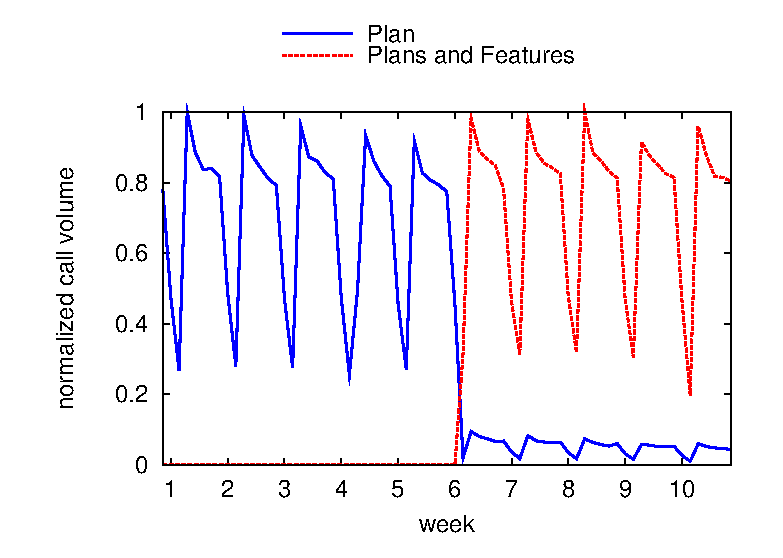
\includegraphics[width=0.4\textwidth]{Figs/top10_ts.ps}
% \vspace{-0.15in}
% \caption{The number of calls labeled as ``Plan'' and ``Plans and Features''. 
% In the second day of the 6th week, call centers use the latter to replace the 
% former.}
% \vspace{-0.15in}
% \label{fig:category_volume_change}
% \end{figure}
\begin{figure}
\centering
\subfigure[The number of calls labeled as ``Plan'' and ``Plans and Features'']{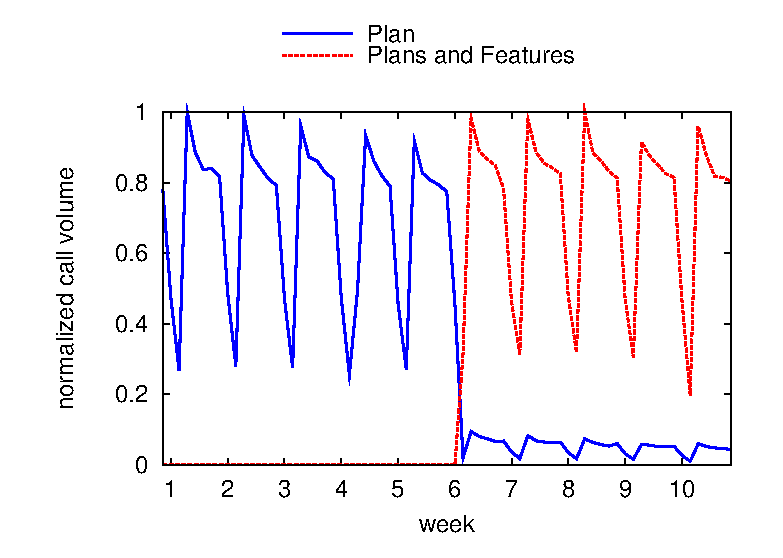
\includegraphics[width=\figurewidthB]{Figs/top10_ts.ps}}
\subfigure[The number of calls labeled as ``Account'', ``Equipment'', and ``Device'' ]{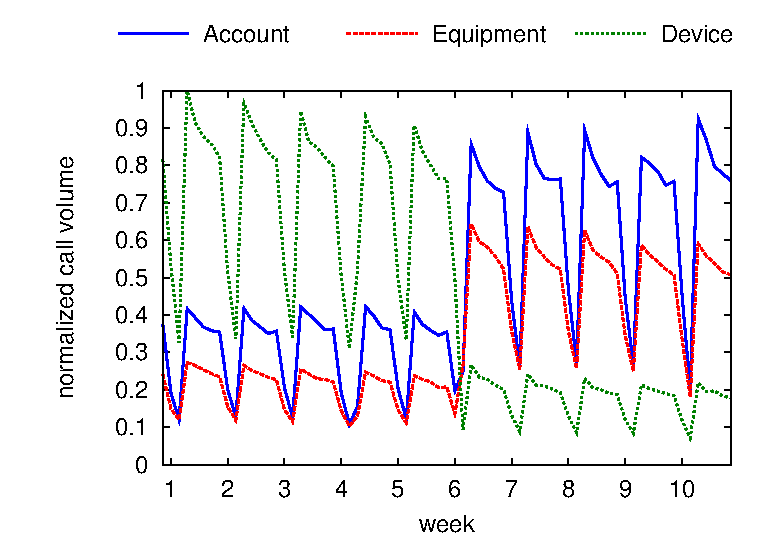
\includegraphics[width=\figurewidthB]{Figs/top10_ts2.ps}}
\caption{Dynamic call labels}
\label{fig:category_volume_change}
\end{figure}

We cluster categories based on the similarity of their textual names
since agents usually classify calls based on the textual names of
categories and different agents may classify similar calls to
different categories with similar texts.
% The clustering method we use is based
% on string similarity of their names.
We treat each category name as a sequence of characters and adopt the Dice's coefficient~\cite{wiki:dice} using bigram model~\cite{wiki:bigram}, which is widely used in statistical natural language processing to measure string similarity. 
The Dice's coefficient $s$ for two string $x$ and $y$ using the bigram model is computed as
$s=\frac{2 \times n_t}{n_x+n_y}$, 
where $n_t$ is the number of character the bigrams in both strings, $n_x$
and $n_y$ are the numbers of big-rams in strings $x$ and $y$,
respectively. The value of $s$ ranges between 0 and 1. A
larger $s$ indicates the two strings are more similar. For example, to
calculate the similarity between strings ``paid'' and ``payment'', we
find the sets of the bigrams as (``pa'', ``ai'', ``id'') and
(``pa'', ``ay'', ``ym'', ``me'', ``en'', ``nt''). These sets have 3 and
6 elements, while only 1 element is common. So we have $s=(2
\times 1)/(3 + 6)=0.22$. By using a threshold of 0.3 for $s$, 
we cluster the customer categories into $96$
at the first level, $354$ at the second level, and $1165$
at the third level. Our evaluate uses these newly computed categories.

\subsubsection{Identifying Important Categories}
\label{ssec:important}

Even after clustering, there are still a large number of clustered
categories. We use the following three schemes to identify important
categories. 

% So we identify important categories by casting this problem
% as an inference problem, and use the following three schemes to solve it.

% We reduce the number of factors by casting the problem
% into an inference problem.In particular, we used and evaluated the 
% following three methods.

\para{Principal component analysis (PCA):} 
% PCA converts a set of
% possibly correlated variables into linearly uncorrelated variables,
% which are called principal components. 
PCA can also be used to identify important categories because
it reduces dimensionality of a multivariate dataset by converting
possibly correlated variables into linearly uncorrelated variables, 
which are called principal components.
% PCA can be performed using
% singular value decomposition of matrix $A$, usually after mean
% centering. 
% XXX: why PCA doesn't work well in identifying important factors
However, using PCA in this context has the same problem as it is used for anomaly detection 
mentioned in Section~\ref{sec:problem-formulation}. As a result,
% The disadvantage of PCA in our context is that 
principal components may not identify the most important categories for 
anomaly detection. For example, 
the 3G network outage event shown in Figure~\ref{fig:cal-volume-timeseries-day}
is dominated by categories ``Technical'', ``Cannot Make or Receive Calls'', ``Voice'', and ``FLP''.
However, the PCA results show that in the top 10\% principal components,
the coefficients of ``Cannot Make or Receive Calls'' and ``Voice'' are small, which
indicates they are not considered as important categories in PCA.


\para{$L_2$ norm minimization:} Another way of finding important
categories is to cast it as an inference problem $A x = b$, where
$A(t,i)$ denotes the value of category $i$ at time $t$, $x(i)$ denotes
the weight (importance value) of the $i$-th category, $b(t)$ is an
indicator whether there is an anomaly. Different from
Section~\ref{ssec:regression}, here we just need to filter out
unimportant categories instead of determining the precise weights. So
here we assume $x$ is constant over time to have fewer unknowns. 

% where $A(t,i)$ denotes the value of category $i$ at time $t$, $x(i)$
% denotes the weight (importance value) of the $i$-th category, $b(t)$
% is an indicator whether there is an anomaly. Essentially we view there
% exists a linear relationship between the categories values and the
% resulting anomalies, and we try to learn the linear coefficients $x$
% that automatically combine different metrics to explain the anomalies.

We obtain $A$ and $b$ learned from
the previous traces. Then we estimate $x$ to best fit the relationship. A
common metric for the best fit is {\em $L_2$ norm minimization},
defined as follows:
%$x$
%which corresponds to (\ref{eqn:reg}) with $J(x) = \|x\|_2^2$.
% $J(\bx) = \|\bx\|_2^2$.
\begin{equation}
% \min_\bx \|{\by} - A {\bx}\|_2^2 + \lambda^2 \|{\bx}\|_2^2.
\min_x \|{b} - A {x}\|_2^2 + \lambda^2 \|{x}\|_2^2,
\label{eqn:L2:0}
\end{equation}
where $\|{x}\|_2 = \sqrt{\sum_{k=1..n} \|x_k\|^2}$.
It can be efficiently
solved using a standard solver for linear least-squares problems.
Then we filter out the categories whose weight $x$ is within a
threshold, which is set to 0 in our evaluation.

\para{$L_1$ norm minimization:} Another approach 
is to use
% (\ref{eqn:y=Ax}) is
{\em $L_1$ norm minimization}, defined as follow: 
% (\ref{eqn:reg}) with 
% $J(\bx) = \|\bx\|_1$ 
%$J(x) = \|x\|_1$ 
% (\ie, the $L_1$ norm of $\bx$).
%(\ie, the $L_1$ norm of $x$).
\begin{equation}
% \min_\bx \|{\by} - A {\bx}\|_2^2 + \lambda^2 \|{\bx}\|_1.
\min_x \|{b} - A {x}\|_2^2 + \lambda^2 \|{x}\|_1.
\label{eqn:L1:0}
\end{equation}
where $\|{x}\|_1 = \sum_{k=1..n} \|x_k\|$. 
$L_1$ norm minimization is often used in situations where 
% $\bx$ 
$x$ 
is
{\em sparse}, \ie, $x$ has only very few large elements and the
other elements are all close to $0$. This is well suited to our goal
of identifying a small number of important factors. As shown
in~\cite{donoho-L1-1}, the minimal $L_1$ norm solution often coincides
with the sparsest solution for under-determined linear systems. As we
will show in Section~\ref{sec:evaluate}, $L_1$ norm minimization performs
the best since it explicitly maximizes sparsity. As before, we filter out the categories whose weight $x$ is within a
threshold, which is set to 0 in our evaluation. 


\subsection{Combining Multiple Classifiers}
\label{ssec:aggregation}

\para{Need for multiple classifiers:} 
Another important problem is what time scale we should use for anomaly
detection. Ideally, we would like to capture all calls triggered
by the same anomaly when learning the weight of the metrics. That is,
$A$ should include the characteristics of all calls corresponding to
that anomaly. However, customers do not respond to an anomaly
immediately and sometimes their response time may differ by hours. But
simply using a large time window is not a good option since we can no longer
detect anomalies in a fine time granularity. 

To address both issues, we use a reasonably small bin size: 1 hour, but include
calls made in previous $n$ and next $m$ hours as additional
features. That is, we use $A_d(t-m,t-(m-1),...,t-1,t,t+1,...,t+n)$, which denotes the values of 
$N$ categories in the traces from time $t-m$ to time $t+n$. 
So there are altogether $(m+n+1) \times N$ features and $x_d$ also now
has $(m+n+1) \times N$ elements, which are the weights of all these
features. $b_d(t)$ remains the same as before (\ie, whether there is
an anomaly at time $t$).

However it is challenging to select $m$ and $n$ a priori. One set of
values may work well on some data but not on others. % The main
% reason is that human respond to anomalies in different ways depending
% on the impact of anomalies, their own availability, and time of
% day.
Therefore we use multiple classifiers, where each classifier uses
one set of $m$ and $n$, and then we aggregate the results of all the
classifiers. The intuition is that it is more likely to be a real
anomaly if lots of classifiers claim so.

\para{Aggregating multiple classifiers:} 
We apply each classifier independently to the testing data and 
returns a binary timeseries $pb(c, t)$. $pb(c, t)=1$ denotes that there 
is an anomaly detected by classifier $c$ at time $t$. $pb(c, t)=0$ 
denotes there is no anomaly detected. We aggregate $pb(c, t)$ by assigning 
a weight $w_c$ to each classifier. We detect an anomaly when $\sum_{c} w_c pb(c, t) 
> threshold$. Our evaluation uses a threshold of 0.3.

We calculate $w_c$ for a classifier $c$ by applying 2-fold 
cross-validation to the training data.
The 2-fold cross-validation partitions the training data into two parts. In 
the first round, it uses the first partition for training and the second partition for 
testing. Since we know the ground truth in all training data, we can evaluate 
how the classifier performs in cross-validation by calculating the accuracy
(\ie, the fraction of correct prediction) in the second partition. Similarly, 
in the second round, we use the second partition of the training data for training, 
use the first partition for testing, and calculate the accuracy in the first partition.
Therefore, with the 2-fold cross-validation we can get an average accuracy $a_c$ in 
training set which gives us an estimate how the classifier may perform.
Then the weight of each classifier is assigned as the normalized 
accuracy: $w_c = a_c / \sum_{c} a_c$.

%% =================================================================


\section{Evaluation}
\label{sec:evaluate}

%\subsection{Evaluation Methodology}

%We evaluate our methods by altering one component at time to see how it impacts 
% the final results.

\begin{figure*}[ht]
    % \centering
    \begin{minipage}{\figurewidthE}%
        \centering
        % 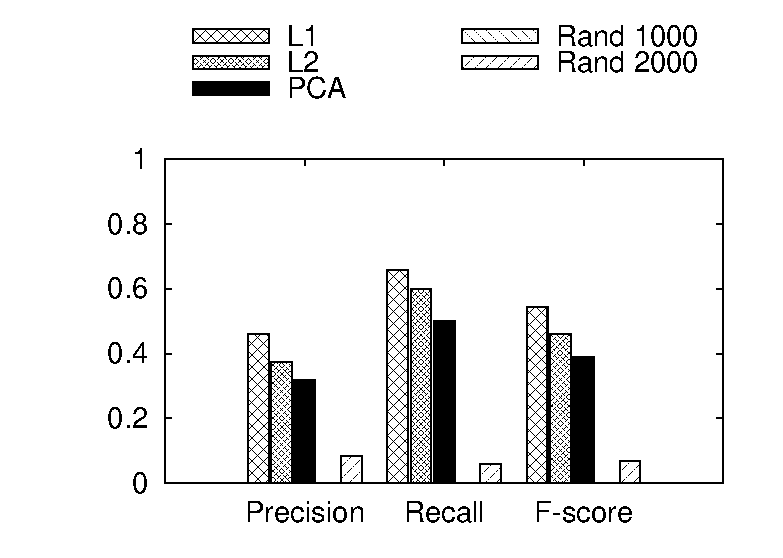
\includegraphics[scale=0.5]{Figs/identify.eps}
        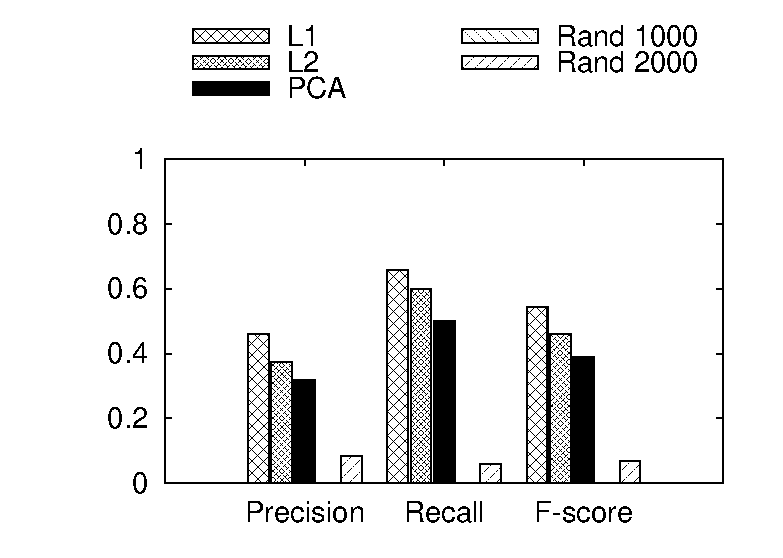
\includegraphics[width=\figurewidthE]{Figs/identify.eps}
        \caption{\small{Varying schemes for features.}}
        \label{fig:identify}
    \end{minipage}
    \begin{minipage}{\figurewidthE}%
        \centering
        % 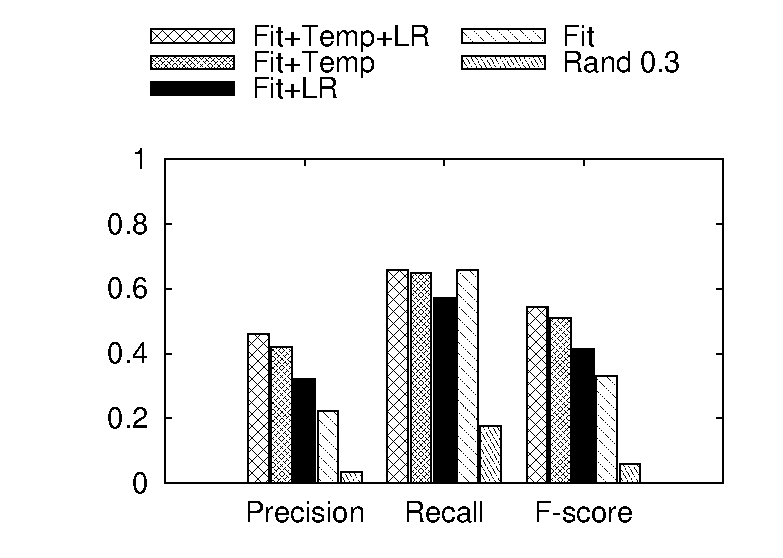
\includegraphics[scale=0.5]{Figs/regression.eps}
        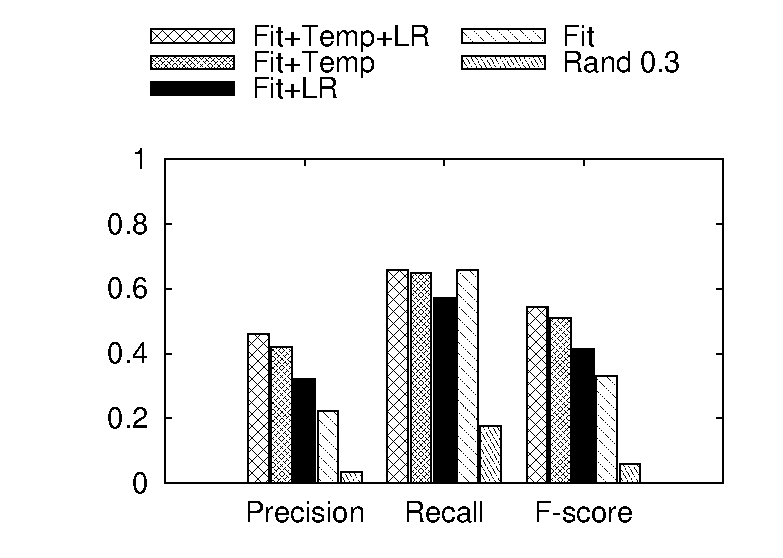
\includegraphics[width=\figurewidthE]{Figs/regression.eps}
        \caption{Varying regression methods.}
        \label{fig:regression}
    \end{minipage}
    \begin{minipage}{\figurewidthE}%
        \centering
        % 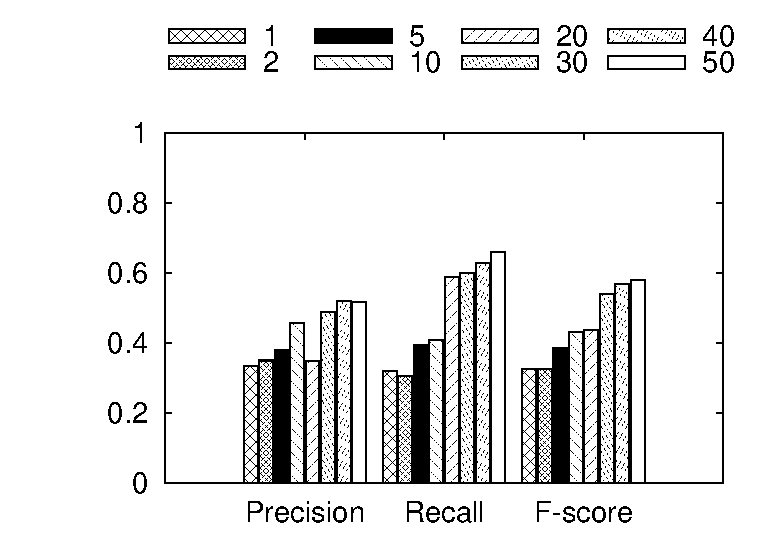
\includegraphics[scale=0.5]{Figs/multi-num-classifier.eps}
        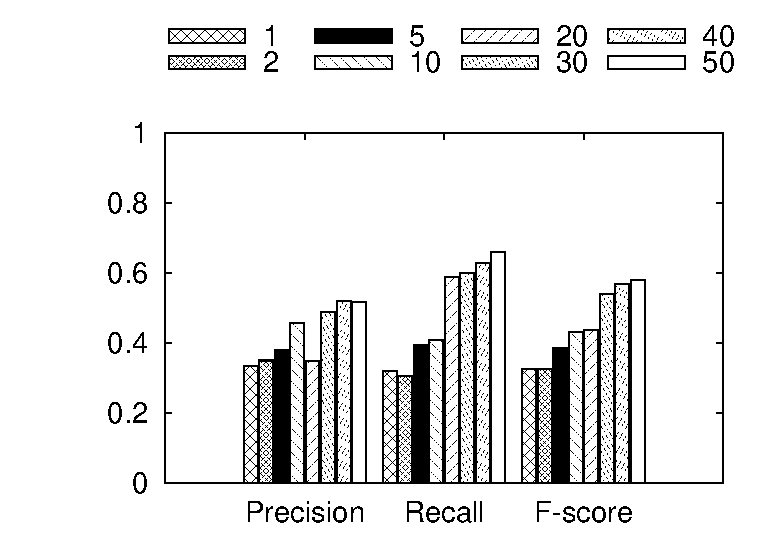
\includegraphics[width=\figurewidthE]{Figs/multi-num-classifier.eps}
        \caption{Varying the number of classifiers.}
        \label{fig:multi-num-classifier}
    \end{minipage}
\end{figure*}


We use the following metrics to quantify the accuracy:
\begin{align}
&recall = \frac{tp}{tp+fn}\\
&precision = \frac{tp}{tp+fp}
\label{eqn:metric}
\end{align}
% \begin{equation}
% accuracy = \frac{tp+tn}{tp+tn+fp+fn}
% \label{eqn:accuracy}
% \end{equation}
where $tp$ is the number of true positives (\ie, correctly detected anomalies),
$fp$ is the number of false positives (\ie, incorrectly detected anomalies),
% $tn$ which denotes $true negative$ are the correct obsense of anomalies, 
and $fn$ is the number of false negatives (\ie, missed anomalies).
In addition, we integrate precision and recall into a single metric
called {\em F-score}~\cite{wiki:F-score}, which is the harmonic mean
of precision and recall: {\em F-score} $ = \frac{2}{1/precision +               
1/recall}$. For all three metrics, larger values indicate higher accuracy.
Unless otherwise specified, we use 30 classifiers.

%\subsection{Performance Results}

% use the best regression and try L1, L2, random, textual based
% etc. to show L1 is the best

\para{Identification of important features:} We first evaluate how 
different feature selection algorithms impact 
the performance. We vary the methods of identifying important
categories while using multiple
classifiers and temporal/low-rank based regression. We compare PCA, $L_1$ norm minimization, $L_2$ norm
minimization, and random selection (\eg, {\em Rand 1000} and {\em Rand
 2000} randomly select 1000 and 2000 categories). $L_1$ norm selects 612 important categories and $L_2$ norm selects 980 important categories.
As shown in Figure \ref{fig:identify}, $L_1$ norm consistently
performs the best. It out-performs $L_2$ norm by 23\%, PCA by 45\%,
Rand 2000 by 454\% in terms of precision; out-performs $L_2$ norm by
10\%, PCA by 32\%, and {\em Rand 2000} by 1020\% in terms of
recall. {\em Rand 1000} selects too few categories and yields close to
0 precision and recall, so its bars are almost invisible from the figure.

%% {\em L1} denotes $L_1$ norm minimization which selects 212 categories
%% from our data set, and {\em L2} denotes $L_2$ norm minimization which
%% selects 802 categories.  {\em PCA} transforms the customer call data
%% to a new coordinate system such that the greatest variance by any
%% projection of the data comes to lie on the first coordinate and we
%% select the first $n$ coordinates that accounts for 99\% of the
%% variance, which is typically 200-250.  {\em Rand 1000} and {\em Rand
%%   2000} are the baseline algorithms which randomly select 1000 and
%% 2000 categories. The results show that {\em Rand 1000} has low
%% probability to select important categories and both precision and
%% recall are 0. {\em Rand 2000} also performs much worse than {\em L1}
%% and {\em L2}. The precision of {\em L1} is 23\% better than that of
%% {\em L2}, 45\% better than {\em PCA}, and 454\% better than {\em Rand
%%   2000}.  The recall of {\em L1} is 10\% better than that of {\em L2},
%% 32\% better than {\em PCA}, and 1020\% better than {\em Rand 2000}.



\comment{ % combine to one row
\begin{figure}
\centering
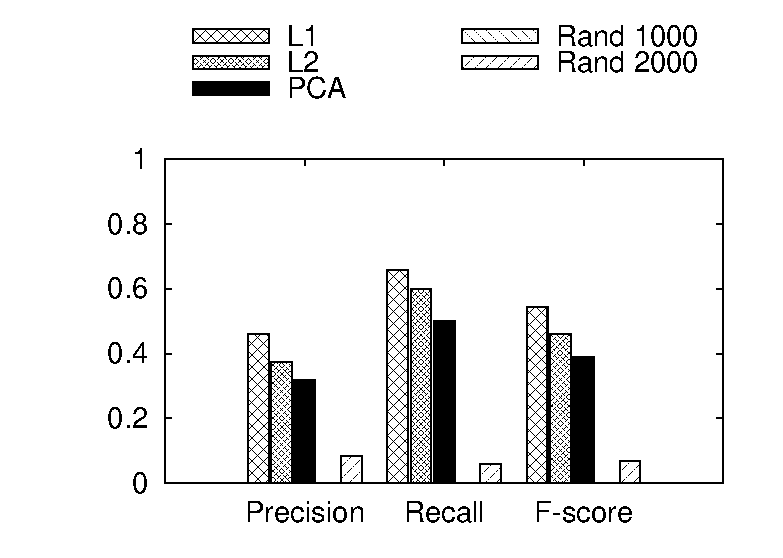
\includegraphics[\figurewidthA]{Figs/identify.eps}
\caption{Identify important features}
\label{fig:identify}
\end{figure}
}

% use L1 to select features and try 1) compressive sensing based regression, 
% 2) pure regression, 3) low rank + regression, 4) temporal stability + regression,
% 5) random
\para{Varying regression methods:} Next we evaluate the impact of
regression methods. We use $L_1$ norm minimization to select important
categories and use multiple classifiers in all cases. We compare
regression (i) that only uses fitting error as the objective ({\em Fit}),
(ii) that uses fitting error and low rank ({\em Fit+LR}),
(iii) that uses fitting error and temporal stability
({\em Fit+Temp}),
(iv) that uses fitting error, temporal stability, and low rank
({\em Fit+Temp+LR}). In addition, as a baseline, we use random
selection (Rand 0.3) that randomly determines if a given interval has an anomaly with a
probability of 0.3 since around 30\% of time intervals have anomalies. 
As shown in Figure~\ref{fig:regression}, Fit+Temp+LR
yields the highest accuracy: it out-performs Random, Fit, Fit+LR,
Fit+Temp by 823\%, 64\%, 32\%, 6\%, respectively, in terms of
F-score.

% fitting error based regression (Fit), fitting error and low-rank based
% regression (Fit+LR), fitting error and temporal stability based
% regression (Fit+Temp), and fitting error, temporal stability and low
% rank (Fit+Temp+LR)

%{\em CS} shows the results of compressive based regression.  {\em T}
%is the scheme that incorporates fitting error with only temporal
%stability (\ie, set $\alpha$ to 0 in Eq. \ref{eq:c(X)}.) In {\em LR},
%we incorporate only low-rank constraints (\ie, set $\beta$ to 0 in
%Eq. \ref{eq:c(X)}.)  In {\em R}, we minimize only fitting error by
%setting $\alpha$ and $\beta$ to 0 in Eq. \ref{eq:c(X)}. {\em Rand
%  0.5}, {\em Rand 0.3}, and {\em Rand 0.1} are schemes that randomly
%determine if there is an anomaly each time with independent
%probability 0.5, 0.3, and 0.1 respectively. The results for precision
%show that compressive sensing based regression outperforms all {\em
%  T}, {\em LR}, {\em R}, {\em Rand 0.5}, {\em Rand 0.3}, and {\em Rand
%  0.1} schemes by 10\%, 43\%, 109\%, 423\%, 1308\%, 869\%
%respectively.  Because {\em Rand 0.5} mark 50\% of time as anomalous,
%there is high probability that real anomalies are also marked as
%anomalous. This leads {\em Rand 0.5} a high recall but very low
%precision. Otherwise, compressive sensing based regression performs
%best in recall.

\comment{ % combine to one row
\begin{figure}
\centering
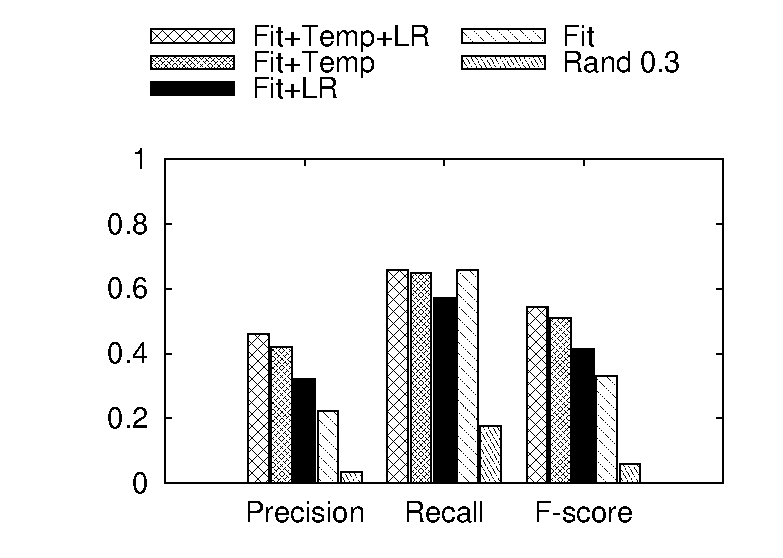
\includegraphics[width=\figurewidthA]{Figs/regression.eps}
\caption{Varying regression methods.}
\label{fig:regression}
\end{figure}
}

\para{Using multiple classifiers:} We evaluate how the number of
classifiers affects the performance. As shown in
Fig. \ref{fig:multi-num-classifier}, leveraging more classifiers can generally
improves the accuracy, as we would expect. The improvement increases
significantly initially and then tapers off. Since the computation
cost increases with the number of classifiers, we use 30 classifiers as the default 
to trade off the benefit and cost.
% prefer to use fewer classifiers.
% that yields good performance. So we use 30 classifiers as the default. 

%give us better results. It is because a single classifier apply one
%set of parameters in our system and which may not work well in all
%cases. For example, for some training set, there are only a few
%anomalies and may need to put higher weight on these anomalies.
%However, the same weight could lead a bias in training set which has
%more anomalies.  By setting combining more classifiers we can have a
%stronger classifier which accommodate the variance in the dataset.
%
%On the other hand, more classifiers also mean the approach takes more
%time to run.  Our goal is to provide a real-time anomaly detection
%tool, so we don't want to include all classifiers. From
%Fig. \ref{fig:multi-num-classifier}, we choose to use 30 classifiers
%which has similar performance as that with 50 classifiers.  

% \begin{figure}
% \centering
% \includegraphics[width=\figurewidthA]{Figs/multi-identify.ps}
% \vspace{-0.15in}
% \caption{Varying the schemes to identify important features (using
%   multiple classifiers).}
% \vspace{-0.15in}
% \label{fig:multi-identify}
% \end{figure}

% \begin{figure}
% \centering
% \includegraphics[width=\figurewidthA]{Figs/multi-regression.ps}
% \vspace{-0.15in}
% \caption{Varying regression methods for anomaly detection (using
%   multiple classifiers).}
% \vspace{-0.15in}
% \label{fig:multi-regression}
% \end{figure}

\comment{ % combine to one row
\begin{figure}
\centering
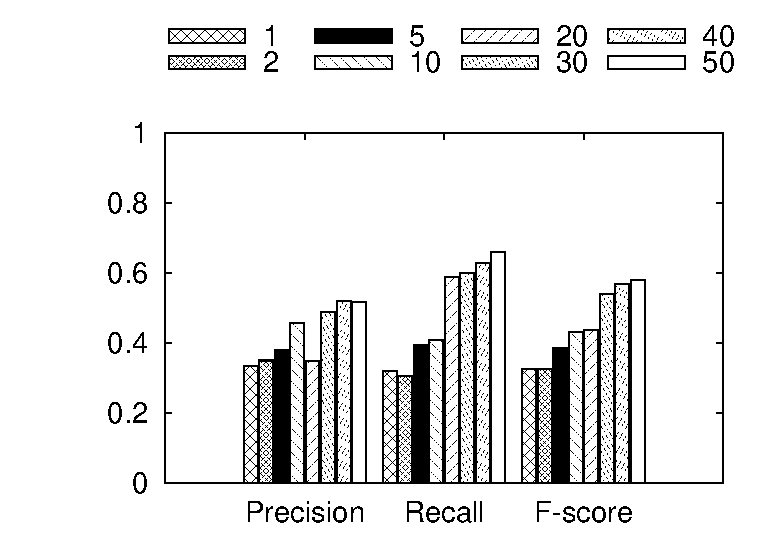
\includegraphics[width=\figurewidthA]{Figs/multi-num-classifier.eps}
\caption{Varying the number of classifiers.}
\label{fig:multi-num-classifier}
\end{figure}
}

\para{Varying the sizes of training sets:} We use the previous $n$ 
days as the training set and detect anomalies on the next day. As
shown in Figure
\ref{fig:multi-train-test}, when $n$ increases from 7 days to 42 days, 
the recall increases from 46\% 
to 79\%, but when $n$ increases from 42 days to 63 days, the recall drops 
to 51\%. Similarly, when $n$ increases from 7 days to 21 days, the 
precision increases from 44\% to 61\%, but a further increase in $n$ to 
63-day reduces the precision to 32\%. It is because when training set is larger, 
we have more constraints to find a better solution for Eq. \ref{eq:c(X)} and
therefore a higher accuracy. However, as the training set further
increases and includes older dataset, the performance may degrade due to the
evolving nature of the dataset. We plan to place higher weights to the
constraints learned from more recent dataset to further improve the
accuracy and robustness in the future.
% weights to the constraints derived from different time to 

% because our dataset is noisy, the performance may degrade with 
% could be impaired by the noise introduced. 

\begin{figure}
\centering
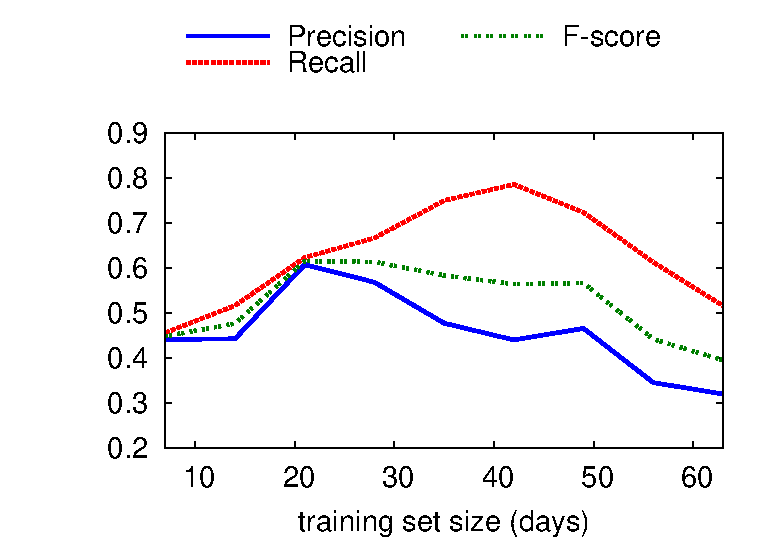
\includegraphics[width=\figurewidthA]{Figs/multi-train-test.ps}
\caption{Varying the size of training set.}
\label{fig:multi-train-test}
\end{figure}


\para{Varying ratios of weight:} Let $x(i, t)$ denote the 
weight (importance value) of the $i$-th category at time $t$. The change 
ratio of weight is $\sum_{t} \sum_{i} (x(i, t) - x(i, t-1))/x(i, t-1)$ when 
$x(i, t-1)$ is not $0$. % Figure~\ref{fig:x_diff_ratio} shows the CDF of 
% the change ratio. From the figure, 
We see 84\% of the changes is
within 10\%, and 2.5\% of the changes is larger than 100\%. This
suggests $x$ has significant temporal stability, but it can also
adapt to different values in order to detect different types of
anomalies across two consecutive days.

% occasionally due to different types of anomalies
% which means that most of time the weight changes littdoesn't change
% much. However, there are 15\% of change ratio is larger than 100\%
% which means there exists dynamic from day to day. It may because two
% continuous days have different type of anomalies which requires
% different set of weight to detect them.

\comment{ %imc-cut
\begin{figure}
\centering
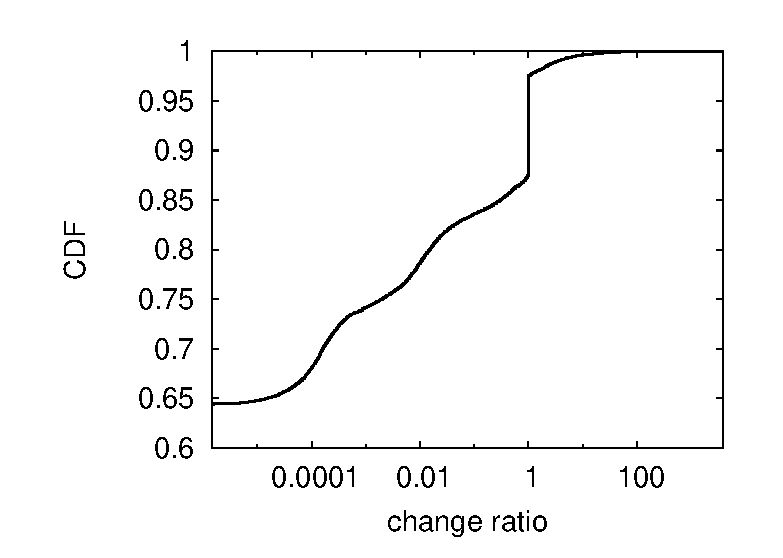
\includegraphics[width=\figurewidthE]{Figs/xdiff.eps}
\caption{CDF of the amount of change between intervals.}
\label{fig:x_diff_ratio}
\end{figure}
}



%% =================================================================


\section{External Data: Social Media}
%\section{External Data Sources}
\label{sec:twitter}

So far, we focus on event detection using the call records,
which are the direct feedbacks from customers.
However, it is hard to understand the nature of detected events from customer calls
due to the following reasons:
(i) Categories from call records only have limited text
information to describe the issues behind the calls.
(ii) Locations of the called customers can be inferred by the area codes of their phone numbers.
However, the coverage of each area code is not uniform.
Moreover, the customers may use the area codes from their previous locations.
% market regions,
%which coverages are not uniform. Some coarse grained markets (\eg, Florida/Puerto-Rico) 
%consist of multiple states, where others (\eg, Rio Grande Valley, TX) are in finer granularity.
%There are other potential data sources that we can take
%advantage of. 

\para{Benefits of using Twitter:}
To better understand the detected events, we leverage Twitter social media
as an indirect channel to understand customers' experience of the service.
There are mainly three reasons that make Twitter social media an attractive data source.
First, Twitter data is massive; as of March 2012, Twitter has 500 million registered users~\cite{massive-twitter}.
%people have embraced social media as the channel to express themselves
Many people share their experiences of the services and products they are using.
Second, user feedbacks are coming in near real-time. Compared with the efforts to report 
issues through customer calls, it is much easier to express their experiences through \emph{tweets}. 
Third, tweets may have richer context information than customer calls. They have many features which help to
understand the various events.

%Here we report our initial experience of using Twitter social media data with customer call records.
% Twitter is another source where we can get user feedback economically.
% In this section, we shows a preliminary results of exploring 
% the correlation between Twitter data and customer calls. 

\para{Data description:}
Twitter data comes with a variety of features, which will help us to 
understand the nature of detected events. 
We use the following features of tweets:
% Below we describe the features used for the analysis:
\begin{itemize}
\item Timestamp; 
\item Text of original tweets
\item Text of normalized tweets, which are the tweets converted into a standard format to ease processing; 
\item Username: a tweet's author;
\item Twitter specific features: URLs, retweets (RT), \#hashtags used to mark keywords or
  topics in a tweet, and @mentions, which are the tweets containing ``@username'' anywhere in the text;
% We find that \#hashtags are useful to extract our interested tweets;
\item Location (city, state, latitude, longitude): Locations can come from the 
tweets themselves or Foursquare~\cite{foursquare/API}. %(will describe the details below). 
%In other cases, we join the location
%information from Foursquare~\cite{foursquare/API} by matching the Twitter username. 
\comment{ %infocom-cut
\item Sentiment: we use the sentiment analysis algorithm from \cite{sentiment} 
to measure the subjectivity (\eg, if the content is objective or subjective)
and the polarity (\eg, if the tweet contains positive or negative messages).
}
\comment{ %infocom-camera-ready-cut
\item Problem detection: we apply the problem detection method from \cite{problemdetect} to find the problematic tweets (\eg, indicating a problematic situation such as outages, call drops, etc.)
}
% classify the tweets
% into two categories: problematic tweets (\eg, indicating a problematic situation such as outages, call drops, etc.) and non-problematic tweets.
\end{itemize}


\begin{table*}
  {\small
\begin{center}
  \begin{tabular}{ | p{5cm} || l | p{7cm} |  }
    \hline
        Event & Location & Event summary by TF-IDF\\ \hline
    \hline
        % %2011-06-28 & 21:00 - 23:00 & Miami, FL & 3g, service, florida, outage, south, network, miami, turn \\ \hline
        3G network outage & New York, NY & service, outage, nyc, calls, ny, morning, service \\ \hline
        outage due to an earthquake & East Coast & \#earthquake, working, wireless, service, nyc, apparently, new, york \\ \hline
        3G network outage & Miami, FL & outage, south, service, issue, broward (a county in FL), key, west, equipment, Florida \\ \hline
        Internet service outage & Bay Area & serviceU, bay, outage, service, Internet, area, support, \#fail \\ \hline
        New device release & Nationwide & iphone, sprint, verizon, apple, 4s, android, accessibility \\ \hline
        New device release & Nationwide & 4s, apple, iphone, \#iphone4s, pre-order, order, site, \#apple, store \\ \hline
  \end{tabular}
\end{center}
\caption{
Examples of detected anomalies with the summary. 
% They are confirmed by the NCCO reports (the date and time of events are not shown due to proprietary issue.)
}
%\vspace*{-0.15in}
\label{table:att-events}
}
\end{table*}

\para{Understanding detected events:} Once the anomalies are detected,
we can leverage various features of tweets, such as keywords and locations, to summarize events as follow. We first find tweets that are related to customers experience
by selecting tweets with hashtag \#XXXFAIL or \#XXXSUCK during the
entire period, where XXX denotes the name of the provider. Then we try to identify important keywords that appear in the anomaly period. We use the metric, called Term Frequency - Inverse Document Frequency (TF-IDF)~\cite{TFIDF}, to quantify the importance of a keyword. TF-IDF is defined as the number of occurrences of word-level 1-grams and 2-grams during the period of the anomaly (in the selected tweets) divided by the number of occurrences in the entire period (in the selected tweets). The intuition is that a keyword that appears frequently only in the anomaly period but not universally frequently is important. Table~\ref{table:att-events} shows some examples of events summarized using this approach. 

% these tweets and is not used as a search key (\eg, \#XXXFAIL or \#XXXSUCK) is important, since the search keys already appear in all these selected tweets. Table~\ref{table:att-events} shows some examples of events summarized using this approach. 

% Given the start and end time of an anomaly, we summarize the anomaly
% by extracting keywords from tweets within that time frame using Term
% Frequency - Inverse Document Frequency (TF-IDF)~\cite{TFIDF}.  We
% first identify tweets that are related to customers experience by
% selecting tweets with hashtag \#XXXFAIL or \#XXXSUCK, where XXX
% denotes the name of the provider. Second, we define Term Frequency as
% the frequency of word-level 1-grams and 2-grams in the selected tweets
% during the time frame of the anomaly. Third, Inverse Document
% Frequency is defined by dividing the total number of word-level
% 1-grams and 2-grams in the collected tweets by the number of
% word-level 1-grams and 2-grams in the second step.  Finally, for each
% word-level 1-gram and 2-gram in the collected tweets during the time
% frame of the anomaly, we calculate the product of its Term Frequency
% and Inverse Document Frequency to see how important this n-gram is in
% the time frame of the anomaly.  Table~\ref{table:att-events} shows
% some examples of using this approach to describe anomalies.

% we use Term Frequency - Inverse Document Frequency (TF-IDF)~\cite{TFIDF}, which is a popular method to 
% identify representative keywords from 
% documents. TF counts the keyword occurrences in the target tweets, whereas IDF looks at
% the popularity of the keywords in the universe documents. For example, a keyword used for filtering will  
% have a low TF-IDF score because it will appear in most of the tweets
% in the dataset, while outstanding keywords will have higher TF-IDF scores.

\begin{figure}
\centering
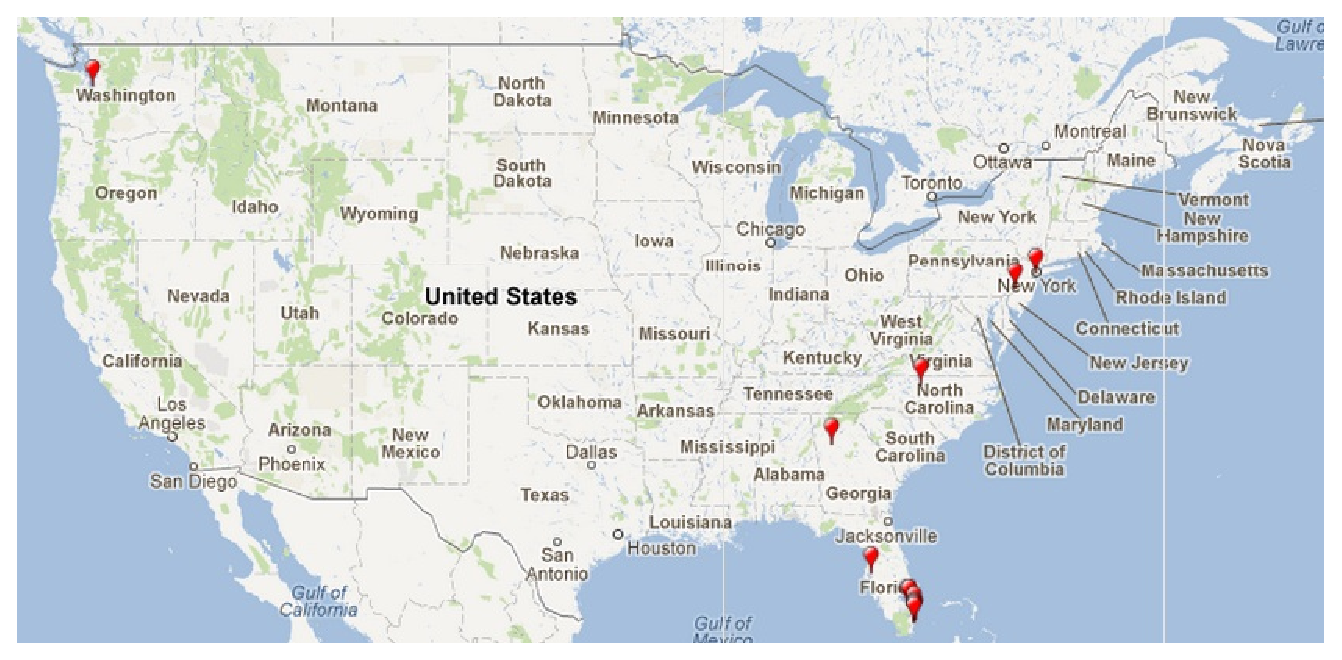
\includegraphics[width=0.6\columnwidth]{Figs/miami.eps}
\caption{
Tweet locations of an detected event.}
\label{fig:miami}
\end{figure}

To locate the impacted regions of the given anomaly,
we gather the authors of the collected tweets, which contains n-grams with high TF-IDF scores 
during the time frame.
Then we check the locations of the authors to get the impacted regions.
Figure~\ref{fig:miami} shows an example of the tweet locations for the anomaly occurred at Miami, 
FL. Although some users may tweet about network incidents from other locations,
as long as we see multiple tweets in a region, we can correctly locate the anomaly.  


%% =================================================================
\section{Conclusion}
\label{sec:conclusion}

We develop a systematic method to automatically detect anomalies in a
cellular network using the customer care call data. Our approach scales to a
large number of features in the data and is robust to 
noise. Using evaluation based on the call records collected from a
large cellular provider in US, we show that our method can
achieve 68\% recall and 86\% accuracy, much better than the existing
schemes.
Moreover, we show that social media can be used as a complementary source
to get higher confidence on the detected anomalies and to
summarize the user feedbacks to anomalies with text and location information.

%% =================================================================

\chapter{Robust Compressive Sensing}
\index{Robust Compressive Sensing@\emph{Robust Compressive Sensing}}
\label{chp:robust-cs}

In this chapter, we develop LENS decomposition, a novel technique to accurately decompose network data represented in the form of a matrix into a low-rank matrix, a sparse anomaly matrix, an error term, and a small noise matrix. This decomposition naturally reflects the inherent structures of real-world data and is more general than existing compressive sensing techniques by removing the low-rank assumption and explicitly supporting anomalies.


\section{Analysis of Network Matrices}
\label{sec:measurement}

\begin{table}[htb]
  \centering
  {\small
    \vspace{-0.1in}
  \begin{tabular}{|@{~}l@{~~}|@{~~}l@{~}|@{~~}l@{~}|@{~~}l@{~}|@{~~}l@{~}|}
\hline
Network & Date & Duration & Resolution & Size  \\\hline
3G traffic & Nov. 2010 & 1 day & 10 min. & $472 \times 144$ \\\hline
WiFi traffic & Jan. 2013 & 1 day & 10 min. & $50 \times 118$ \\\hline
Abilene traffic~\cite{abilene} & Apr. 2003 & 1 week & 10 min. & $121 \times 1008$ \\\hline
G\'{E}ANT traffic~\cite{uhlig06:_provid} &  Apr. 2005 & 1 week  & 15 min. & $529 \times 672$ \\\hline
1 channel CSI & Feb. 2009 & 15 min. & 1 frame & $90 \times 9000$ \\\hline
multi. channels CSI & Feb. 2014 & 15 min. & 1 frame & $270 \times 5000$\\\hline  % 30 subcarriers * 9 channels
% Sensor & Feb. 2004 & 1 day & 10 min. & $54 \times 144$ \\\hline
Cister RSSI~\cite{RSSI1} & Nov. 2010 & 4 hours & 1 frame & $16 \times 10000$ \\\hline
CU RSSI~\cite{RSSI2} & Aug. 2007 & 500 frames & 1 frame & $895 \times 500$ \\\hline
UMich RSS~\cite{UMich-RSS} & April 2006 & 30 min. & 1 frame & $182 \times 3127$
\\\hline     % 14 * 13 pairs
UCSB Meshnet~\cite{UCSB-Meshnet} & April. 2006 & 3 days & 1 min. & $425 \times 1527$ \\\hline  % 38 * 38 pairs
%RON delay~\cite{RON} & Mar. 2001 & 2 days & 5 min. & $144 \times 494$ \\\hline
  \end{tabular}
  }
  \caption{Datasets under study.}
  \label{tab:data}
\end{table}

\subsection{Datasets}
\label{ssec:data}

Table~\ref{tab:data} lists the network matrices used for our
study. 
We obtained 3G traces from 472 base stations in a downtown area of a major city
% with a population of 8.7 million people,
in China during Oct. 2010. 
We generate traffic matrices by computing the aggregated traffic every 10
minutes. $M(i,t)$ represents the total traffic volume to and from base station
$i$ during time interval $t$, where $t$ is a 10-minute interval.
% A row in the traffic matrix represents the traffic time-series a base
% station while a column represents the aggregated traffic of base
% stations in the 10 minutes bin.

We also got WiFi traffic from a large university in China, and
generated traffic matrices based on the traffic collected at the 50 most
loaded access points (APs) on Jan. 4, 2013. $M(i, t)$ denotes
the total traffic to/from AP $i$ during the $t$-th 10-minute
time interval. 

In addition to wireless traffic matrices, we also
use traffic matrices from Abilene (Internet2)~\cite{abilene}
and G\'{E}ANT~\cite{uhlig06:_provid}, which are standard traffic matrices
used in several previous studies (\eg,
\cite{PCA2,lakhina04:_pca,anomography,zhang09sensing}) and useful for
comparison. Abilene traces report total end-to-end traffic between all pairs
in a 11-node network every 10 minutes. G\'{E}ANT traces report total traffic
between all pairs in a 23-node network every 15 minutes. 

For diversity, in addition to traffic matrices, we also obtain signal
strength and expected transmission time (ETT). % and Internet delay traces
We use the following SNR and RSS
matrices: (a) our 1 channel CSI traces, (b) our multi-channel CSI traces, (c) Cister RSSI traces, (d) CU
RSSI traces, and (e) UMich RSS. We collected (a) 
by having a moving desktop transmit back-to-back to another desktop and letting the receiving
desktop record the SNR across all OFDM subcarriers over 15 minutes
% sensor traces, and human traffic matrices in a social network.
% We get CSI traces by
% having two desktops as the sender and the receiver.
% Each desktop is
% equipped with
using the Intel Wi-Fi Link 5300 (iwl5300) adapter. The
modified driver~\cite{iwlagn} reports the channel matrices for 30
subcarrier groups in a 20MHz channel, which is about one group for every two subcarriers according to the standard~\cite{802.11n-2009}. The
sender sends 1000-byte frames using MCS 0 at a transmission power of
15 dBm. Since MCS0 has 1 stream and the receiver has 3 antennas, the
NIC reports CSI as a $90 \times 1$ matrix for each frame. 
% We walked
% with the sender and had the receiver record the CSI of the received
% frames for 15 minutes.
% The CSI matrix $M(t,f)$ denotes the SNR in the OFDM subcarrier group
% $f$ at time $t$. % An 802.11n channel consists of 30 OFDM
% subcarriers and the adapter has 3 antennas.
We collect (b) on channels 36, 40, 44, 48, 149, 153, 157, 161, and 165 at
 5GHz. The transmitter starts from channel 36, and sends 10 packets before
 switching to the next channel. The receiver synchronizes with the
 transmitter and also cycle through the 9 channels, which yields $270
 \times 1$ matrix for each frame.
In addition, we use Cister RSSI traces~\cite{RSSI1}, CU RSSI
traces~\cite{RSSI2}, and UMich RSS traces~\cite{UMich-RSS}, all of
which are publicly
available at CRAWDAD~\cite{crawdad}. $M(f,i)$ in Cister traces denotes
RSSI on IEEE 802.15.4 channel $f$ in the $i$-th frame,
$M(l,i)$ in CU traces denotes RSSI of the $i$-th frame at location
$l$, and $M(s,i)$ in UMich-RSS trace denotes the RSS measurement 
received by the $s$-th sensor pair in the $i$-th packet.
% We get sensor traces from Intel Berkeley Research Lab where they collected  temperature, humidity, light, and voltage information from 54 sensor nodes between February 28, 2004 and April 5, 2004~\cite{intel_sensor}. %We generate human traffic matrices by ...
We also use ETT traces from UCSB Meshnet~\cite{UCSB-Meshnet}, % and
% resilient overlay trace~\cite{RON}. 
% UCSB Meshnet~\cite{UCSB-Meshnet}
which contains the ETT of every links in a 20-node mesh network. 
We generate the ETT matrix $M(l,t)$, where $M(l,t)$ denotes the ETT of
the link $l$ during the $t$-th 10-second window.
% RON trace contains end-to-end delay of packets sent
% between any pairs of nodes in a 12-node overlay network. We generate
% delay matrix $M(i,t)$, where $M(i,t)$ denotes the average delay
% between the $i$-th node pair during the $t$-th 5-minute time interval.

\begin{figure}[h!]
  \centering
  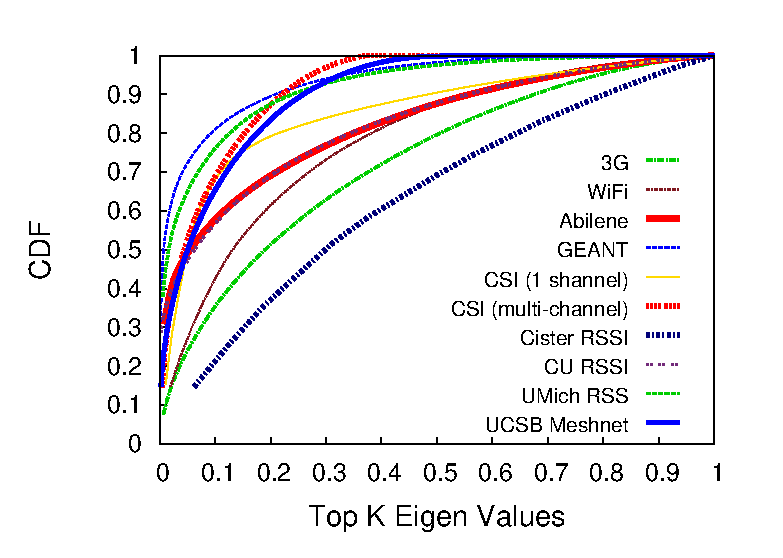
\includegraphics[width=\figurewidthA]{fig/matrix.na0.anom0.rank.eps}
  % \caption{CDF of energy that are contained in the top K singular values
  %   of the original matrices.}
  \caption{CDF of ranks.}
  \label{fig:original-matrix-rank}
\end{figure}

\subsection{Analysis}
\label{ssec:analysis}

\para{Rank analysis:} For each network matrix, we mean center each row (\ie, subtract from
each row its mean value).  We then apply singular value decomposition
(SVD) to examine if the mean-centered matrix has a good low-rank
approximation.  The metric we use is the fraction of total variance
captured by the top $K$ singular values, \ie, $\left({\sum_{i=1}^{K}
  s_i^2}\right)/\left({\sum_{i} s_i^2}\right)$, where $s_i$ is the
$i$-th largest singular value and $\left({\sum_{i} s_i^2}\right)$
gives the total variance of the mean-centered coordinate matrix.  Note
that $1 - \left({\sum_{i=1}^{K} s_i^2}\right)/\left({\sum_{i}
  s_i^2}\right)$ is the relative approximation error of the best
rank-$K$ approximation with respect to the squared Frobenius norm.

Figure~\ref{fig:original-matrix-rank} plots the fraction of total
variance captured by the top $K$ singular values for different
traces. 
As it shows,
% some matrices are low rank. For example, 
% G\'{E}ANT takes 20.8\% singular values to capture 90\%
% variance in the original matrices. 
% However, there are also some matrices are not low rank. 3G 
% and Cister RSSI matrices take 68.1\% and 81.0\% singular values to
% capture 90\% variance respectively.
% We further inject anomalies to see how it affects the results. 
% These results show XXX
from low to high, UCSB Meshnet, G\'{E}ANT, multi-channel CSI, UMich RSS, RON, 
1-channel CSI, CU RSSI, Abilene, WiFi, 3G, and Cister RSSI
matrices take 7.5\%, 20.8\%, 22.0\%, 23.9\%, 47.2\%, 
48.9\%, 55.8\%, 57.0\%, 58.0\%, 68.1\%, and 81.0\%
singular values to capture 90\% variance, respectively. Therefore,
only UCSB Meshnet, G\'{E}ANT, multi-channel CSI, and UMich RSS are
close to low rank.

\begin{figure}[h!]
  \centering
  \subfigure[\small{5\% anomalies with s=0.5}]{
    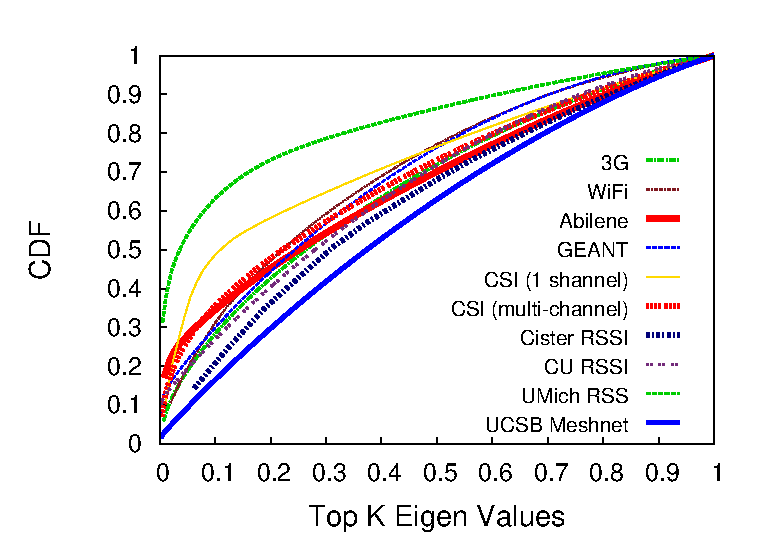
\includegraphics[width=\figurewidthB]{fig/matrix.na0.05.anom0.5.rank.eps}
  }
  \subfigure[\small{10\% anomalies with s=0.5}]{
    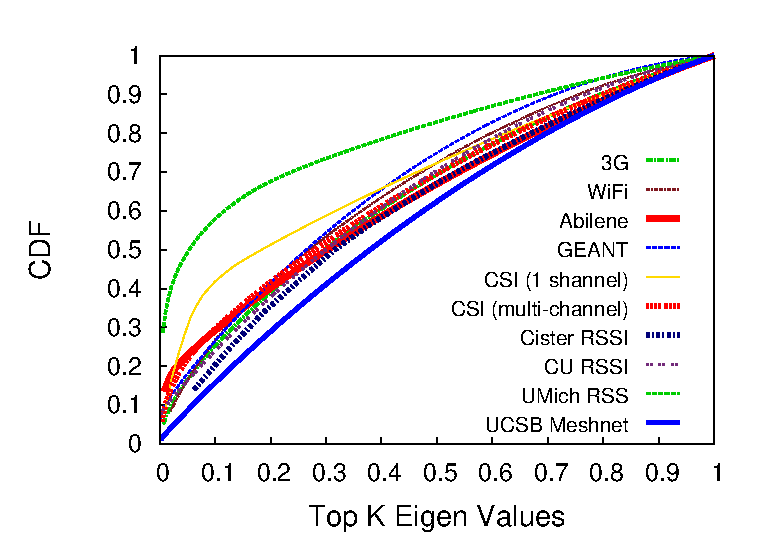
\includegraphics[width=\figurewidthB]{fig/matrix.na0.1.anom0.5.rank.eps}
  }
  \subfigure[\small{5\% anomalies with s=1}]{
    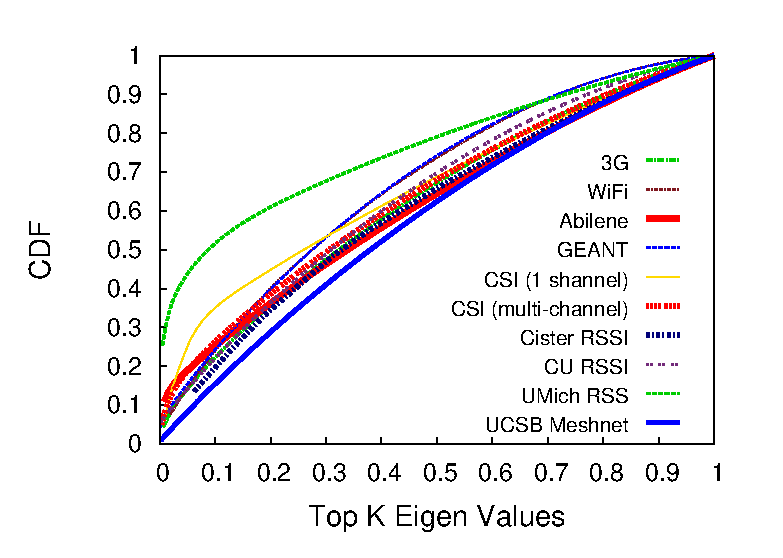
\includegraphics[width=\figurewidthB]{fig/matrix.na0.05.anom1.rank.eps}
  }
  \subfigure[\small{10\% anomalies with s=1}]{
    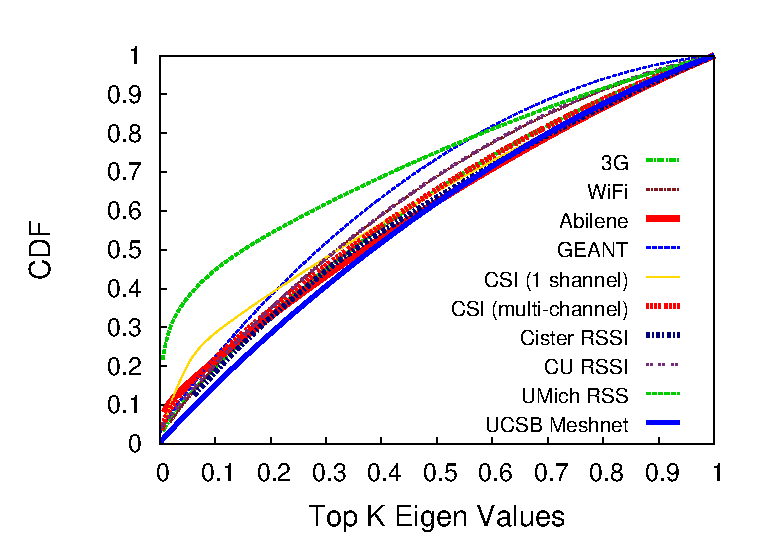
\includegraphics[width=\figurewidthB]{fig/matrix.na0.1.anom1.rank.eps}
  }
  \caption{Ranks under anomalies in traffic matrices.}
  \label{fig:anomalous-traffic-matrix-rank}
\end{figure}

%[also update numbers. Pick a couple of wireless traces instead of
%  Geant to focus on.]  
Next we inject anomalies to see how it affects
the results.  We inject anomalies to a portion of the entries in the
original matrices. Following the standard anomaly injection method
used in existing work~\cite{PCA2, decentralized_PCA, P3CA}, 
we first use exponential weighted
moving average (EWMA) to predict the future entries based on their
past values (\ie, $y=\alpha x + (1-\alpha)y$, where $\alpha=0.8$ in
our evaluation) and use the maximum difference between the actual and
predicted value as the anomaly size to be injected. We vary the
fraction of entries to inject anomalies from 5\% to 10\%, and also
scale the anomaly size by $s$, which is 0.5 or 1. As shown in
Figure~\ref{fig:anomalous-traffic-matrix-rank}, 
% For Abilene, G\'{E}ANT, 3G, and WiFi traffic matrices and RON delay
% matrices, we first normalize each matrix by dividing each entry by the
% maximum element in the matrix. We then inject anomalies by adding or
% subtracting (with equal probability) a number randomly drawn from a
% uniform distribution between $(s,2s)$. We then ensure all entries are
% no smaller than 0 after injecting anomalies, since traffic and delay
% matrices take non-negative values. We vary $s$ and the number of
% entries to which anomalies are injected.
% For convenience, we call $x$ as anomaly size.
when we inject more anomalies or larger anomalies, more singular values are
required in order to capture the variance of the matrices. This trend
is consistent across all traces. For example, as shown in
Figure~\ref{fig:anomalous-traffic-matrix-rank}(a)-(b), 
when we inject 5\% and 10\% anomalies with s=0.5, it takes 60.9\% and
67.6\% singular values to capture 90\% variance in UMich Meshnet, 
71.0\% and 75.8\% in WiFi trace, and 75.7\% and 80.0\% in 1-channel CSI trace.
As shown in
Figure~\ref{fig:anomalous-traffic-matrix-rank}(c)-(d), 
when we inject 5\% and 10\% anomalies with s=1, the corresponding numbers
are 72.5\% and 76.9\% in UMich Meshnet, 72.0\% and 78.3\% in WiFi trace,
and 81.7\% and 84.1\% in 1-channel CSI trace.
% Similarly, but not shown for
% brevity, it takes 79.3\% and 81.8\% singular values for Abilene to
% capture 90\% variance, when we inject 5\% and 10\% anomalies with an
% average size of 0.1, respectively.  The corresponding numbers rose to
% 85.1\% and 86.0\% when we inject 5\% and 10\% anomalies with an
% average size of 0.5, respectively.
The other matrices exhibit the same trend.

% \begin{figure}[h!]
%   \centering
%   \hspace{-0.2in}
%   \subfigure[\small{5\% anomalies with k=1}]{
%     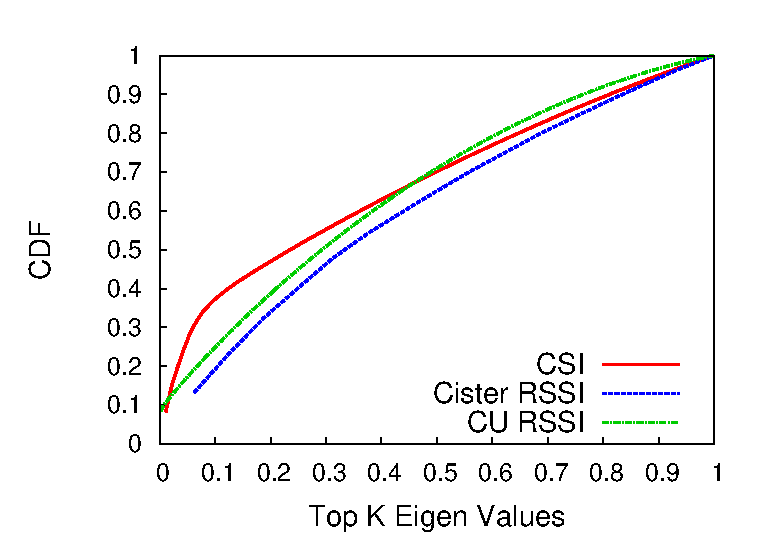
\includegraphics[width=1.0\figurewidthA]{fig/matrix.na0.05.anom2.rank.eps}
%   }
%   \hspace{-0.2in}
%   \subfigure[\small{10\% anomalies with k=1}]{
%     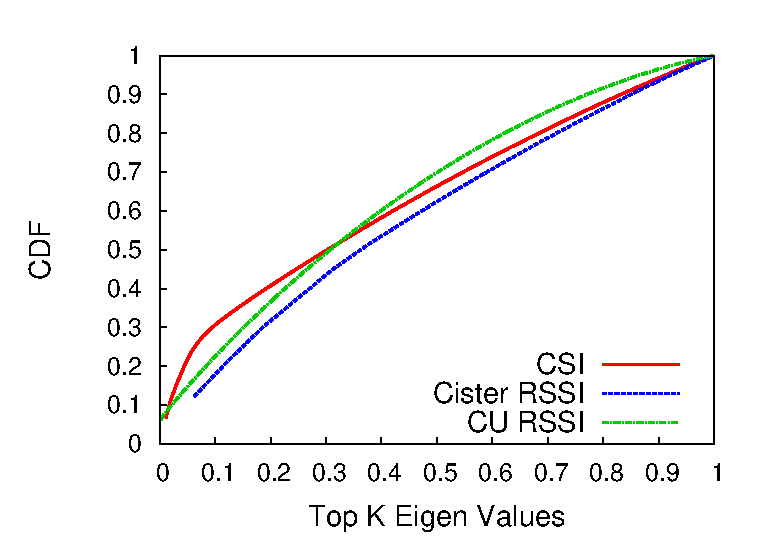
\includegraphics[width=1.0\figurewidthA]{fig/matrix.na0.1.anom2.rank.eps}
%   }
%   \hspace{-0.2in}
%   \subfigure[\small{5\% anomalies with k=2}]{
%     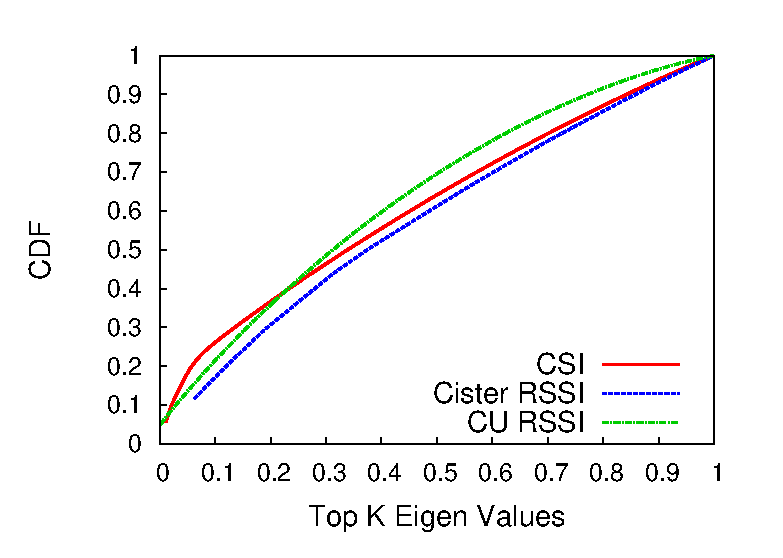
\includegraphics[width=0.99\figurewidthA]{fig/matrix.na0.05.anom4.rank.eps}
%   }
%   \hspace{-0.2in}
%   \subfigure[\small{10\% anomalies with k=2}]{
%     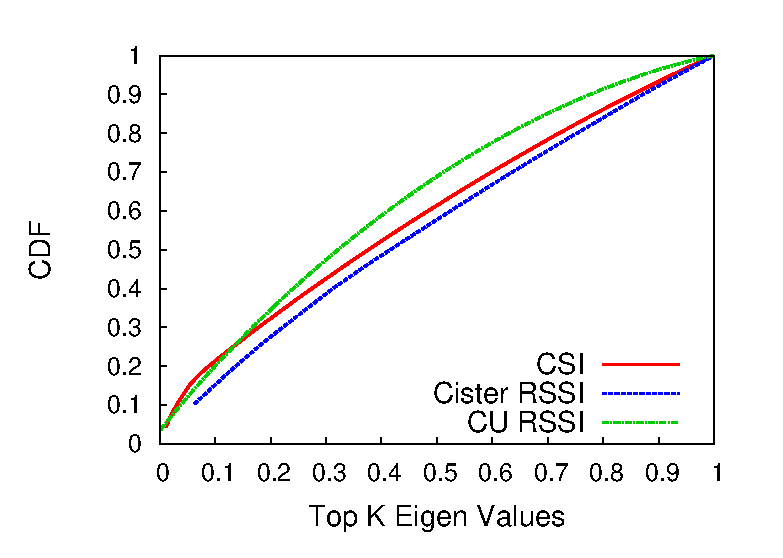
\includegraphics[width=0.99\figurewidthA]{fig/matrix.na0.1.anom4.rank.eps}
%   }
%   \vspace{-0.1in}
%   \caption{CDF of energy that are contained in the top K singular values
%     under anomalies in CSI and RSSI traces.}
%   \vspace{-0.1in}
%   \label{fig:anomalous-rssi-matrix-rank}
% \end{figure}

% We also inject anomalies to SNR and RSS traces. Since the elements in
% SNR and RSS traces have dB as a unit, we use a different way of
% injecting anomalies. We inject anomalies by adding or subtracting a
% number randomly drawn from a uniform distribution between $(k*std,
% 2k*std)$, where $std$ is standard deviation of all elements in a
% matrix. Figure~\ref{fig:anomalous-rssi-matrix-rank} shows the results
% for k=1 and 2. Again we observe the same trend -- the presence of more
% anomalies and larger anomalies increases the rank of the matrix.

\begin{figure}[h!]
  \centering
  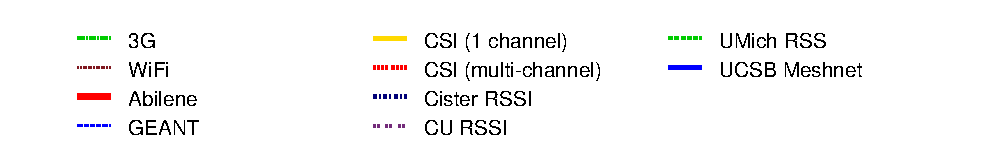
\includegraphics[width=1\columnwidth]{fig/legend_temporal.eps}
  \subfigure[\small{k=1}]{
    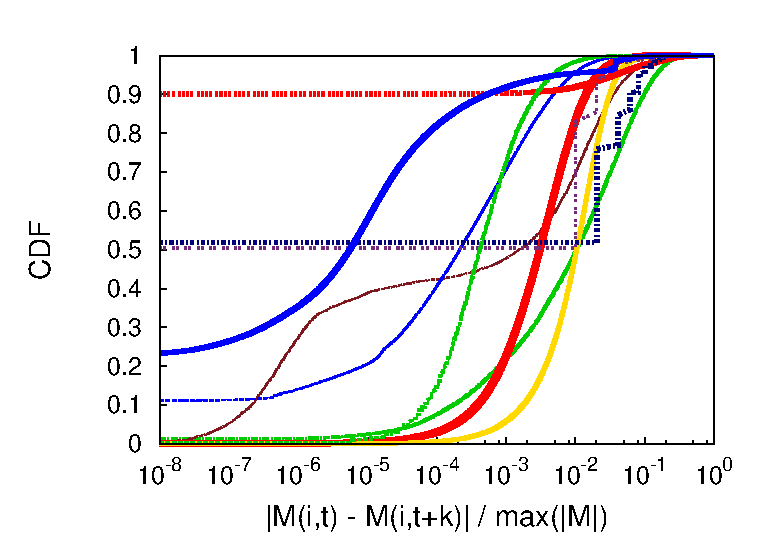
\includegraphics[width=\figurewidthB]{fig/matrix.na0.anom0.itvl1.diff.eps}
  }
  \subfigure[\small{k=10}]{
    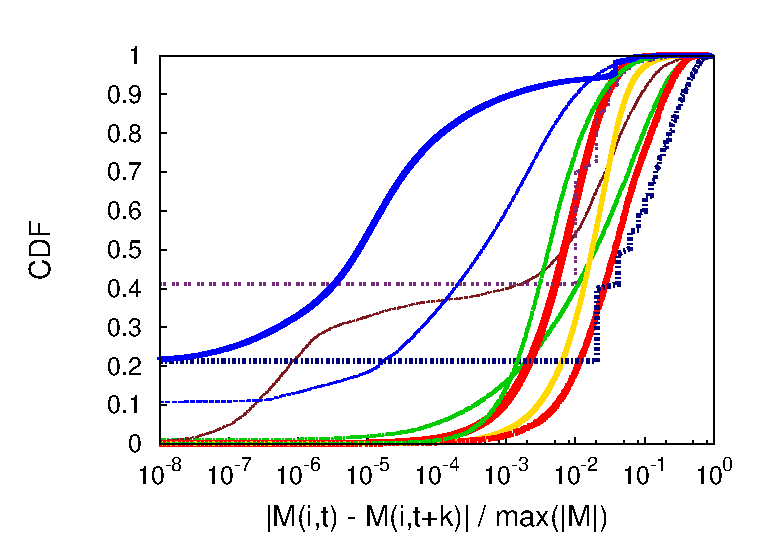
\includegraphics[width=\figurewidthB]{fig/matrix.na0.anom0.itvl10.diff.eps}
  }
  % \caption{CDF of normalized difference between i-th and i+k-th time slot.}
  \caption{CDF of normalized difference between time slots.}
  \label{fig:temporal-stability}
\end{figure}


\para{Temporal stability:} Figure~\ref{fig:temporal-stability} plots the CDF of
normalized temporal variation (\ie, $\frac{x(i)-x(i-t)}{max(x(i))}$)
across different traces. As it shows, different traces exhibit
varying degrees of temporal stability. For example, 3G and Cister RSSI have
high variation: the two adjacent entries differ by 6.1\%-9.8\% in 90\%
cases, and 10 time-slot apart entries differ by 16.7\%-36.2\% in 90\%. 
In comparison, UMich Meshnet and G\'{E}ANT have low variation, where the adjacent
entries differ by 0.3\%-0.5\% in 90\% cases and 10 time-slot apart
entries differ by 1.0\%-2.4\% in 90\%. The other traces are in between.

\para{Summary:} The major findings from the above analysis include: (i) Not
all real network matrices are low rank. (ii) Adding anomalies further
increases the rank. (iii) Temporal stability varies substantially
across different traces. These findings motivate us to develop a
general compressive sensing framework to support diverse matrices that
may not be low rank, exhibit different degrees of temporal stability,
and may even contain anomalies.


%% =================================================================

\section{LENS Decomposition}
\label{sec:lens}

In this section, we first present LENS decomposition framework. Next we develop
an alternating direction method for solving the decomposition
problem. Then we describe how to set the parameters.

\subsection{LENS Decomposition Framework}
\label{ssec:lens}

\para{Overview:} There are many factors that contribute to
real network matrices, including measurement errors, anomalies and
inherent noise.  To capture this insight, we decompose the
original matrix into a {\underline L}ow-rank component, an
{\underline E}rror component, a {\underline N}oise component, and a
{\underline S}parse anomaly component (hence the acronym
{\underline{LENS}} decomposition). This is motivated by the following
observations:
\begin{sitemize}
\item Low-rank component: Network matrices often exhibit significant redundancy.
A concrete form of redundancy is that the network matrix of interest
can be well approximated by low-rank matrices.  For example, TM
estimation makes use of the gravity model~\cite{ZRDG03}, which is
essentially a rank-1
approximation to matrices. \cite{mobile-localization}
uses low-rank matrices for localization.
\item Sparse component: Anomalies are common in large network dataset.
  Anomalies may arise from a number of factors. For example,
  traffic anomalies may be caused by problems ranging from security
  threats (\eg, Distributed Denial of Service (DDoS) attacks and
  network worms) to unusual traffic events (\eg, flash crowds), to
  vendor implementation bugs, and to network misconfigurations.  Such
  anomalies are typically not known a priori and are sparse~\cite{anomaly_sparsity, anomaly_sparsity2}.


Note that there can be systematic effects that are only
sparse after some transformation (\eg, wavelet transform).  For
example, a major level shift may result in persistent changes in the
original data (and is thus not sparse).  But after wavelet transform
(or simple temporal differencing), it becomes sparse. 

\item Error and artifacts: The measurement and data collection procedure
may also introduce artifacts. For example, a SNMP traffic counter may wrap
around, resulting in negative measurements.
One can always try his best to apply domain knowledge to filter out
obvious errors and artifacts (\eg, missing data or negative traffic
measurements).  However, in general it is difficult to filter out all
such artifacts.  The advantage of considering both anomalies and
errors jointly is that the parts that cannot be filtered can get
absorbed by the sparse components.

\item Noise.  Noise is universal, making clean mathematical models
approximate in practice. For example, real-world network matrices are
typically only approximately low-rank as opposed to exactly low-rank.

%\item Locality. Network data may also exhibit spatial or temporal
%locality \cite{anomaly_spatio_temporal,Wang:2002:model_spatio_temporal,
% George:2007:spatio_temporal_database}. 
% For example, traffic 
% at similar point of time may be similar. 
% Temperature at similar locations are similar.
\end{sitemize}


% Considering all these effects.
Therefore a natural approach is to consider the
original dataset as a mixture of all these effects.  It is useful if
one can decompose the original matrix into individual components, each
component capturing one major effect.

\para{Basic formulation:} The basic LENS decomposition decomposes an original $m\times n$ data matrix $D$ into
a low-rank matrix $X$, a sparse anomaly matrix $Y$, a noise matrix
$Z$, and an error matrix $W$.  This is achieved by solving the
following {\em convex} optimization problem:
\begin{eqnarray}
\text{minimize:} && \alpha \|X\|_* + \beta \|Y\|_1 + 
                    \frac{1}{2\sigma}\|Z\|_F^2, \nonumber\\
\text{subject to:}&& X + Y + Z + W = D, \nonumber\\
&& E.*W = W.
\label{eq:lens-basic}
\end{eqnarray}
where $X$ is a low-rank component, $Y$ is a sparse anomaly component,
$Z$ is a dense noise term, and $E$ is a binary error indicator matrix
such that $E[i,j] = 1$ if and only if entry $D[i,j]$ is erroneous or
missing, and $W$ is an arbitrary error component with $W[i,j] \neq 0$
only when $E[i,j] = 1$ (thus $E.*W = W$, where $.*$ is an element-wise
multiplication operator). Since $W$ fully captures the erroneous or
missing values, we can set $D[i,j] = 0$ whenever $E[i,j] = 1$ without
loss of generality. The constraint enforces $D$ to be the sum of $X$,
$Y$, and $Z$ when $D$ is neither missing nor has errors (since
$E[i,j].*W[i,j] = 0$ in this case), while imposing no constraint when
$D$ is missing or has error (since $E[i,j].*W[i,j]=W[i,j]$ allows
$W[i,j]$ to take an arbitrary value to satisfy $X+Y+Z+W=D$).

The optimization objective has the following three components:
\squishlist
\item $\|X\|_*$ is the nuclear norm~\cite{recht08:_nec,recht:_guaran} of
  matrix $X$, which penalizes against high rank of $X$ and can be
  computed as the total sum of $X$'s singular values.

\item $\|Y\|_1$ is the $\ell_1$-norm of $Y$, which penalizes against
  lack of sparsity in $Y$ and can be computed as $\|Y\|_1 = \sum_{i,j}
  |Y[i,j]|$.

\item $\|Z\|_F^2$ is the squared Frobenius norm of matrix $Z$, which
penalizes against large entries in the noise matrix $Z$ and can be computed as
$\|Z\|_F^2 = \sum_{i,j} Z[i,j]^2$.

\squishend

The weights $\alpha$, $\beta$ and $\frac{1}{2\sigma}$ balance the
conflicting goals to simultaneously minimize $\|X\|_*$, $\|Y\|_1$ and
$\|Z\|_F^2$.  We describe how to choose these weights in
Section~\ref{ssec:para}.  


\para{Generalized formulation:} Below we generalize both the
constraints and the optimization objective of the basic formulation in
Eq.~\eqref{eq:lens-basic} to accommodate rich requirements in the
analysis of real-world network matrices.

%\begin{sitemize}
  
%\item
First, the matrix of interest may not always be directly observable,
  but its linear transform can be observed though subject to missing
  data, measurement errors, and anomalies. For example, end-to-end
  traffic matrices $X$ are often not directly observed, and what can
  be observed are link load $D$. $X$ and $D$ follow $AX = D$, where
  $A$ is a binary routing matrix: $A(i,j) =
  1$ if link $i$ is used to route traffic for the $j$-th end-to-end
  flow, and $A(i,j) = 0$ otherwise.  We generalize the constraints in
  Eq.~\eqref{eq:lens-basic} to cope with such measurement
  requirements:
\begin{equation}
 AX + BY + CZ + W = D
\end{equation}
Here $A$ may capture tomographic constraints that linearly relate
direct and indirect measurements (\eg, 
$A$ is a routing matrix in the traffic matrices).  $B$ may represent an over-complete anomaly
profile matrix. If we do not know which matrix entries may have
anomalies, we can simply set $B$ to the identity matrix $I$. It is also
possible to set $B=A$ if we are interested in capturing anomalies in
$X$.  Without prior knowledge, we set $C$ to be the identity
matrix.



Prior research on network inference and compressive sensing
  highlights the importance of incorporating domain knowledge about
  the structure of the underlying data. To capture domain knowledge,
  we introduce one or more penalty terms into the
  optimization objective: $\sum_{k=1}^K \|P_k X Q_k^T - R_k\|_F^2$,
  where $K$ is the number of penalty terms.  We also introduce a
  weight $\gamma$ to capture our confidence in such knowledge.

Examples of domain knowledge include temporal stability constraints,
spatial locality constraints, and initial estimation of $X$ (\eg,
\cite{ZRDG03} derives initial traffic matrices using the gravity
model~\cite{gravity1}). Temporal and spatial locality are common 
in network data~\cite{anomaly_spatio_temporal,Wang:2002:model_spatio_temporal,George:2007:spatio_temporal_database}. Such domain knowledge is especially helpfulwhen there are many missing entries, making the problem severely
under-constrained.
%locality . 
% For example, traffic 
% at similar point of time may be similar. 
% Temperature at similar locations are similar.

Consider a few simple cases. First, when
$k=1$, $P_1$ is an identity matrix $I$, $R_1$ is a zero vector, we can
set $Q_1=Toeplitz(0,1,-1)$, which denotes the Toeplitz matrix with
central diagonal given by ones, the first upper diagonal given by
negative one, \ie,
\begin{equation}
  Q = \left[
   \begin{array}{rrrrrrrr}
         1 & -1 &  0 &  0 &  \ldots \\
         0 &  1 & -1 &  0 & \ddots \\
         0 &  0 &  1 & -1 & \ddots \\
         \vdots &  \ddots &  \ddots & \ddots &  \ddots   \\
   \end{array} \right].
\end{equation}
$Q^T$ denotes the transpose of matrix $Q$. $P_1 X Q_1^T$ captures the
differences between two temporally adjacent elements in
$X$. Minimizing $\|P_1 X Q_1^T - R_1\|_F^2=\|P_1 X Q_1^T\|_F^2$
reflects the goal of making $X$ temporally stable. For simplicity,
this is what we use for our evaluation. In general, one can use
similar constraints to capture other temporal locality patterns during
different periods (\eg, seasonal patterns or diurnal patterns).

Next we consider the spatial locality, which is represented by $P$. If
$k=1$, $R_1=0$, $Q_1$ is an identity matrix $I$, we can set $P_1$ to
reflect the spatial locality. For example, if two adjacent elements in
the matrix have similar values, we can set $P =
Toeplitz(0,1,-1)$. Similarly, if different parts of the matrix have
different spatial locality patterns, we can use different $P$'s to
capture these spatial locality patterns. For simplicity, our
evaluation considers only temporal stability, which is well known to
exist in different networks. We plan to incorporate spatial locality
in the future.

% We also selectively evaluate the spatial locality
% on some matrices that are likely to exhibit locality (\eg, CSI
% matrices where SNR on adjacent frequencies should be similar).

Finally, if we have good initial estimate of $X_{init}$ (\eg, \cite{ZRDG03}
uses the gravity model to derive the initial TM), we can
leverage this domain knowledge by minimizing $\|X - X_{init}\|$ (\ie, $R_1=X_{init}$). This
term can be further combined with spatial and/or temporal locality to
produce richer constraints.

%\end{sitemize}  

Putting everything together, the general formulation is:

{\small
\begin{eqnarray}
\text{minimize:}  && \alpha \|X\|_* + \beta \|Y\|_1 +
\frac{1}{2\sigma}\|Z\|_F^2 +\frac{\gamma}{2\sigma}\sum_{k=1}^K\|P_k X Q_k^T - R_k\|_F^2, \nonumber\\
\text{subject to:}&& AX + BY + CZ + W = D, \nonumber\\
&& E.*W = W.
\label{eq:general-lens-basic}
\end{eqnarray}
}
Note that our formulation is more general than recent research on
compressive sensing
(\eg,~\cite{zhang09sensing,robustPCA,recht08:_nec,recht:_guaran}),
which do not consider anomalies,
% (typically only 2 or 3 components out of $\{X,Y,Z,W\}$),
have simpler constraints (\eg, there is no
$A$, $B$, or $C$), and have less general objectives.

% XXX  For example, to
% enumerate all possible spike locations, we can simply set $B$ to be
% the identity matrix $I$.  % Alternatively, $B$ can also be constructed
% using Haar wavelet transform matrix, or the discrete cosine transform
% matrix, or a combination of these.
% We ensure that columns of $B$ are
% distinct and have unit length. % $C$ is XXX.

%In this case, we observe that (i) when $X$ is low-rank, $AX$ is also
%low-rank, and (ii) when $Z$ is a dense noise matrix, $CZ$ is also
%likely to be dense.  We therefore propose to infer $X$, $Y$, $Z$, and
%$W$ by solving
%\begin{eqnarray}
%\text{minimize:}  && \alpha \|AX\|_* + \beta \|Y\|_1 
%                    +\frac{1}{2\sigma}(\|T*Q^T\|_F^2+\|CZ\|_F^2), \nonumber\\
%\text{subject to:}&& AX + BY + T + CZ + E.*W = D, \label{eq:lens-general}
%\end{eqnarray}  
%where $\sigma$ becomes the standard deviation of (non-erroneous)
%elements of $CZ$ instead of $Z$.

\subsection{Optimization Algorithm}
\label{ssec:adm}

The generality of the formulation in Eq.~\eqref{eq:general-lens-basic}
makes it challenging to optimize. We are not aware of any
existing work on compressive sensing that can cope with such a general
formulation.  Below we first reformulate
Eq.~\eqref{eq:general-lens-basic} to make it easier to solve.  We then
consider the augmented Lagrangian function of the reformulated problem
and develop an Alternating Direction Method to solve it.

\para{Reformulation for optimization:} Note that $X$ and $Y$ appear in
multiple locations in the objective function and constraints in the
optimization problem~\ref{eq:general-lens-basic}. This coupling makes
optimization difficult. To reduce coupling, we introduce a set of
auxiliary variables $X_0,X_1,\cdots,X_{K}$ and $Y_0$ and reformulate
the problem as follows:
\begin{eqnarray}
\text{minimize:}  && \alpha \|X\|_* + \beta \|Y\|_1 +
\frac{1}{2\sigma}\|Z\|_F^2 \nonumber\\
                  && \quad+\frac{\gamma}{2\sigma}\sum_{k=1}^K\|P_k X_k Q_k^T - R_k\|_F^2, \nonumber\\
\text{subject to:}&& AX_0 + BY_0 + CZ + W = D, \nonumber\\
&& E.*W = W, \nonumber\\
&& X_k - X = 0\quad (\forall k=0,\cdots,K\nonumber),\\
&& Y_0 - Y = 0.
\label{eq:reformulated-lens}
\end{eqnarray}
where $Y_0$ and $X_{k} (0\leq k \leq K)$ are auxiliary variables.
Note that formulations Eq.~\eqref{eq:reformulated-lens} and
Eq.~\eqref{eq:general-lens-basic} are equivalent.

\comment{ %old lens
Note that we can simplify Eq.~\eqref{eq:lens-general} by performing a
change of variable.  Specifically, let $X = A X_{\mathrm{orig}}$ and
$Z = C Z_{\mathrm{orig}}$, then Eq.~\eqref{eq:lens-general} becomes:
\begin{eqnarray}
\text{minimize:}  && \alpha \|X\|_* + \beta \|Y\|_1 +
                     \frac{1}{2\sigma}(\|T*Q^T\|_F^2 + \|Z\|_F^2), \nonumber\\
\text{subject to:}&& X + BY + T + Z + E.*W = D. \label{eq:lens-simple}
\end{eqnarray}  

Once we solve Eq.~\eqref{eq:lens-simple}, we can then infer
$X_{\mathrm{orig}}$ and $Z_{\mathrm{orig}}$ according to
$X_{\mathrm{orig}} = \mathsf{pinv}(A) X$ and $Z_{\mathrm{orig}} =
\mathsf{pinv}(C) Z$, where $\mathsf{pinv}(M)$ is the pseudo-inverse
of matrix $M$.  
}

\para{Alternating Direction Method for solving
  \eqref{eq:reformulated-lens}:} We apply an Alternating Direction
Method (ADM)~\cite{adm} to solve the convex optimization problem in
~\eqref{eq:reformulated-lens}.  Specifically, we consider the
augmented Lagrangian function:

\begin{small}
\begin{eqnarray}
\lefteqn{\mathcal{L}(X,\{X_k\},Y,Y_0,Z,W,M,\{M_k\},N,\mu)}\nonumber\\
\defas&&\alpha\|X\|_* + \beta\|Y\|_1 + \frac{1}{2\sigma}\|Z\|_F^2\nonumber\\
&&   +~ \frac{\gamma}{2\sigma} \sum_{k=1}^K \|P_k X_k Q_k^T-R_k\|_F^2\nonumber\\
&&   +~ \langle M,D-AX_0-BY_0-CZ-W \rangle \label{eq:lang1}\\ 
&&   +~ \sum_{k=0}^K\langle M_k,X_k-X\rangle \label{eq:lang2}\\
&&   +~ \langle N,Y_0-Y \rangle \label{eq:lang3}\\
&&   +~ \frac{\mu}{2}\cdot \|D-AX_0-BY_0-CZ-W\|_F^2 \label{eq:penalty1}\\
&&   +~ \frac{\mu}{2}\cdot \sum_{k=0}^K \|X_k-X\|_F^2 \label{eq:penalty2}\\
&&   +~ \frac{\mu}{2}\cdot \|Y_0-Y\|_F^2 \label{eq:penalty3}
\end{eqnarray}
\end{small}
where $M$, $\{M_k\}$, $N$ are the Lagrangian
multipliers~\cite{lag-multiplier} for the equality constraints in
Eq.~\eqref{eq:reformulated-lens}, and $\langle U, V\rangle \defas
\sum_{i,j} (U[i,j] \cdot V[i,j])$ for two matrices $U$ and $V$ (of the
same size).  Essentially, the augmented Lagrangian function includes
the original objective, three Lagrange multiplier terms
\eqref{eq:lang1}--\eqref{eq:lang3}, and three penalty terms converted
from the equality constraints
\eqref{eq:penalty1}--\eqref{eq:penalty3}.  Lagrange multipliers are
commonly used to convert an optimization problem with equality
constraints into an unconstrained one.  Specifically, for any optimal
solution that minimizes the (augmented) Lagrangian function, the
partial derivatives with respect to the Lagrange multipliers must be
0.  Hence the original equality constraints will be satisfied.  The
penalty terms enforce the constraints to be satisfied.  The benefit of
including Lagrange multiplier terms in addition to the penalty terms
is that $\mu$ no longer needs to iteratively increase to $\infty$ to
solve the original constrained problem, thereby avoiding
ill-conditioning~\cite{adm}.  Note that we do not include terms
corresponding to constraint $E.*W=W$ in the augmented Lagrangian
function, because it is straightforward to enforce this constraint
during each iteration of the Alternating Direction Method without the
need for introducing additional Lagrange multipliers.

%\begin{eqnarray*}
%&\mathcal{L}(X,Y,Z,W,T,M,\mu) \\
%\defas&\alpha\|X\|_* + \beta|Y|_1 +  \frac{1}{2\sigma} (\|Z\|_F^2 +\|T*Q^T\|_F^%2)  \\
%&+ \langle M, D-X-BY-Z-T-W \rangle \\
%&+ \frac{\mu}{2}\|D-X-BY-Z-T-W\|_F^2,
%\end{eqnarray*}
%where $M$ is the Lagrange multipliers for constraints
%$D-X-BY-Z-T-W=0$, and $\langle M, N\rangle = \sum_{i,j} (M[i,j] \cdot
%N[i,j]) = \mathsf{trace}(M\cdot N)$ is the trace of $M\cdot N$.

The ADM algorithm progresses in an iterative fashion.  During each
iteration, we alternate among the optimization of the augmented
Lagrangian function by varying each one of $X$, $\{X_k\}$, $Y$, $Y_0$,
$Z$, $W$, $M$, $\{M_k\}$, $N$ while fixing the other variables.  
Introducing auxiliary variables $\{X_k\}$ and $Y_0$ makes it
possible to obtain a close-form solution for each optimization
step. Following ADM, 
% The procedure is guaranteed to converge quickly if
we increase $\mu$ by a constant factor $\rho \geq 1$ during each
iteration.  When involving only two components, ADM is guaranteed to
converge quickly.  In our general formulation, convergence is no
longer guaranteed, though empirically we observe quick convergence in
all our experiments (\eg, as shown in Section~\ref{sec:eval}).  We
plan to apply techniques in \cite{convergence} to ensure guaranteed
convergence in future work. We further improve efficiency by
replacing exact optimization with approximate optimization during each
iteration. Appendix~\ref{appendix:adm} gives a detailed description on
the steps during each iteration.

\para{Improving efficiency through approximate SVD:} The most
time-consuming operation during each iteration of the Alternating
Direction Method is performing the singular value decomposition.  In
our implementation, we add an additional constraint on the rank of
matrix $X$: $ rank(X) \leq r$, where $r$ is a user-specified parameter
that represents an estimated upper bound on the true rank of $X$.  We
then explicitly maintain the SVD of $X$ and update it approximately
during each iteration through the help of rank-revealing QR
factorization of matrices that have only $r$ columns (which are much
smaller than the original matrices used in SVD).  We omit the details
of approximate SVD in the interest of space.  % We plan to release our
% Matlab implementation of LENS decomposition after the paper is
% published.
  
\subsection{Setting Parameters}
\label{ssec:para}

\para{Setting $\alpha$, $\beta$ and $\sigma$:} A major advantage of
our LENS decomposition is that a good choice of the parameters
$\alpha$ and $\beta$ can be analytically determined without requiring
any manual tuning.  Specifically, let $\sigma_D$ be the standard
deviation of measurement noise in data matrix $D$ (excluding the
effect of low-rank, sparse, and error terms).  For now, we assume that
$\sigma_D$ is known, and we will describe how to determine $\sigma_D$
later in this section. Moreover, we first ignore the domain knowledge
term and will adaptively set $\gamma$ for the domain knowledge term
based on the given $\alpha$ and $\beta$.

Let density $\eta(D) = 1 - \frac{\sum_{i,j} E[i,j]}{m\times n}$ be the
fraction of entries in $D$ that are neither missing nor erroneous,
where the size of $D$ is $m \times n$ and the size of $Y$ is
$m_Y\times n_Y$. $E[i,j]$ can be estimated based on domain knowledge.
For example, we set $E[i,j]=1$ if the corresponding entry takes a value outside
its normal range (\eg, a negative traffic counter) or measurement
software reports an error on the entry. Moreover, our evaluation shows
that LENS is robust against estimation error in $\eta(D)$.

We propose to set:
\begin{eqnarray}
\alpha &=& (\sqrt{m_X}+\sqrt{n_X})\cdot \sqrt{\eta(D)} \label{eq:alpha}\\
\beta  &=& \sqrt{ 2\cdot \log(m_Y\cdot
  n_Y)} \label{eq:beta}\\
\sigma &=& \theta \cdot \sigma_D \label{eq:sigma}
\end{eqnarray}
where $(m_X,n_X)$ is the size of $X$, $(m_Y,n_Y)$ is the size of $Y$.
$\theta$ is a user-specified control parameter that limits the
contamination of the dense measurement noise $\sigma_D$ when computing
$X$ and $Y$.  In all our experiments, we set $\theta = 10$,
though it is also possible to choose $\theta$ adaptively, just like
how we choose $\gamma$ as described later in this section.

Below we provide some intuition behind the above choices of $\alpha$
and $\beta$ using the basic formulation in
Eq.~\eqref{eq:lens-basic}. The basic strategy is to consider all
variables except one are fixed.
% the special case where
% among the three components $X$, $Y$, $Z$ only two components are
% present.
Our evaluation shows that these choices work well in
practice.  

\para{Intuition behind the choice of $\alpha$:} 
Consider the special case when all variables except that $X$ are already
given and stay 
fixed. Then we just need to solve: % [XXX: why solve this]
\begin{equation}
\min_{X}\quad \alpha\cdot\|X\|_* +
\frac{1}{2\sigma}\cdot\|D-X-Y-W\|_F^2
\label{eq:opt-X}
\end{equation}
since $Z=D-X-Y-W$.
We can prove the optimal $X$ in Eq.~\eqref{eq:opt-X} can be
% We search for $X$ in Eq.~\eqref{eq:opt-X}
obtained by performing soft-thresholding (a.k.a., shrinkage) on the
singular values of $D-Y-W$.  That is, % Specifically, we have:
\begin{eqnarray}
X_{\mathrm{opt}}& = &\mathsf{SVSoftThresh}(D-Y-W,~\alpha\cdot\sigma)\notag\\
& \defas &U*\mathsf{SoftThresh}(S,~\alpha\cdot\sigma)*V^T,\label{eq:X_opt}
\end{eqnarray}
where $[U,S,V] = \mathsf{svd}(D-Y-W)$ is the singular value
decomposition of $(D-Y-W)$ (thus $D-Y-W = U S V^T$), and
$\mathsf{SoftThresh}(S,~\alpha\sigma) = \mathsf{sign}(S) .*
\max\{0,~\mathsf{abs}(S)-\alpha\sigma\}$ ($\mathsf{sign}(S) =
S./\mathrm{abs}(S)$).  Intuitively, soft-thresholding eliminates the
contamination on the singular values of $X$ due to the dense
measurement noise $\sigma_D$.

From asymptotic random matrix theory~\cite{dneedell07norm}, for a
random matrix with entries drawn $i.i.d.$ from a Gaussian distribution
with probability $\eta(D)$, its norm (\ie, the largest singular value)
is bounded by $O((\sqrt{m}+\sqrt{n})\cdot\sqrt{\eta(D)}\cdot\sigma_D)$
with a high probability.  So a good heuristic is to set the soft
threshold to:
\[
\alpha\cdot\sigma =
(\sqrt{m}+\sqrt{n})\cdot\sqrt{\eta(D)}\cdot\sigma_D \cdot \theta,
\]
where $\theta$ is a control parameter that captures the desired
separation from the influence of dense measurement noise $\sigma_D$.
Therefore, we simply set
$\alpha=(\sqrt{m}+\sqrt{n})\cdot\sqrt{\eta(D)}$ and $\sigma=\theta
\cdot\sigma_D$.
\comment{
Note that in reality $D-X-Y-W$ consists of a mixture of the measurement
noise, and the residual noise introduced by applying
$\mathsf{SVSoftThresh}$ for $X$ and $\mathsf{SoftThresh}$ for $Y$ (see
below).  As a result, even when the measurement noise $Z$ may not be
strictly Gaussian, $D-X-Y-W$ is likely to be Gaussian-like. This is
similar to Principal Component Analysis whose residuals tend to be
Gaussian like).}

\para{Intuition behind the choice of $\beta$:}
Now suppose $X$ is given and we need to solve:
\begin{equation}
\min_Y\quad \beta\dot\|Y\|_1 + \frac{1}{2\sigma}\cdot \|D-X-Y-W\|_F^2 
\label{eq:opt-Y}
\end{equation}

We can prove that the optimal $Y$ for \eqref{eq:opt-Y} can be
obtained by performing soft-thresholding (a.k.a., shrinkage) on the
entries of $D-X-W$. Specifically, we have:
\begin{equation}
Y_{\mathrm{opt}} = \mathsf{SoftThresh}(D-X-W,~\beta\cdot\sigma),
\label{eq:Y_opt}
\end{equation}
where soft-thresholding eliminates the contamination on entries of $Y$
due to the dense measurement noise.

In the context of standard compressive sensing setting:
\[
\min_y\quad \beta*\sigma_d\cdot\|y\|_1 + \frac{1}{2}\cdot\|y-d\|_2^2,
\]
where $y$ is a vector of length $n_y$, and $\sigma_d$ is the standard
deviation of the vector of observables $d$. As justified in Basis
Pursuit De-Noising (BPDN)~\cite{Chen98atomicdecomposition}, a penalty
term $\beta = \sqrt{2\cdot \log(n_y)}$ should be used, where $n_y$ is
the number of elements in $Y$.  Similarly, in our context, a good
heuristic is to set the soft threshold to:
\[
\beta\cdot \sigma = \sqrt{2\cdot\log(m_Y\cdot n_Y)}\cdot\sigma_D\cdot\theta.
\]
So we simply set $\beta=\sqrt{2\cdot\log(m_Y\cdot n_Y)}$ and
$\sigma=\theta \cdot\sigma_D$.

\para{Estimating $\sigma_D$:} When $\sigma_D$ is not known in advance,
we simply estimate it from entries of $D-AX_0-BY_0-W$ during each
iteration in the Alternating Direction Method (see
Appendix~\ref{appendix:adm}). Specifically, let $J=D-AX_0-BY_0-W$, we
estimate $\sigma_D$ as the standard deviation of
$\{J[i,j]~|~E[i,j]=0\}$.  It is also possible to use a more robust
estimator (\eg, the mean absolute value), which gives similar
performance in our experiments.

\para{Searching for $\gamma$:} $\gamma$ reflects the importance of
domain knowledge terms. It is challenging to find an appropriate
$\gamma$, since its value depends on how valuable are the domain
knowledge versus the information from the measurement data. Therefore
instead of using a fixed value, we automatically learn $\gamma$
without user feedback or ground-truth of the real missing entries as
follows. Given the incomplete data matrix $D$, we further drop
additional entries of $D$ and apply our algorithm under several
$\gamma$ values, and quantify the error of fitting the entries that
were present in $D$ but dropped intentionally during the search (so we
know their true values). We adopt the value of $\gamma$ that gives the
lowest fitting error on these entries as the final $\gamma$ and apply
it to our final matrix interpolation, which only has the real missing
elements.

\para{Supporting the general formulation:} In the general formulation
in Eq.~\eqref{eq:general-lens-basic}, we first ensure that matrices
$A$, $B$, $C$ are properly scaled such that each column of $A$, $B$,
$C$ has unit length (i.e. the square sum of all elements in a column
is equal to $1$).  We also automatically scale $P_k$, $Q_k$, $R_k$
such that each row of $P_k$ and $Q_k$ has unit length.  We then use
the same choice of $\alpha$, $\beta$, $\sigma$, and $\gamma$ as in the
basic formulation.

%%%%%%%%%%%%%%%%%%%%%% end of file %%%%%%%%%%%%%%%%%%%%%%%%%%
\comment{
\subsection{Combining LENS with SRMF and KNN}
\label{ssec:combine}

\cite{zhang09sensing} develops a novel {\em spatio-temporal
  compressive sensing} framework with two key components: (i) a new
technique called {\sc Sparsity Regularized Matrix Factorization
  (SRMF)} that leverages the spatio-temporal characteristics of
real-world traffic matrices in addition to their sparse or low-rank
structure, and (ii) a mechanism for combining low-rank approximations
with local interpolation procedures.  % Using a large amount of real
% traffic data collected from three ISP networks (including a tier-1
% ISP),
Using real traffic matrices, the authors show their spatio-temporal compressive sensing significantly
outperforms existing methods and can handle up to 98\% missing values.


% As shown in Section~\ref{sec:eval}, LENS can significantly out-perform
% SRMF+KNN under anomalies. However, when there are no anomalies, LENS
% perform comparably and sometimes slightly worse than SRMF+KNN. This is
% because SRMF+KNN is designed for the cases without anomalies, whereas
% LENS uses a more general formulation to support estimation under
% anomalies and requires estimating additional unknowns (\ie, $Y$ and
% $Z$), which may introduce additional uncertainty and increase errors.
% When the system is under-constrained, the additional unknowns make
% it  which may induce more errors.

% To achieve the best of both worlds, we develop a scheme to leverage
% LENS and SRMF+KNN. First, we use LENS to get initial estimates. 
% if the estimated $Y_{LENS}$ has small magnitude,
% Then we treat all matrix
% entries with nonzero $Y$ as missing values and apply SRMF+KNN~\cite{zhang09sensing} to estimate
% $X_{SRMF}$. Finally we estimate $X = X_{SRMF+KNN}+Y_{LENS}$. As shown
% in Section~\ref{sec:eval}, the combined scheme consistently
% out-performs both LENS and SRMF+KNN.
% We further exploit the
% local structure in the matrix using $K$ nearest neighbors
% (KNN). Specifically, we use a regression to determine weights $w(k)$
% such that $X(r,j) = \sum_{k \in nbrs} w(k) X(r,k)$, and then use the
% estimated weights to get the final $X(i,j) = \sum_{k \in nbrs} w(k)
% X(i,k)$.
Inspired by \cite{zhang09sensing}, we enhance LENS by combining LENS
with KNN and SRMF as follows.
% To achieve the best of both worlds, we develop a scheme to leverage
% LENS+KNN and SRMF+KNN.
\begin{enumerate}
\item We use LENS to get initial estimate $X_{LENS}$.
% Then we subtract the anomalies $Y$ from the estimates and apply
% KNN. Subtracting $Y$ can prevent anomalies 
% from affecting the nearby entries.
\item We then apply KNN to $X_{LENS}$ by first using a regression to learn a set of weights
$w(k)$ that gives the closest approximation to row $r$. That is,
  \[X(r,j) =\sum_{k\in nbrs} w(k) X_{LENS}(r,k)\]
  and then applying the learned weights to perform linear
  interpolation:
  \[X_{LENS+KNN}^{part}(i,j) =\sum_{k\in nbrs}w(k)X_{LENS}(i,k).\] As
  in \cite{zhang09sensing}, we use the adjacent left 3 columns and
  adjacent right 3 columns as neighbors. These columns represent the
  values during the previous and next 3 time intervals.
\item We add $Y$ back to get estimates of LENS+KNN as $X_{LENS+KNN}=X_{LENS+KNN}^{part}+Y$.
\item We treat all matrix entries with nonzero $Y$ as missing values
and apply SRMF+KNN~\cite{zhang09sensing} to estimate $X_{SRMF+KNN}$.
\item We combine $X_{LENS+KNN}$ and $X_{SRMF+KNN}$ to get the final
estimate:
\[{\scriptsize X_{LENS+SRMF+KNN}(i,j)\\
  = \left\{\begin{array}{rr}
X_{LENS+KNN}(i,j) & if\ Y(i,j) \neq 0\\
X_{SRMF+KNN}(i,j) & if\ Y(i,j) = 0\end{array}\right.}\]
\end{enumerate}
% $X_{LENS+SRMF+KNN}(i,j) = X_{SRMF+KNN}(i,j)$ when $Y(i,j)
% = 0$.

% getting entries with nonzero $Y$ from $X_{LENS+KNN}$ and entries with
% zero $Y$ from $X_{SRMF+KNN}$.

The combined algorithm has several desirable properties. First, we
apply KNN to exploit local structure in addition to the global
low-rank and temporal structures. However, unlike SRMF, we remove
anomalies before applying KNN so that we prevent anomalous entries
from contaminating nearby normal entries. Second, SRMF is sufficient
when there are no anomalous or noise, while LENS excels under
anomalies. By combining LENS with SRMF, we achieve the best of both
worlds. 

% we combine LENS with
% SRMF to achieve good performance with and without anomalies since SRMF is effective under no anomalies while LENS excels
% under anomalies. 
% 
% so that we can achieve good performance with and without
% anomalies.
}
%%%%%%%%%%%%%%%%%%%%%%%%%% end of file %%%%%%%%%%%%%%%%%%%%%%%%%%%%
\comment{
\subsubsection{Extensions}

We can further extend LENS decomposition to (i) cope with unknown
noise level $\sigma$, (ii) incorporate spatio-temporal constraints,
and (iii) support decomposition for tensors.

\begin{sitemize}

\item {\bf Coping with unknown noise level $\sigma$.}  In our current
  formulation, we assume that $\sigma$ is given.  When $\sigma$ is
  unknown, it has to be estimated from the data.  One possibility is
  to estimate $\sigma$ based on $D-X-Y-W$ during each iteration.
  However, $D-X-Y-W$ contains both the genuine measurement noise $Z$
  and the estimation error in $X$ and $Y$ due to the use of
  soft-thresholding.  So directly estimating $\sigma$ as the standard
  deviation of $D-X-Y-W$ tends to overestimate the noise level.  We
  plan to develop an algorithm for removing the estimation error on
  $X$ and $Y$ and thus estimate the true variance of $Z$ more
  accurately.

\item {\bf Incorporating spatio-temporal constraints.}  As in our
  previous work on spatio-temporal compressive
  sensing~\cite{zhang09sensing}, it is possible to incorporate
  additional constraints that capture the spatial correlation and
  temporal stability among rows and columns of the data matrix $D$.
  Such constraints are likely to reduce the sensitivity to modeling
  assumptions and significantly improve the accuracy of the
  decomposition on real-world network datasets.

\item {\bf Supporting tensors.}  To extend Eq.~\eqref{eq:lens-simple}
  to the case when $D$ is a tensor (\ie, multi-dimensional array), the
  central question is what is the analogue of nuclear norm in the
  context of tensors.  One possible formulation is to explicitly
  represent $X$ as the tensor product of three factor matrices $P$,
  $Q$, and $R$: $X = P\circ Q \circ R$, and replace $\|X\|_*$ with the
  sum of the squared Frobenius norm of $P$, $Q$, and $R$:
\begin{eqnarray}
\text{minimize:}  && \alpha\cdot (\|P\|_F^2 + \|Q\|_F^2 + \|R\|_F^2) + \beta \|Y\|_1 +
                    \frac{1}{2\Sigma}\|Z\|_F^2, \nonumber\\
\text{subject to:}&& (P\circ Q \circ R) + Y + Z + E.*W = D. 
\end{eqnarray}  

\end{sitemize}

\section{Combining with SRMF}
\label{sec:combine}
}


%% =================================================================

\section{Evaluation}
\label{sec:eval}

\subsection{Evaluation Methodology}
\label{ssec:eval-method}

\para{Performance metrics:} We quantify the performance in terms of estimation error of the missing entries and anomaly detection accuracy. We drop data from existing network matrices and compare our estimation with the ground truth. We use Normalized Mean Absolute
Error (NMAE) to quantify the estimation error. NMAE is defined as follow:
\begin{equation}
 NMAE = \frac{\sum_{i,j: M(i,j)=0} |X(i,j) - \hat{X}(i,j) |}{
  \sum_{i,j: M(i,j)=0} |X(i,j)|} , 
\end{equation}
where $X$ and $\hat{X}$ are the original and estimated matrices, respectively. We only measure errors on the
missing entries. For each setting, we conduct 10 random runs, which
drop random set of data, and report an average of these 10 runs.
% In each case, we drop perform the process of randomly dropping data and
% reconstructing the matrix $10$ times.

We quantify the anomaly detection accuracy using {\em F1-score}
\cite{wiki:F-score}, which is the harmonic mean of precision and
recall: {\em F1-score} $ = \frac{2}{1/precision + 1/recall}$, where
precision is the fraction of anomalies found by anomaly detection
schemes that are indeed real anomalies we injected and recall is the
fraction of real anomalies that are correctly identified by anomaly
detection schemes. The higher F1-score, the better. F1-score of 1 is
perfect. We report an average of 10 random runs.

% We conduct 10 runs for each parameter setting, and report an average over
% these 10 runs.

\para{Anomaly generation:} As mentioned in
Section~\ref{ssec:analysis}, we find the maximum difference
between the original trace and the EWMA prediction, and then inject
the anomaly of this size to the trace. We vary the anomaly size using
different scaling factors $s$ and the fraction of anomalies to understand their
impacts. % Then we evaluate
% interpolation accuracy using the original network matrices without
% injecting anomalies. 

% We then evaluate the performance under anomalies. As
% mentioned in Section~\ref{sec:measurement}, we inject anomalies that
% is uniformly distributed between $(s,2s)$ to the traffic and delay
% matrices. We use $s=0.2$ as the default, and also vary $s$ and the
% number of entries to which anomalies are injected to understand their impacts.

% To further understand the impact of different ways of anomaly
% generation, we also try two other ways of injecting anomalies to the
% traffic matrices: (i) we inject anomalies by adding or subtracting a
% number randomly drawn from a uniform distribution between $[std,
% 2std]$, where $std$ is standard deviation of all elements in a
% matrix; and (ii) we inject anomalies by multiplying or dividing the
% entries by a number randomly drawn from [1.5, 2].

% we inject anomalies to a
% portion of the entries in the original matrices. For Abilene,
% G\'{E}ANT, 3G, and WiFi traffic matrices and RON delay matrices, we
% first normalize each matrix by dividing each entry by the maximum
% element in the matrix. We then inject anomalies by adding or
% subtracting (with equal probability) a number randomly drawn from a
% uniform distribution between $[x/2,x]$. We then ensure all entries are
% no smaller than 0 after injecting anomalies, since traffic and delay matrices
% take non-negative values. We vary $x$ and the number of entries to
% which anomalies are injected. For convenience, we call $x$ as anomaly
% size. 

% To further understand the impact of different ways of anomaly
% generation, we also try two other ways of injecting anomalies to the
% traffic matrices: (i) we inject anomalies by adding or subtracting a
% number randomly drawn from a uniform distribution between $[std,
% 2std]$, where $std$ is standard deviation of all elements in a
% matrix; (ii) we inject anomalies by multiplying or dividing the
% entries by a number randomly drawn from [1.5, 2].

% For CSI and RSSI traces, which have dB as a unit, we inject anomalies
% by adding or subtracting a number randomly drawn from a uniform
% distribution between $[k*std, 2k*std]$, where $std$ is standard deviation
% of all elements in a matrix and $k$ is a constant. We use $k=1$ as
% default and also vary $k$ to understand its impact.

% (i) {\em precision},
% \ie, the fraction of anomalies found by anomaly detection schemes are
% indeed real anomalies we injected, (ii) {\em recall}, \ie, the
% fraction of real anomalies are correctly identified by anomaly
% detection schemes. In addition, we integrate precision and recall into
% a single metric called {\em F1-score} \cite{wiki:F-score}, which is the
% harmonic mean of precision and recall: {\em F1-score} $ =
% \frac{2}{1/precision + 1/recall}$. For all three metrics, larger
% values indicate higher accuracy. We conduct 10 runs for each case and
% report an average over these 10 runs.

\para{Different dropping modes:} As in \cite{zhang09sensing}, we drop data in the following ways:
% \begin{itemize}
(i) PureRandLoss: elements in a matrix are dropped independently with a
random loss rate; (ii) xxTimeRandLoss: xx\% of columns in a matrix
are selected and the elements in these selected columns are 
dropped with a probability $p$ to emulate random losses during
certain times (\eg, disk becomes full); (iii) xxElemRandLoss: xx\% of
rows in a matrix are selected and the elements in these selected rows
are dropped with a probability $p$ to emulate certain
nodes lose data (\eg, due to battery drain); (iv) xxElemSyncLoss:
the intersection of xx\% of rows and p\% of columns in a matrix are
dropped to emulate a group of nodes experience the same loss events at
the same time; (v) RowRandLoss: drop random rows to emulate node
failures, and (vi) ColRandLoss: drop random columns for completeness. 
We use PureRandLoss as the default, and further use other loss models to
understand impacts of different loss models. We feed the matrices
after dropping as the input to LENS, and use LENS to fill in the
missing entries. 


\para{Schemes evaluated:} We compare the following schemes:
\begin{sitemize}
\item Base: It approximates the original matrix as a rank-2 approximation matrix
$X_{base} = \overline{X} + X_{row} 1^{T} + 1X_{col}^{T}$, where $1$ is a column
vector consisting of all ones and $X_{row}$ and $X_{col}$ are computed
using a regularized least square according to \cite{zhang09sensing}.
\item SVD Base: As shown in \cite{zhang09sensing}, SVD Base, which applies
  SVD to $X-X_{base}$, out-performs SVD applied directly to $X$.
  We observe similar results, so below we only include SVD
  Base.
  % We first mean center the matrix (\ie, subtract the
  % mean of the matrix) and apply SVD to
  % get low-rank approximation to the original matrix. % We also try SVD
  % without centering, and find its performance is consistently worse as
  % also observed in \cite{zhang09sensing} and omit SVD without Base for
  % brevity. 
\item SVD Base + KNN: We obtain the result from SVD Base and then
  apply $K$ nearest neighbors (KNN) to perform local interpolation 
  to leverage the local structure. 
\item SRMF: Sparsity Regularized Matrix Factorization (SRMF) 
  leverages both low-rank and spatio-temporal characteristics~\cite{zhang09sensing}.
\item SRMF+KNN: It combines SRMF results with local interpolation via
  KNN~\cite{zhang09sensing}. 
\item LENS: We use the output from the LEN decomposition as described
  in Section~\ref{sec:lens}.
%\item LENS+KNN: After LENS decomposition, we further apply KNN to
%  leverage the local structure as described in Section~\ref{ssec:combine}. 
%\item LENS+SRMF+KNN: We combine LENS+KNN with SRMF+KNN as described in Section~\ref{ssec:combine}. 
\end{sitemize}
% In addition to the above schemes, we also compare with Base (\ie,
% ), SVD (without
% centering the mean), and nonnegative matrix factorization (NMF) (\ie,
% find nonnegative factor matrices to minimize the fitting error to the
% original matrix since traffic and delay matrices are nonnegative). We find their performance is consistently worse than
% the above approaches, which is also reported in \cite{zhang09sensing}.
% Therefore we omit their results in the interest of brevity.

%The data is suffered from a random loss with a probability $p$ in xx\%
%of the time.  It simulates the problem that nodes are not able to
%collect data or need to drop data at some specified time because, for
%example, the system is overloaded.
%\item xxElemRandLoss: It simulates the problem that xx\% of nodes
%  independently lose data with a probability $p$.  For example, in
%  sensor networks, some nodes have longer routing path or shorter
%  battery life so data from these nodes is more likely to be lost.
%\item xxElemSyncLoss: Similar to ElemRandloss, but nodes drop data at
%  the same time. It simulates the problem that, for example, some
%  nodes which share the same route suffer from the link outage and all
%  data from these nodes is lost at the same time. In the context of
%  CSI traces, CSI of some channels could be dropped to reduce feedback
%  size.
% \end{itemize}

%\subsection{Initial Comparisons}
\begin{figure}[h!]
  \centering
  \subfigure[NMAE of different $\gamma$]{
    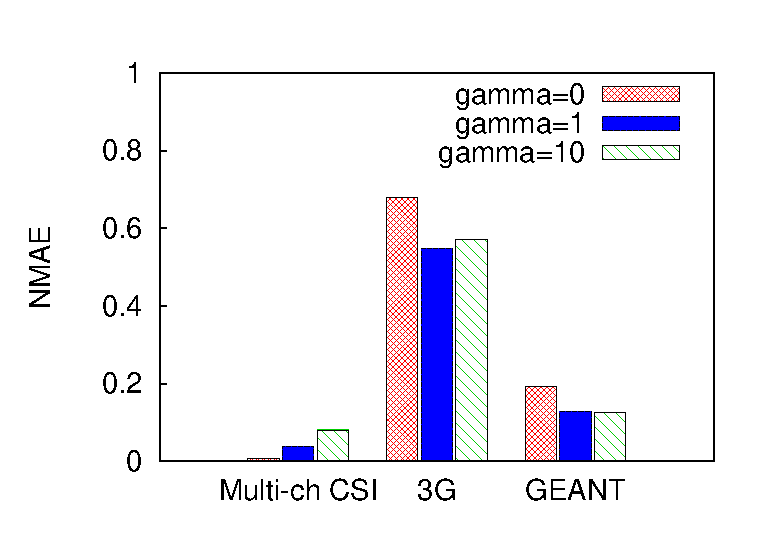
\includegraphics[width=\figurewidthB]{fig_lens3/trace.lens3.gamma.mae.eps}
  }
  \subfigure[$\gamma$ under different conditions]{
    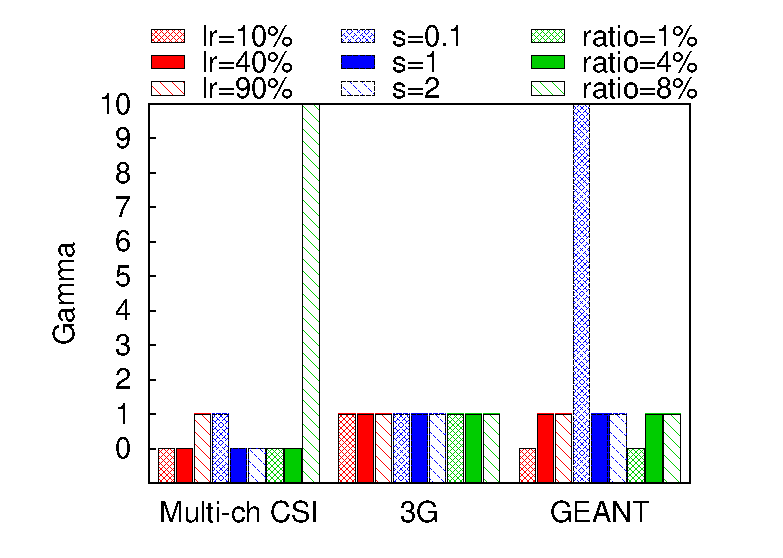
\includegraphics[width=\figurewidthB]{fig_lens3/trace.lens3.gamma.vary_param.eps}
  }
  % \caption{(a) NMAE of different $\gamma$: learned $\gamma$ is $0$ for
  %   multi-channel CSI, $1$ for 3G, and $10$ for G\'{E}ANT under no anomalies. (b) The learned $\gamma$ under loss rates = $10\%$, $40\%$, $90\%$; anomaly size $s$ = $0.1$, $1$, $2$; ratio of anomalies = $1\%$, $4\%$, $8\%$.}
  \caption{Self learned $\gamma$.}
  \label{fig:lens3-gamma}
\end{figure}


\begin{figure}[h!]
  \centering
   % \vspace{-0.1in}
  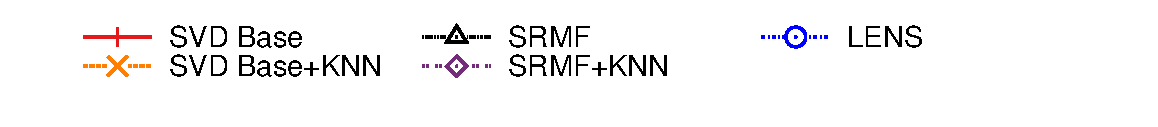
\includegraphics[width=\columnwidth]{fig/legend.eps}
  \subfigure[3G]{
    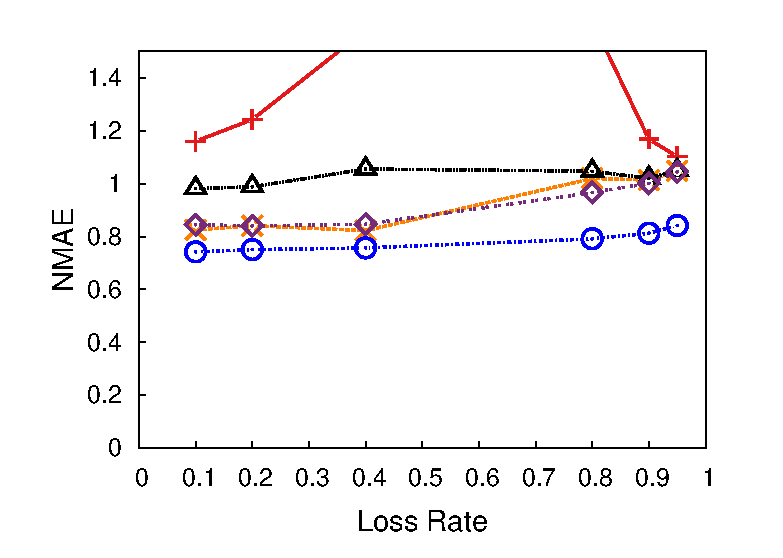
\includegraphics[width=\figurewidthI]{fig_lens3/pred.PureRandLoss.srmf_based_pred.tm_3g.cell.bs.bs3.all.bin10.txt.org.2d.elem.ind.elem1.burst1.na0.05.anom1.noise0.thresh-1.eps}
  }
  \subfigure[WiFi]{
    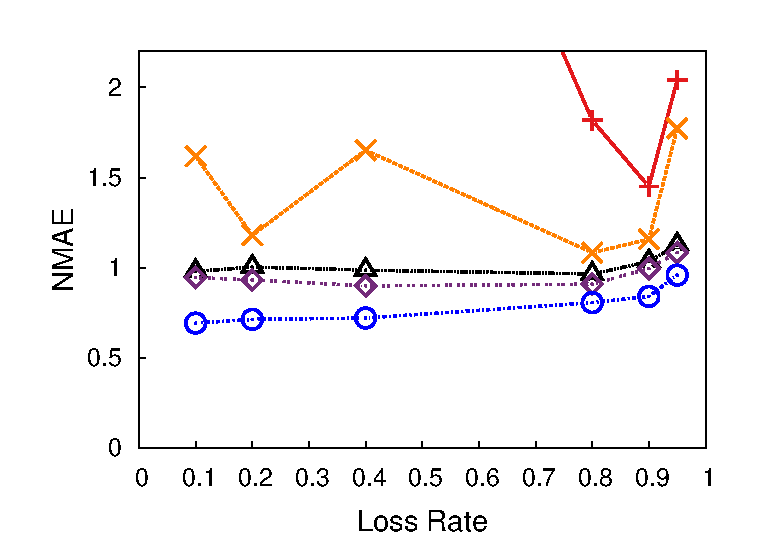
\includegraphics[width=\figurewidthI]{fig_lens3/pred.PureRandLoss.srmf_based_pred.tm_sjtu_wifi.ap_load.all.bin600.top50.txt.org.2d.elem.ind.elem1.burst1.na0.05.anom1.noise0.thresh-1.eps}
  }
  \subfigure[Abilene]{
    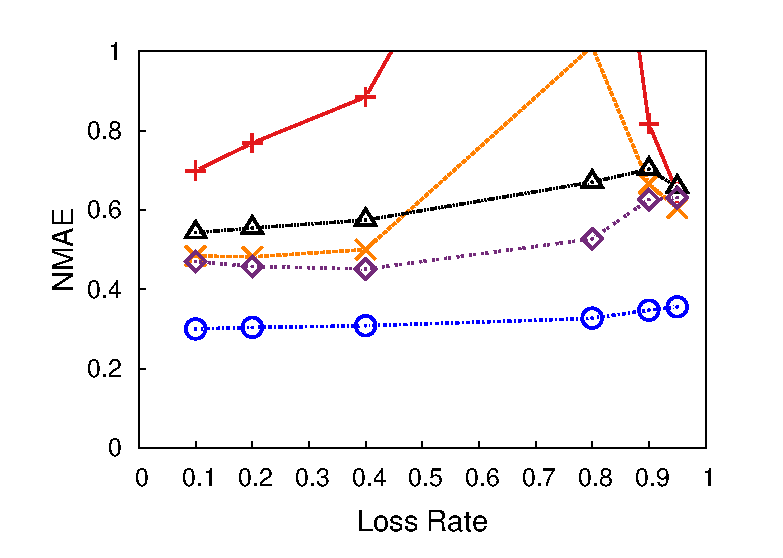
\includegraphics[width=\figurewidthI]{fig_lens3/pred.PureRandLoss.srmf_based_pred.tm_abilene.od..org.2d.elem.ind.elem1.burst1.na0.05.anom1.noise0.thresh-1.eps}
  }
  \subfigure[G\'{E}ANT]{
    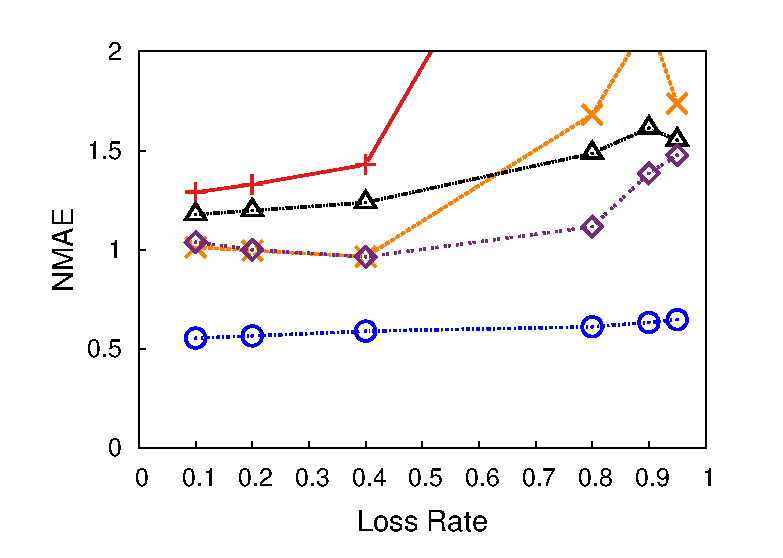
\includegraphics[width=\figurewidthI]{fig_lens3/pred.PureRandLoss.srmf_based_pred.tm_totem..org.2d.elem.ind.elem1.burst1.na0.05.anom1.noise0.thresh-1.eps}
  }
  \subfigure[1-channel CSI]{
    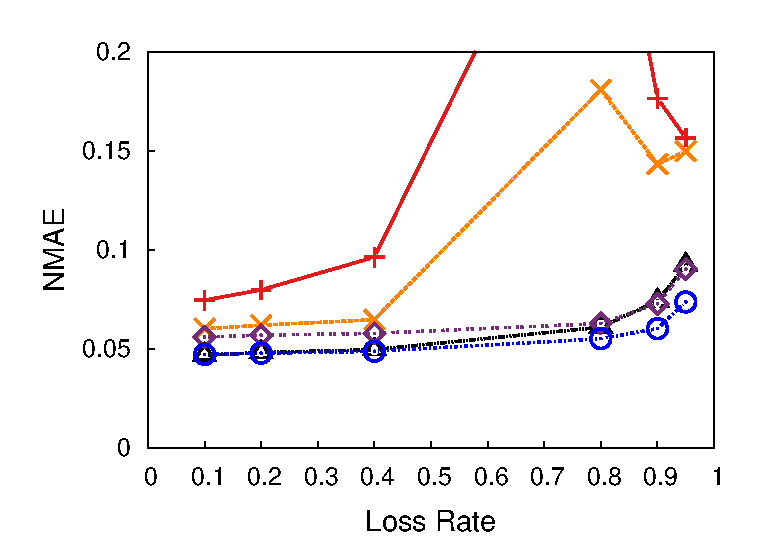
\includegraphics[width=\figurewidthI]{fig_lens3/pred.PureRandLoss.srmf_based_pred.Mob-Recv1run1.dat0_matrix.mat_dB.txt.org.2d.elem.ind.elem1.burst1.na0.05.anom1.noise0.thresh-1.eps}
  }
  \subfigure[Multi-channel CSI]{
    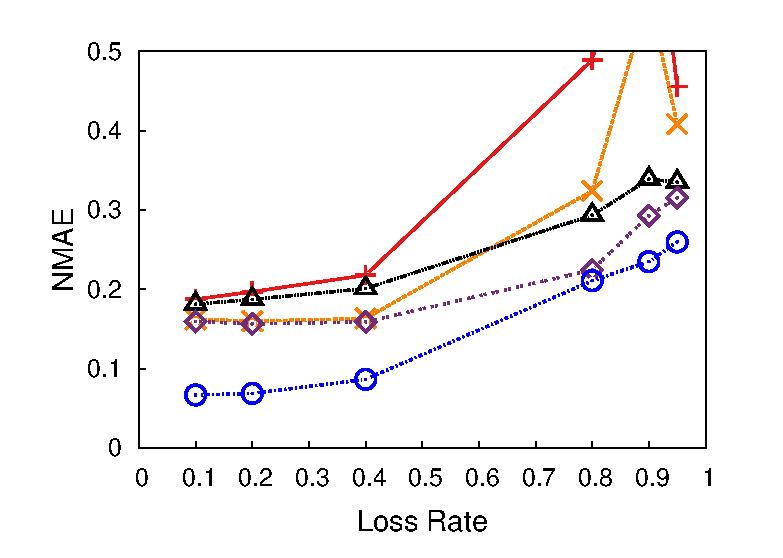
\includegraphics[width=\figurewidthI]{fig_lens3/pred.PureRandLoss.srmf_based_pred.static_trace13.ant1.mag.txt.org.2d.elem.ind.elem1.burst1.na0.05.anom1.noise0.thresh-1.eps}
  }
  \subfigure[Cister RSSI]{
    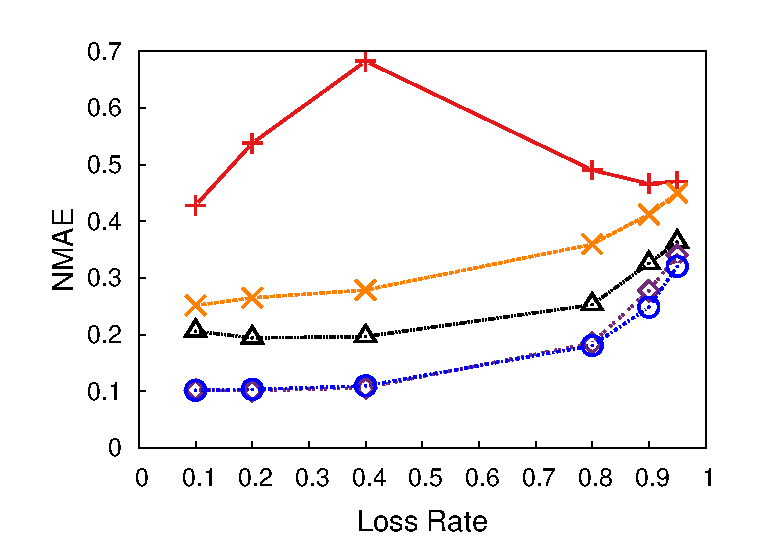
\includegraphics[width=\figurewidthI]{fig_lens3/pred.PureRandLoss.srmf_based_pred.tm_telos_rssi.txt.org.2d.elem.ind.elem1.burst1.na0.05.anom1.noise0.thresh-1.eps}
  }
  \subfigure[CU RSSI]{
    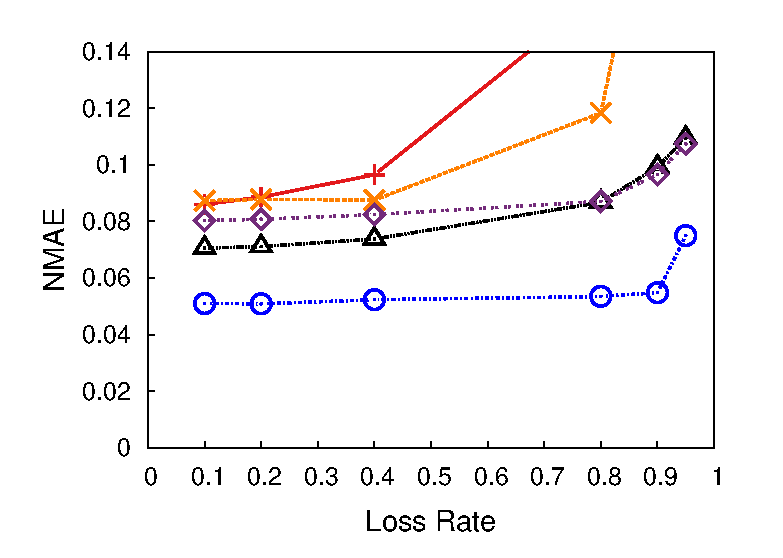
\includegraphics[width=\figurewidthI]{fig_lens3/pred.PureRandLoss.srmf_based_pred.tm_multi_loc_rssi.txt.org.2d.elem.ind.elem1.burst1.na0.05.anom1.noise0.thresh-1.eps}
  }
  \subfigure[UMich RSS]{
    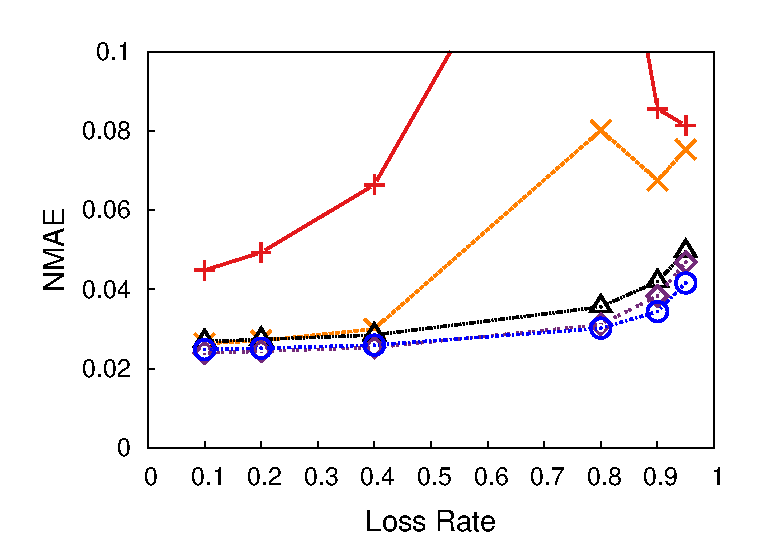
\includegraphics[width=\figurewidthI]{fig_lens3/pred.PureRandLoss.srmf_based_pred.tm_umich_rss.txt.org.2d.elem.ind.elem1.burst1.na0.05.anom1.noise0.thresh-1.eps}
  }
  \subfigure[UCSB Meshnet]{
    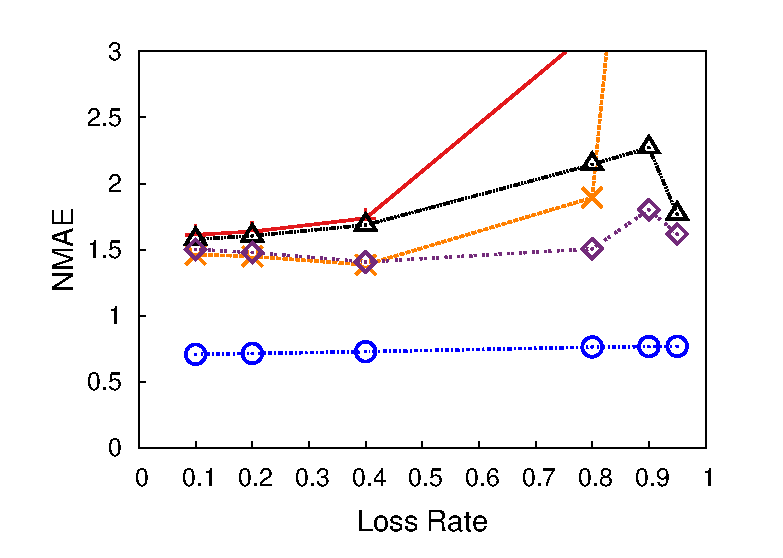
\includegraphics[width=\figurewidthI]{fig_lens3/pred.PureRandLoss.srmf_based_pred.tm_ucsb_meshnet.connected.txt.org.2d.elem.ind.elem1.burst1.na0.05.anom1.noise0.thresh-1.eps}
  }
%  \hspace{-0.1in}
%  \subfigure[Delay]{
%    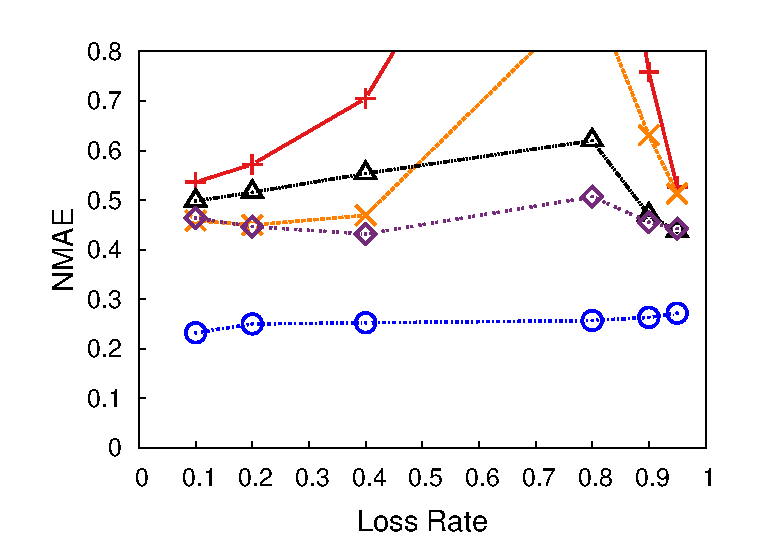
\includegraphics[width=\figurewidthQ]{fig_lens3/pred.PureRandLoss.srmf_based_pred.tm_ron1.latency..org.2d.elem.ind.elem1.burst1.na0.05.anom1.noise0.thresh-1.eps}
%  }
  % \caption{Interpolation performance under varying data loss rates
  %   under 5\% anomalies and $s=1$.}
  \caption{Interpolation performance under varying data loss rates.}
  \label{fig:pure-rand-interpolation}
\end{figure}

\begin{figure}[h!]
  \centering
  \includegraphics[width=1\columnwidth]{fig/legend.eps}
  \subfigure[3G]{
    \includegraphics[width=\figurewidthI]{fig_lens3/pred.PureRandLoss.srmf_based_pred.tm_3g.cell.bs.bs3.all.bin10.txt.org.2d.elem.ind.elem1.burst1.na0.05.anom0.noise0.thresh-1.eps}
  }
  \subfigure[WiFi]{
    \includegraphics[width=\figurewidthI]{fig_lens3/pred.PureRandLoss.srmf_based_pred.tm_sjtu_wifi.ap_load.all.bin600.top50.txt.org.2d.elem.ind.elem1.burst1.na0.05.anom0.noise0.thresh-1.eps}
  }
  \subfigure[Abilene]{
    \includegraphics[width=\figurewidthI]{fig_lens3/pred.PureRandLoss.srmf_based_pred.tm_abilene.od..org.2d.elem.ind.elem1.burst1.na0.05.anom0.noise0.thresh-1.eps}
  }
  \subfigure[G\'{E}ANT]{
    \includegraphics[width=\figurewidthI]{fig_lens3/pred.PureRandLoss.srmf_based_pred.tm_totem..org.2d.elem.ind.elem1.burst1.na0.05.anom0.noise0.thresh-1.eps}
  }
  \subfigure[1-channel CSI]{
    \includegraphics[width=\figurewidthI]{fig_lens3/pred.PureRandLoss.srmf_based_pred.Mob-Recv1run1.dat0_matrix.mat_dB.txt.org.2d.elem.ind.elem1.burst1.na0.05.anom0.noise0.thresh-1.eps}
  }
  \subfigure[Multi-channel CSI]{
    \includegraphics[width=\figurewidthI]{fig_lens3/pred.PureRandLoss.srmf_based_pred.static_trace13.ant1.mag.txt.org.2d.elem.ind.elem1.burst1.na0.05.anom0.noise0.thresh-1.eps}
  }
  \subfigure[Cister RSSI]{
    \includegraphics[width=\figurewidthI]{fig_lens3/pred.PureRandLoss.srmf_based_pred.tm_telos_rssi.txt.org.2d.elem.ind.elem1.burst1.na0.05.anom0.noise0.thresh-1.eps}
  }
  \subfigure[CU RSSI]{
    \includegraphics[width=\figurewidthI]{fig_lens3/pred.PureRandLoss.srmf_based_pred.tm_multi_loc_rssi.txt.org.2d.elem.ind.elem1.burst1.na0.05.anom0.noise0.thresh-1.eps}
  }
  \subfigure[UMich RSS]{
    \includegraphics[width=\figurewidthI]{fig_lens3/pred.PureRandLoss.srmf_based_pred.tm_umich_rss.txt.org.2d.elem.ind.elem1.burst1.na0.05.anom0.noise0.thresh-1.eps}
  }
  \subfigure[UCSB Meshnet]{
    \includegraphics[width=\figurewidthI]{fig_lens3/pred.PureRandLoss.srmf_based_pred.tm_ucsb_meshnet.connected.txt.org.2d.elem.ind.elem1.burst1.na0.05.anom0.noise0.thresh-1.eps}
  }
%  \hspace{-0.1in}
%  \subfigure[Delay]{
%    \includegraphics[width=\figurewidthQ]{fig_lens3/pred.PureRandLoss.srmf_based_pred.tm_ron1.latency..org.2d.elem.ind.elem1.burst1.na0.05.anom0.noise0.thresh-1.eps}
%  }
  \caption{Varying data loss rates and no anomaly}
  \label{fig:pure-rand-no-anomaly}
\end{figure}

% \begin{figure}[h!]
%   \centering
%   %  \vspace{-0.6in}
%   \includegraphics[width=1\columnwidth]{fig/legend.eps}
%   \subfigure[CSI]{
%     % \includegraphics[width=\figurewidthQ]{fig/pred.PureRandLoss.srmf_based_pred.Mob-Recv1run1.dat0_matrix.mat_dB.txt.1000.90.1.1000.r32.period1.org.2d.elem.ind.elem1.burst1.na0.05.anom0.4.noise0.thresh0.eps}
%     \includegraphics[width=\figurewidthQ]{fig/pred.PureRandLoss.srmf_based_pred.Mob-Recv1run1.dat0_matrix.mat_dB.txt.1000.90.1.1000.r32.period1.org.2d.elem.ind.elem1.burst1.na0.05.anom3.noise0.thresh-1.eps}
%   }
%   \hspace{-0.1in}
%   \subfigure[Cister RSSI]{
%     % \includegraphics[width=\figurewidthQ]{fig/pred.PureRandLoss.srmf_based_pred.tm_telos_rssi.txt.1000.16.1.1000.r8.period1.org.2d.elem.ind.elem1.burst1.na0.05.anom0.4.noise0.thresh0.eps}
%     \includegraphics[width=\figurewidthQ]{fig/pred.PureRandLoss.srmf_based_pred.tm_telos_rssi.txt.500.16.1.500.r4.period1.org.2d.elem.ind.elem1.burst1.na0.05.anom3.noise0.thresh-1.eps}
%   }
%   \hspace{-0.1in}
%   \subfigure[CU RSSI]{
%     % \includegraphics[width=\figurewidthQ]{fig/pred.PureRandLoss.srmf_based_pred.tm_multi_loc_rssi.txt.500.895.1.500.r32.period1.org.2d.elem.ind.elem1.burst1.na0.05.anom0.4.noise0.thresh0.eps}
%     \includegraphics[width=\figurewidthQ]{fig/pred.PureRandLoss.srmf_based_pred.tm_multi_loc_rssi.txt.500.895.1.500.r32.period1.org.2d.elem.ind.elem1.burst1.na0.05.anom3.noise0.thresh-1.eps}
%   }
%   %\hspace{-0.1in}
%   %\subfigure[Delay]{
%   %  \includegraphics[width=\figurewidthQ]{fig/pred.PureRandLoss.srmf_based_pred.tm_ron1.latency..494.12.12.494.r8.period1.org.2d.elem.ind.elem1.burst1.na0.05.anom0.4.noise0.thresh0.eps}
%   %}
%   \vspace{-0.1in}
%   \caption{Interpolation performance of CSI and RSS matrices under
%     varying data loss rates, 5\% anomalies, and $k=1$.}
%   \vspace{-0.1in}
%   \label{fig:pure-rand-interpolation-rssi}
% \end{figure}


\subsection{Performance Results}
\label{ssec:eval-results}

\para{Self learned $\gamma$:} LENS supports many types of 
domain knowledge as described in Sec.~\ref{ssec:lens}. Our evaluation only
considered temporal stability for simplicity and $\gamma$ reflects its importance. 
To illustrate the benefit of self learning, Figure~\ref{fig:lens3-gamma} (a) shows the performance under
different $\gamma$ values and different traces. Figure~\ref{fig:lens3-gamma} (b) shows 
the best $\gamma$ under different traces, loss rates, anomaly sizes, and ratio of anomalies. 
There does not exist a single $\gamma$ that
works well for all traces or conditions. Self tuning allows us to
automatically select the best $\gamma$ for these traces and achieves
low NMAE in all cases. 


\para{Varying dropping rates:} We first compare different schemes in
terms of interpolation accuracy measured using NMAE.
% Second, LENS+SRMF+KNN performs similarly to LENS and LENS+KNN
% when loss is 80\% or lower, and out-performs LENS and LENS+KNN when
% loss rate is 90\% or higher. The latter is because when data loss rate
% is very high, the system is severely under-constrained and the need to
% estimate additional unknowns in the general formulation in LENS makes
% the system further under-constrained and incurs higher
% error. LENS+SRMF+KNN leverages the anomaly detection from LENS while
% keeping the number of unknowns small, thereby achieving better performance. 
% Next we evaluate the performance under anomalies. We inject anomalies
% to a portion of the entries in the original matrix. The anomalies
% follow a uniform distribution
Figure~\ref{fig:pure-rand-interpolation} shows the interpolation error
% as we randomly inject anomalies to 5\% elements.
% We set the anomaly size in Abilene, G\'{E}ANT, 3G, WiFi, and RON matrices 
%  with an uniformly distributed number between $[0.2, 0.4]$, and CSI, Cister RSSI,
%  and CU RSSI matrices with an uniformly distributed number between $[std, 2std]$.
%  In the following paper, this anomaly size is used in default if not mentioned 
%  specifically.
% First, we observe that the benefit of LENS and the
as we randomly inject anomalies to 5\% elements with $s=1$. For clarity of the graphs, we cap the y-axis so
that we can focus on the most interesting parts of the graphs. 
% Some points on certain curves are outside the range and not shown. 
% First,
We observe that % the benefit of LENS
% and the combined scheme
% increases under anomalies, as we would
% expect.
% LENS+SRMF+KNN $<$ LENS+KNN, LENS
LENS consistently out-performs the other schemes. In terms of NMAE,
LENS $<$ SRMF + KNN $<$
 SRMF $<$ SVD Base + KNN $<$ SVD Base.
% Second, the benefit of LENS
%  varies across the traces. For example, in XXX, XXX, XXX,
 LENS reduces NMAE by 35.5\% over SRMF, 27.8\% over SRMF+KNN, 59.8\%
 over SVD Base, and 44.9\% over SVD Base + KNN on average. Moreover,
 the error is low for high-rank matrices. For example, the highest
 rank matrices in our datasets are 1-channel CSI, CU RSSI, Abilene,
 WiFi, 3G, and Cister RSSI matrices. Their corresponding NMAE are
 0.05, 0.05, 0.3, 0.69, 0.74, 0.1, respectively. Most of them have low
 errors except WiFi and 3G. % The reason for WiFi and 3G to have high
% errors is that XXX.
The error does not monotonically increase with
the loss rate because an increasing loss rate reduces the number of
anomalies, which may help reduce the error. 

% Second, it is interesting to see that KNN
% sometimes degrades the
% performance of SRMF and SVD under anomalies. This is because nearby
% anomalies can 
% propagate its value and contaminate estimation of the normal
% entries. In contrast, LENS does not have contamination problem when
% using temporal and spatial locality since these locality are imposed
% on $X$ after removing anomalies $Y$ estimated by LENS.

Figure~\ref{fig:pure-rand-no-anomaly} summarizes the results under
varying data loss rates and no anomaly. In most traces, LENS performs
comparably to SRMF+KNN, the best known algorithm under no anomaly.
In UCSB Meshnet, LENS already out-performs SRMF+KNN even
without injecting additional anomalies. This is likely because the
trace has more anomalies before our anomaly injection. In UCSB Meshnet trace,
3.2\% of EWMA prediction errors are larger than 5 times standard deviation 
from mean, whereas the corresponding numbers in other traces are
1.2\%-2.4\%. 3G trace has the second largest number of EWMA prediction error 
where we can also see LENS shows 7.7\% improvement over SRMF+KNN.
% We make several
% observations. First, without anomalies, LENS already out-performs 
% all the existing schemes especially under high loss rates. This is
% because XXX. Second,  
% SRMF+KNN performs the second best. Both LENS and SRMF out-perform SVD
% Base and SVD Base + KNN.

%LENS+SRMF+KNN consistently works well because we
%apply KNN to the matrix after removing the anomalies estimated by
%LENS, thereby avoiding the contamination problem. 

\comment{
Figure~\ref{fig:pure-rand-interpolation-rssi} compares interpolation
error when we inject anomalies to RSSI matrices. LENS
consistently performs the best. It out-performs SRMF and SRMF+KNN
by XXX\% and XXX\%, respectively, and out-performs SVD base and SVD base +
KNN by XXX\% and XXX\%, respectively.
}

% Therefore, we can see that SVD Base+KNN under-performs SVD Base and
% SRMF+KNN under-performs SRMF in many cases. LENS+KNN, on the other
% hand, still benefits LENS because LENS decomposes the matrix into
% different components and we apply KNN to the matrix after
% subtracting the anomalies. 


\begin{figure}[h!]
  \centering
  \includegraphics[width=1\columnwidth]{fig/legend.eps}
  \subfigure[3G]{
    \includegraphics[width=\figurewidthI]{fig_lens3/pred.AnomalySize.srmf_based_pred.tm_3g.cell.bs.bs3.all.bin10.txt.144.472.1.144.r32.period1.org.2d.elem.ind.elem1.lr0.5.burst1.na0.05.noise0.thresh-1.eps}
  }
  \subfigure[WiFi]{
    \includegraphics[width=\figurewidthI]{fig_lens3/pred.AnomalySize.srmf_based_pred.tm_sjtu_wifi.ap_load.all.bin600.top50.txt.100.50.1.100.r8.period1.org.2d.elem.ind.elem1.lr0.5.burst1.na0.05.noise0.thresh-1.eps}
  }
  \subfigure[Abilene]{
    \includegraphics[width=\figurewidthI]{fig_lens3/pred.AnomalySize.srmf_based_pred.tm_abilene.od..1008.11.11.1008.r20.period1.org.2d.elem.ind.elem1.lr0.5.burst1.na0.05.noise0.thresh-1.eps}
  }
  \subfigure[G\'{E}ANT]{
    \includegraphics[width=\figurewidthI]{fig_lens3/pred.AnomalySize.srmf_based_pred.tm_totem..672.23.23.672.r25.period1.org.2d.elem.ind.elem1.lr0.5.burst1.na0.05.noise0.thresh-1.eps}
  }
  \subfigure[1-channel CSI]{
   \includegraphics[width=\figurewidthI]{fig_lens3/pred.AnomalySize.srmf_based_pred.Mob-Recv1run1.dat0_matrix.mat_dB.txt.1000.90.1.1000.r16.period1.org.2d.elem.ind.elem1.lr0.5.burst1.na0.05.noise0.thresh-1.eps}
  }
  \subfigure[Multi-channel CSI]{
    \includegraphics[width=\figurewidthI]{fig_lens3/pred.AnomalySize.srmf_based_pred.static_trace13.ant1.mag.txt.500.270.1.500.r16.period1.org.2d.elem.ind.elem1.lr0.5.burst1.na0.05.noise0.thresh-1.eps}
  }
  \subfigure[Cister RSSI]{
   \includegraphics[width=\figurewidthI]{fig_lens3/pred.AnomalySize.srmf_based_pred.tm_telos_rssi.txt.500.16.1.500.r8.period1.org.2d.elem.ind.elem1.lr0.5.burst1.na0.05.noise0.thresh-1.eps}
  }
  \subfigure[CU RSSI]{
   \includegraphics[width=\figurewidthI]{fig_lens3/pred.AnomalySize.srmf_based_pred.tm_multi_loc_rssi.txt.500.895.1.500.r16.period1.org.2d.elem.ind.elem1.lr0.5.burst1.na0.05.noise0.thresh-1.eps}
  }
  \subfigure[UMich RSS]{
    \includegraphics[width=\figurewidthI]{fig_lens3/pred.AnomalySize.srmf_based_pred.tm_umich_rss.txt.1000.182.1.1000.r32.period1.org.2d.elem.ind.elem1.lr0.5.burst1.na0.05.noise0.thresh-1.eps}
  }
  \subfigure[UCSB Meshnet]{
    \includegraphics[width=\figurewidthI]{fig_lens3/pred.AnomalySize.srmf_based_pred.tm_ucsb_meshnet.connected.txt.1000.425.1.1000.r16.period1.org.2d.elem.ind.elem1.lr0.5.burst1.na0.05.noise0.thresh-1.eps}
  }
%  \hspace{-0.1in}
%  \subfigure[Delay]{
%    \includegraphics[width=\figurewidthQ]{fig_lens3/pred.AnomalySize.srmf_based_pred.tm_ron1.latency..494.12.12.494.r16.period1.org.2d.elem.ind.elem1.lr0.5.burst1.na0.05.noise0.thresh-1.eps}
%  }
  \caption{Impact of anomaly sizes.}
  \label{fig:anomaly-size-interpolation}
\end{figure}

\para{Varying anomaly sizes:}
Figure~\ref{fig:anomaly-size-interpolation} shows the interpolation
performance as we vary the anomaly size $s$. LENS 
significantly out-performs all the other schemes. Its benefit
increases with the anomaly size. For example, when $s=1$,
the NMAE of LENS is 33.7\% lower than SRMF,
20.2\% lower than SRMF+KNN, 61.8\% lower than SVD Base, and 34.8\% lower than
SVD Base+KNN. The corresponding numbers under $s=2$ are 44.9\%,
31.9\%, 69.8\%, and 45.8\%, respectively. Moreover, as we would expect, NMAE of
all schemes tends to increase with the anomaly size in all traces,
though the NMAE of LENS increases more slowly than the
other schemes, since LENS explicitly separates anomalies before data
interpolation. 
% Comparing different LENS variants,
% LENS+SRMF+KNN slightly out-performs LENS and LENS+KNN in 3G and WiFi
% traces, and performs similarly in the other traces.
These results highlight the importance of anomaly detection in interpolation.

% \begin{figure}[h!]
%   \centering
%  % \vspace{-0.6in}
%   \includegraphics[width=1\columnwidth]{fig/legend.eps}
%   \subfigure[CSI]{
%     % \includegraphics[width=\figurewidthQ]{fig/pred.AnomalySize.srmf_based_pred.Mob-Recv1run1.dat0_matrix.mat_dB.txt.1000.90.1.1000.r32.period1.org.2d.elem.ind.elem1.lr0.5.burst1.na0.05.noise0.thresh0.eps}
%     \includegraphics[width=\figurewidthQ]{fig/pred.AnomalySize.srmf_based_pred.Mob-Recv1run1.dat0_matrix.mat_dB.txt.1000.90.1.1000.r32.period1.org.2d.elem.ind.elem1.lr0.5.burst1.na0.05.noise0.thresh-1.eps}
%   }
%   \hspace{-0.1in}
%   \subfigure[Cister RSSI]{
%     % \includegraphics[width=\figurewidthQ]{fig/pred.AnomalySize.srmf_based_pred.tm_telos_rssi.txt.1000.16.1.1000.r8.period1.org.2d.elem.ind.elem1.lr0.5.burst1.na0.05.noise0.thresh0.eps}
%     \includegraphics[width=\figurewidthQ]{fig/pred.AnomalySize.srmf_based_pred.tm_telos_rssi.txt.1000.16.1.1000.r8.period1.org.2d.elem.ind.elem1.lr0.5.burst1.na0.05.noise0.thresh-1.eps}
%   }
%   \hspace{-0.1in}
%   \subfigure[CU RSSI]{
%     % \includegraphics[width=\figurewidthQ]{fig/pred.AnomalySize.srmf_based_pred.tm_multi_loc_rssi.txt.500.895.1.500.r32.period1.org.2d.elem.ind.elem1.lr0.5.burst1.na0.05.noise0.thresh0.eps}
%     \includegraphics[width=\figurewidthQ]{fig/pred.AnomalySize.srmf_based_pred.tm_multi_loc_rssi.txt.500.895.1.500.r32.period1.org.2d.elem.ind.elem1.lr0.5.burst1.na0.05.noise0.thresh-1.eps}
%   }
% %  \hspace{-0.1in}
% %  \subfigure[Delay]{
% %    \includegraphics[width=\figurewidthQ]{fig/pred.AnomalySize.srmf_based_pred.tm_ron1.latency..494.12.12.494.r8.period1.org.2d.elem.ind.elem1.lr0.5.burst1.na0.05.noise0.thresh0.eps}
% %  }
%   \vspace{-0.1in}
%   \caption{Impact of anomaly sizes on CSI and RSS traces when ratio of anomalies = 5\% and loss rate = 50\%.}
%   \vspace{-0.1in}
%   \label{fig:anomaly-size-interpolation-rss}
% \end{figure}

% Figure~\ref{fig:anomaly-size-interpolation-rss} shows the impact of
% anomaly sizes on RSS traces as we vary $k$. As in traffic and delay
% matrices, the benefit of LENS increases with anomaly sizes. For
% example, when $k=1$, the benefit over SRMF+KNN, SRMF, SVD+KNN, and SVD
% are 21.3\%, 33.7\%, 45.5\%, and 75.7\%, respectively. The
% corresponding numbers increase to 34.6\%, 33.5\%, 53.4\%, and 77.6\%, respectively, when $k=4$.


\begin{figure}[h!]
  \centering
  \includegraphics[width=1\columnwidth]{fig/legend.eps}
  \subfigure[3G]{
    \includegraphics[width=\figurewidthI]{fig_lens3/pred.NumAnomaly.srmf_based_pred.tm_3g.cell.bs.bs3.all.bin10.txt.144.472.1.144.r32.period1.org.2d.elem.ind.elem1.lr0.5.burst1.anom1.noise0.thresh-1.eps}
  }
  \subfigure[WiFi]{
    \includegraphics[width=\figurewidthI]{fig_lens3/pred.NumAnomaly.srmf_based_pred.tm_sjtu_wifi.ap_load.all.bin600.top50.txt.100.50.1.100.r8.period1.org.2d.elem.ind.elem1.lr0.5.burst1.anom1.noise0.thresh-1.eps}
  }
  \subfigure[Abilene]{
    \includegraphics[width=\figurewidthI]{fig_lens3/pred.NumAnomaly.srmf_based_pred.tm_abilene.od..1008.11.11.1008.r20.period1.org.2d.elem.ind.elem1.lr0.5.burst1.anom1.noise0.thresh-1.eps}
  }
  \subfigure[G\'{E}ANT]{
    \includegraphics[width=\figurewidthI]{fig_lens3/pred.NumAnomaly.srmf_based_pred.tm_totem..672.23.23.672.r25.period1.org.2d.elem.ind.elem1.lr0.5.burst1.anom1.noise0.thresh-1.eps}
  }
  \subfigure[1-channel CSI]{
   \includegraphics[width=\figurewidthI]{fig_lens3/pred.NumAnomaly.srmf_based_pred.Mob-Recv1run1.dat0_matrix.mat_dB.txt.1000.90.1.1000.r16.period1.org.2d.elem.ind.elem1.lr0.5.burst1.anom1.noise0.thresh-1.eps}
  }
  \subfigure[Multi-channel CSI]{
    \includegraphics[width=\figurewidthI]{fig_lens3/pred.NumAnomaly.srmf_based_pred.static_trace13.ant1.mag.txt.500.270.1.500.r16.period1.org.2d.elem.ind.elem1.lr0.5.burst1.anom1.noise0.thresh-1.eps}
  }
  \subfigure[Cister RSSI]{
   \includegraphics[width=\figurewidthI]{fig_lens3/pred.NumAnomaly.srmf_based_pred.tm_telos_rssi.txt.500.16.1.500.r8.period1.org.2d.elem.ind.elem1.lr0.5.burst1.anom1.noise0.thresh-1.eps}
  }
  \subfigure[CU RSSI]{
   \includegraphics[width=\figurewidthI]{fig_lens3/pred.NumAnomaly.srmf_based_pred.tm_multi_loc_rssi.txt.500.895.1.500.r16.period1.org.2d.elem.ind.elem1.lr0.5.burst1.anom1.noise0.thresh-1.eps}
  }
  \subfigure[UMich RSS]{
    \includegraphics[width=\figurewidthI]{fig_lens3/pred.NumAnomaly.srmf_based_pred.tm_umich_rss.txt.1000.182.1.1000.r32.period1.org.2d.elem.ind.elem1.lr0.5.burst1.anom1.noise0.thresh-1.eps}
  }
  \subfigure[UCSB Meshnet]{
    \includegraphics[width=\figurewidthI]{fig_lens3/pred.NumAnomaly.srmf_based_pred.tm_ucsb_meshnet.connected.txt.1000.425.1.1000.r16.period1.org.2d.elem.ind.elem1.lr0.5.burst1.anom1.noise0.thresh-1.eps}
  }
  % \caption{Impact of number of anomalies when the loss rate = 50\% and
  %   $s=1$.}
  \caption{Impact of number of anomalies.}
  \label{fig:anomaly-number-interpolation}
\end{figure}

\para{Varying the number of anomalies:}
Figure~\ref{fig:anomaly-number-interpolation} shows the interpolation
performance as we vary the number of anomalies. As before, LENS
out-performs SRMF and SVD based schemes. 
% Its benefits increase with the number of anomalies. 
The improvement ranges between
25.3-59.7\% with 8\% anomalies and 30.1-54.5\% with 16\% anomalies. In
addition, the NMAE increases with the number of anomalies.
% [XXX: double check] Some traces,
% such as Abilene and G\'{E}ANT see sharper increases in NMAE
% while other traces experience more graduate increases.
Among different
schemes, the rate of increase is slowest in LENS due to its
explicit anomaly detection and removal.
%% LENS becomes less beneficial with 10\% anomalies because of the exceptions in CU RSSI

% \begin{figure}[h!]
%   \centering
%   \includegraphics[width=1\columnwidth]{fig/legend.eps}
%   \subfigure[CSI]{
%     % \includegraphics[width=\figurewidthQ]{fig/pred.NumAnomaly.srmf_based_pred.Mob-Recv1run1.dat0_matrix.mat_dB.txt.1000.90.1.1000.r32.period1.org.2d.elem.ind.elem1.lr0.5.burst1.anom0.4.noise0.thresh0.eps}
%     \includegraphics[width=\figurewidthQ]{fig/pred.NumAnomaly.srmf_based_pred.Mob-Recv1run1.dat0_matrix.mat_dB.txt.1000.90.1.1000.r32.period1.org.2d.elem.ind.elem1.lr0.5.burst1.anom3.noise0.thresh-1.eps}
%   }
%   \hspace{-0.1in}
%   \subfigure[Cister RSSI]{
%     % \includegraphics[width=\figurewidthQ]{fig/pred.NumAnomaly.srmf_based_pred.tm_telos_rssi.txt.1000.16.1.1000.r8.period1.org.2d.elem.ind.elem1.lr0.5.burst1.anom0.4.noise0.thresh0.eps}
%     \includegraphics[width=\figurewidthQ]{fig/pred.NumAnomaly.srmf_based_pred.tm_telos_rssi.txt.1000.16.1.1000.r8.period1.org.2d.elem.ind.elem1.lr0.5.burst1.anom3.noise0.thresh-1.eps}
%   }
%   \hspace{-0.1in}
%   \subfigure[CU RSSI]{
%     % \includegraphics[width=\figurewidthQ]{fig/pred.NumAnomaly.srmf_based_pred.tm_multi_loc_rssi.txt.500.895.1.500.r32.period1.org.2d.elem.ind.elem1.lr0.5.burst1.anom0.4.noise0.thresh0.eps}
%     \includegraphics[width=\figurewidthQ]{fig/pred.NumAnomaly.srmf_based_pred.tm_multi_loc_rssi.txt.500.895.1.500.r32.period1.org.2d.elem.ind.elem1.lr0.5.burst1.anom3.noise0.thresh-1.eps}
%   }
%   \caption{Impact of number of anomalies on CSI and RSS traces when the loss rate = 50\%.}
%   \vspace{-0.1in}
%   \label{fig:anomaly-number-interpolation-rss}
% \end{figure}

%Figure~\ref{fig:anomaly-number-interpolation-rss} shows the
%interpolation accuracy of CSI and RSS matrices. We observe similar
%trend as in traffic and delay matrices.

\para{Varying noise sizes:}
Figure~\ref{fig:noise-size-interpolation} shows the interpolation
performance as we vary the noise sizes. We inject noise to all the 
elements in the original matrices. The size of the noise follows 
normal distribution with mean $0$ and standard deviation $\sigma$
where $\sigma$ is varied from $1\%$ to $64\%$ of the maximal value
in the matrix. As before, LENS out-performs the other schemes. 

\begin{figure}[h!]
  \centering
  \includegraphics[width=1\columnwidth]{fig/legend.eps}
  \subfigure[3G]{
    \includegraphics[width=\figurewidthI]{fig_lens3/pred.NoiseSize.srmf_based_pred.tm_3g.cell.bs.bs3.all.bin10.txt.144.472.1.144.r32.period1.org.2d.elem.ind.elem1.lr0.5.burst1.na0.anom0.thresh-1.eps}
  }
  \subfigure[WiFi]{
    \includegraphics[width=\figurewidthI]{fig_lens3/pred.NoiseSize.srmf_based_pred.tm_sjtu_wifi.ap_load.all.bin600.top50.txt.100.50.1.100.r8.period1.org.2d.elem.ind.elem1.lr0.5.burst1.na0.anom0.thresh-1.eps}
  }
  \subfigure[Abilene]{
    \includegraphics[width=\figurewidthI]{fig_lens3/pred.NoiseSize.srmf_based_pred.tm_abilene.od..1008.11.11.1008.r20.period1.org.2d.elem.ind.elem1.lr0.5.burst1.na0.anom0.thresh-1.eps}
  }
  \subfigure[G\'{E}ANT]{
    \includegraphics[width=\figurewidthI]{fig_lens3/pred.NoiseSize.srmf_based_pred.tm_totem..672.23.23.672.r25.period1.org.2d.elem.ind.elem1.lr0.5.burst1.na0.anom0.thresh-1.eps}
  }
  \subfigure[1-channel CSI]{
   \includegraphics[width=\figurewidthI]{fig_lens3/pred.NoiseSize.srmf_based_pred.Mob-Recv1run1.dat0_matrix.mat_dB.txt.1000.90.1.1000.r16.period1.org.2d.elem.ind.elem1.lr0.5.burst1.na0.anom0.thresh-1.eps}
  }
  \subfigure[Multi-channel CSI]{
    \includegraphics[width=\figurewidthI]{fig_lens3/pred.NoiseSize.srmf_based_pred.static_trace13.ant1.mag.txt.500.270.1.500.r16.period1.org.2d.elem.ind.elem1.lr0.5.burst1.na0.anom0.thresh-1.eps}
  }
  \subfigure[Cister RSSI]{
   \includegraphics[width=\figurewidthI]{fig_lens3/pred.NoiseSize.srmf_based_pred.tm_telos_rssi.txt.500.16.1.500.r8.period1.org.2d.elem.ind.elem1.lr0.5.burst1.na0.anom0.thresh-1.eps}
  }
  \subfigure[CU RSSI]{
   \includegraphics[width=\figurewidthI]{fig_lens3/pred.NoiseSize.srmf_based_pred.tm_multi_loc_rssi.txt.500.895.1.500.r16.period1.org.2d.elem.ind.elem1.lr0.5.burst1.na0.anom0.thresh-1.eps}
  }
  \subfigure[UMich RSS]{
    \includegraphics[width=\figurewidthI]{fig_lens3/pred.NoiseSize.srmf_based_pred.tm_umich_rss.txt.1000.182.1.1000.r32.period1.org.2d.elem.ind.elem1.lr0.5.burst1.na0.anom0.thresh-1.eps}
  }
  \subfigure[UCSB Meshnet]{
    \includegraphics[width=\figurewidthI]{fig_lens3/pred.NoiseSize.srmf_based_pred.tm_ucsb_meshnet.connected.txt.1000.425.1.1000.r16.period1.org.2d.elem.ind.elem1.lr0.5.burst1.na0.anom0.thresh-1.eps}
  }
%  \hspace{-0.1in}
%  \subfigure[Delay]{
%    \includegraphics[width=\figurewidthQ]{fig_lens3/pred.NoiseSize.srmf_based_pred.tm_ron1.latency..494.12.12.494.r16.period1.org.2d.elem.ind.elem1.lr0.5.burst1.na0.anom0.thresh-1.eps}
%  }
  \caption{Impact of noise sizes.}
  \label{fig:noise-size-interpolation}
\end{figure}


% \para{Performance over time:}

% Figure~\ref{fig:over-time-interpolation} shows the interpolation
% performance over time. As before, LENS constantly
% out-performs SRMF and SVD based schemes. 

% \begin{figure}[h!]
%   \centering
%   %\vspace{-0.6in}
%   \includegraphics[width=1\columnwidth]{fig/legend.eps}
%   \subfigure[3G]{
%     \includegraphics[width=\figurewidthQ]{fig_lens3/pred.MatLen.srmf_based_pred.tm_3g.cell.bs.bs3.all.bin10.txt.472.1.r32.period1.org.2d.elem.ind.elem1.lr0.5.burst1.na0.05.anom1.noise0.thresh-1.eps}
%   }
%   \hspace{-0.1in}
%   \subfigure[WiFi]{
%     \includegraphics[width=\figurewidthQ]{fig_lens3/pred.MatLen.srmf_based_pred.tm_sjtu_wifi.ap_load.all.bin600.top50.txt.50.1.r8.period1.org.2d.elem.ind.elem1.lr0.5.burst1.na0.05.anom1.noise0.thresh-1.eps}
%   }
%  \hspace{-0.1in}
%  \subfigure[Abilene]{
%     \includegraphics[width=\figurewidthQ]{fig_lens3/pred.MatLen.srmf_based_pred.tm_abilene.od..11.11.r20.period1.org.2d.elem.ind.elem1.lr0.5.burst1.na0.05.anom1.noise0.thresh-1.eps}
%   }
%   \hspace{-0.1in}
%   \subfigure[G\'{E}ANT]{
%     \includegraphics[width=\figurewidthQ]{fig_lens3/pred.MatLen.srmf_based_pred.tm_totem..23.23.r25.period1.org.2d.elem.ind.elem1.lr0.5.burst1.na0.05.anom1.noise0.thresh-1.eps}
%   }
%   \hspace{-0.1in}
%   \subfigure[1-channel CSI]{
%    \includegraphics[width=\figurewidthQ]{fig_lens3/pred.MatLen.srmf_based_pred.Mob-Recv1run1.dat0_matrix.mat_dB.txt.90.1.r16.period1.org.2d.elem.ind.elem1.lr0.5.burst1.na0.05.anom1.noise0.thresh-1.eps}
%   }
%   \hspace{-0.1in}
%   \subfigure[Multi-channel CSI]{
%     \includegraphics[width=\figurewidthQ]{fig_lens3/pred.MatLen.srmf_based_pred.static_trace13.ant1.mag.txt.270.1.r16.period1.org.2d.elem.ind.elem1.lr0.5.burst1.na0.05.anom1.noise0.thresh-1.eps}
%   }
%   \hspace{-0.1in}
%   \subfigure[Cister RSSI]{
%    \includegraphics[width=\figurewidthQ]{fig_lens3/pred.MatLen.srmf_based_pred.tm_telos_rssi.txt.16.1.r8.period1.org.2d.elem.ind.elem1.lr0.5.burst1.na0.05.anom1.noise0.thresh-1.eps}
%   }
%   \hspace{-0.1in}
%   \subfigure[CU RSSI]{
%    \includegraphics[width=\figurewidthQ]{fig_lens3/pred.MatLen.srmf_based_pred.tm_multi_loc_rssi.txt.895.1.r16.period1.org.2d.elem.ind.elem1.lr0.5.burst1.na0.05.anom1.noise0.thresh-1.eps}
%   }
%   \hspace{-0.1in}
%   \subfigure[UMich RSS]{
%     \includegraphics[width=\figurewidthQ]{fig_lens3/pred.MatLen.srmf_based_pred.tm_umich_rss.txt.182.1.r32.period1.org.2d.elem.ind.elem1.lr0.5.burst1.na0.05.anom1.noise0.thresh-1.eps}
%   }
%   \hspace{-0.1in}
%   \subfigure[UCSB Meshnet]{
%     \includegraphics[width=\figurewidthQ]{fig_lens3/pred.MatLen.srmf_based_pred.tm_ucsb_meshnet.connected.txt.425.1.r16.period1.org.2d.elem.ind.elem1.lr0.5.burst1.na0.05.anom1.noise0.thresh-1.eps}
%   }
% %  \hspace{-0.1in}
% %  \subfigure[Delay]{
% %    \includegraphics[width=\figurewidthQ]{fig_lens3/pred.MatLen.srmf_based_pred.tm_ron1.latency..12.12.r16.period1.org.2d.elem.ind.elem1.lr0.5.burst1.na0.05.anom1.noise0.thresh-1.eps}
% %  }
%   \vspace{-0.15in}
%   \caption{The interpolation performance over time when the loss rate = 50\% and
%     $s=1$.}
%   \vspace{-0.15in}
%   \label{fig:over-time-interpolation}
% \end{figure}



\begin{figure}[h!]
  \centering
  % \vspace{-0.2in}
  \includegraphics[width=1\columnwidth]{fig/legend.eps}
  % \subfigure[G\'{E}ANT TimeRandLoss]{
  %   \includegraphics[width=\figurewidthQ]{fig_lens3/pred.TimeRandLoss.srmf_based_pred.tm_totem..672.23.23.672.r25.period1.org.2d.elem.ind.loss0.5.burst1.na0.05.anom1.noise0.thresh-1.eps}
  % }
  % \hspace{-0.1in}
  % \subfigure[G\'{E}ANT ElemRandLoss]{
  %   \includegraphics[width=\figurewidthQ]{fig_lens3/pred.ElemRandLoss.srmf_based_pred.tm_totem..672.23.23.672.r25.period1.org.2d.elem.ind.elem0.5.burst1.na0.05.anom1.noise0.thresh-1.eps}
  % }
  % \hspace{-0.1in}
  % \subfigure[G\'{E}ANT ElemSyncLoss]{
  %   \includegraphics[width=\figurewidthQ]{fig_lens3/pred.ElemSyncLoss.srmf_based_pred.tm_totem..672.23.23.672.r25.period1.org.2d.elem.syn.elem0.5.burst1.na0.05.anom1.noise0.thresh-1.eps}
  % }
  % \hspace{-0.1in}
  % \subfigure[G\'{E}ANT RowRandLoss]{
  %   \includegraphics[width=\figurewidthQ]{fig_lens3/pred.RowRandLoss.srmf_based_pred.tm_totem..672.23.23.672.r25.period1.org.2d.row.ind.loss0.5.burst1.na0.05.anom1.noise0.thresh-1.eps}
  % }
  % \hspace{-0.1in}
  % \subfigure[G\'{E}ANT ColRandLoss]{
  %   \includegraphics[width=\figurewidthQ]{fig_lens3/pred.ColRandLoss.srmf_based_pred.tm_totem..672.23.23.672.r25.period1.org.2d.col.ind.loss0.5.burst1.na0.05.anom1.noise0.thresh-1.eps}
  % }
  \subfigure[xxTimeRandLoss. xx $= 50$.]{
    \includegraphics[width=\figurewidthI]{fig_lens3/pred.TimeRandLoss.srmf_based_pred.tm_ucsb_meshnet.connected.txt.1000.425.1.1000.r16.period1.org.2d.elem.ind.loss0.5.burst1.na0.05.anom1.noise0.thresh-1.eps}
  }
  \subfigure[xxElemRandLoss. xx $= 50$.]{
    \includegraphics[width=\figurewidthI]{fig_lens3/pred.ElemRandLoss.srmf_based_pred.tm_ucsb_meshnet.connected.txt.1000.425.1.1000.r16.period1.org.2d.elem.ind.elem0.5.burst1.na0.05.anom1.noise0.thresh-1.eps}
  }


  \subfigure[xxElemSyncLoss. xx $= 50$.]{
    \includegraphics[width=\figurewidthI]{fig_lens3/pred.ElemSyncLoss.srmf_based_pred.tm_ucsb_meshnet.connected.txt.1000.425.1.1000.r16.period1.org.2d.elem.syn.elem0.5.burst1.na0.05.anom1.noise0.thresh-1.eps}
  }
  \subfigure[RowRandLoss]{
    \includegraphics[width=\figurewidthI]{fig_lens3/pred.RowRandLoss.srmf_based_pred.tm_ucsb_meshnet..1000.38.38.1000.r16.period1.org.2d.row.ind.loss0.5.burst1.na0.05.anom1.noise0.thresh-1.eps}
  }
  \subfigure[ColRandLoss]{
    \includegraphics[width=\figurewidthI]{fig_lens3/pred.ColRandLoss.srmf_based_pred.tm_ucsb_meshnet..1000.38.38.1000.r16.period1.org.2d.col.ind.loss0.5.burst1.na0.05.anom1.noise0.thresh-1.eps}
  }
  \comment{
  %  \includegraphics[width=1.25\columnwidth]{fig/legend.eps}
  \hspace{-0.1in}
  \subfigure[CU RSSI: TimeRandLoss]{
    \includegraphics[width=\figurewidthQ]{fig_lens3/pred.TimeRandLoss.srmf_based_pred.tm_multi_loc_rssi.txt.500.895.1.500.r16.period1.org.2d.elem.ind.loss0.5.burst1.na0.05.anom1.noise0.thresh-1.eps}
  }
  \hspace{-0.1in}
  \subfigure[CU RSSI: ElemRandLoss]{
    \includegraphics[width=\figurewidthQ]{fig_lens3/pred.ElemRandLoss.srmf_based_pred.tm_multi_loc_rssi.txt.500.895.1.500.r16.period1.org.2d.elem.ind.elem0.5.burst1.na0.05.anom1.noise0.thresh-1.eps}
  }
  \hspace{-0.1in}
  \subfigure[CU RSSI: ElemSyncLoss]{
    \includegraphics[width=\figurewidthQ]{fig_lens3/pred.ElemSyncLoss.srmf_based_pred.tm_multi_loc_rssi.txt.500.895.1.500.r16.period1.org.2d.elem.syn.elem0.5.burst1.na0.05.anom1.noise0.thresh-1.eps}
  }
  }
  \vspace{-0.15in}
  \caption{UCSB Meshnet: varying dropping models}
  % \caption{UCSB Meshnet: interpolation performance under various dropping models and 5\% anomalies. $xx$ and $p$ in (a)-(c) are defined in Section~\ref{ssec:eval-method}}
  %\caption{G\'{E}ANT: interpolation performance under various dropping
  %  models under 5\% anomalies}
  \label{fig:geant-drop-mode-interpolation}
\end{figure}

\comment{ % comment 3G starts
\begin{figure}[h!]
  \centering
  \vspace{-0.1in}
  \includegraphics[width=1.25\columnwidth]{fig/legend.eps}
  \subfigure[3G: TimeRandLoss]{
    \includegraphics[width=\figurewidthQ]{fig_lens3/pred.TimeRandLoss.srmf_based_pred.tm_3g.cell.bs.bs3.all.bin10.txt.144.472.1.144.r32.period1.org.2d.elem.ind.loss0.5.burst1.na0.05.anom1.noise0.thresh-1.eps}
  }
  \hspace{-0.1in}
  \subfigure[3G: ElemRandLoss]{
    \includegraphics[width=\figurewidthQ]{fig_lens3/pred.ElemRandLoss.srmf_based_pred.tm_3g.cell.bs.bs3.all.bin10.txt.144.472.1.144.r32.period1.org.2d.elem.ind.elem0.5.burst1.na0.05.anom1.noise0.thresh-1.eps}
  }
  \hspace{-0.1in}
  \subfigure[3G: ElemSyncLoss]{
    \includegraphics[width=\figurewidthQ]{fig_lens3/pred.ElemSyncLoss.srmf_based_pred.tm_3g.cell.bs.bs3.all.bin10.txt.144.472.1.144.r32.period1.org.2d.elem.syn.elem0.5.burst1.na0.05.anom1.noise0.thresh-1.eps}
  }
  \vspace{-0.15in}
  \caption{3G: interpolation performance under various dropping models
    when ratio of anomalies = 5\%}
  \vspace{-0.1in}
  \label{fig:3g-drop-mode-detection}
\end{figure}
} % comment 3G ends

\comment{ % comment WiFi starts
\begin{figure}[h!]
  \centering
  %\vspace{-0.1in}
  \includegraphics[width=1.25\columnwidth]{fig/legend.eps}
  \subfigure[WiFi: TimeRandLoss]{
    \includegraphics[width=\figurewidthQ]{fig_lens3/pred.TimeRandLoss.srmf_based_pred.tm_sjtu_wifi.ap_load.all.bin600.top50.txt.100.50.1.100.r8.period1.org.2d.elem.ind.loss0.5.burst1.na0.05.anom1.noise0.thresh-1.eps}
  }
  \hspace{-0.1in}
  \subfigure[WiFi: ElemRandLoss]{
    \includegraphics[width=\figurewidthQ]{fig_lens3/pred.ElemRandLoss.srmf_based_pred.tm_sjtu_wifi.ap_load.all.bin600.top50.txt.100.50.1.100.r8.period1.org.2d.elem.ind.elem0.5.burst1.na0.05.anom1.noise0.thresh-1.eps}
  }
  \hspace{-0.1in}
  \subfigure[WiFi: ElemSyncLoss]{
    \includegraphics[width=\figurewidthQ]{fig_lens3/pred.ElemSyncLoss.srmf_based_pred.tm_sjtu_wifi.ap_load.all.bin600.top50.txt.100.50.1.100.r8.period1.org.2d.elem.syn.elem0.5.burst1.na0.05.anom1.noise0.thresh-1.eps}
  }
  \vspace{-0.15in}
  \caption{WiFi: interpolation performance under various dropping
    models under 5\% anomalies}
  \vspace{-0.1in}
  \label{fig:wifi-drop-mode-detection}
\end{figure}
} % comment WiFi ends

\comment{ % comment CSI starts
\begin{figure}[h!]
  \centering
  %\vspace{-0.1in}
  \includegraphics[width=1.25\columnwidth]{fig/legend.eps}
  \subfigure[CSI: TimeRandLoss]{
    \includegraphics[width=\figurewidthQ]{fig_lens3/pred.TimeRandLoss.srmf_based_pred.Mob-Recv1run1.dat0_matrix.mat_dB.txt.1000.90.1.1000.r16.period1.org.2d.elem.ind.loss0.5.burst1.na0.05.anom1.noise0.thresh-1.eps}
  }
  \hspace{-0.1in}
  \subfigure[CSI: ElemRandLoss]{
    \includegraphics[width=\figurewidthQ]{fig_lens3/pred.ElemRandLoss.srmf_based_pred.Mob-Recv1run1.dat0_matrix.mat_dB.txt.1000.90.1.1000.r16.period1.org.2d.elem.ind.elem0.5.burst1.na0.05.anom1.noise0.thresh-1.eps}
  }
  \hspace{-0.1in}
  \subfigure[CSI: ElemSyncLoss]{
    \includegraphics[width=\figurewidthQ]{fig_lens3/pred.ElemSyncLoss.srmf_based_pred.Mob-Recv1run1.dat0_matrix.mat_dB.txt.1000.90.1.1000.r16.period1.org.2d.elem.syn.elem0.5.burst1.na0.05.anom1.noise0.thresh-1.eps}
  }
  \vspace{-0.15in}
  \caption{CSI: interpolation performance under various dropping models
    under 5\% anomalies}
  \vspace{-0.1in}
  \label{fig:csi-drop-mode-detection}
\end{figure}
} % comment CSI ends

\comment{ % comment Cister starts
\begin{figure}[h!]
  \centering
  %\vspace{-0.1in}
  \includegraphics[width=1.25\columnwidth]{fig/legend.eps}
  \subfigure[Cister RSSI: TimeRandLoss]{
    \includegraphics[width=\figurewidthQ]{fig_lens3/pred.TimeRandLoss.srmf_based_pred.tm_telos_rssi.txt.500.16.1.500.r8.period1.org.2d.elem.ind.loss0.5.burst1.na0.05.anom1.noise0.thresh-1.eps}
  }
  \hspace{-0.1in}
  \subfigure[Cister RSSI: ElemRandLoss]{
    \includegraphics[width=\figurewidthQ]{fig_lens3/pred.ElemRandLoss.srmf_based_pred.tm_telos_rssi.txt.500.16.1.500.r8.period1.org.2d.elem.ind.elem0.5.burst1.na0.05.anom1.noise0.thresh-1.eps}
  }
  \hspace{-0.1in}
  \subfigure[Cister RSSI: ElemSyncLoss]{
    \includegraphics[width=\figurewidthQ]{fig_lens3/pred.ElemSyncLoss.srmf_based_pred.tm_telos_rssi.txt.500.16.1.500.r8.period1.org.2d.elem.syn.elem0.5.burst1.na0.05.anom1.noise0.thresh-1.eps}
  }
  \vspace{-0.15in}
  \caption{Cister RSSI: interpolation performance under various
    dropping models and 5\% anomalies}
  \vspace{-0.1in}
  \label{fig:cister-rssi-drop-mode-detection}
\end{figure}
} % comment cister ends

\comment{ % comment CU RSSI starts
\begin{figure}[h!]
  \centering
  %\vspace{-0.1in}
  \includegraphics[width=1.25\columnwidth]{fig/legend.eps}
  \subfigure[CU RSSI: TimeRandLoss]{
    \includegraphics[width=\figurewidthQ]{fig_lens3/pred.TimeRandLoss.srmf_based_pred.tm_multi_loc_rssi.txt.500.895.1.500.r16.period1.org.2d.elem.ind.loss0.5.burst1.na0.05.anom1.noise0.thresh-1.eps}
  }
  \hspace{-0.1in}
  \subfigure[CU RSSI: ElemRandLoss]{
    \includegraphics[width=\figurewidthQ]{fig_lens3/pred.ElemRandLoss.srmf_based_pred.tm_multi_loc_rssi.txt.500.895.1.500.r16.period1.org.2d.elem.ind.elem0.5.burst1.na0.05.anom1.noise0.thresh-1.eps}
  }
  \hspace{-0.1in}
  \subfigure[CU RSSI: ElemSyncLoss]{
    \includegraphics[width=\figurewidthQ]{fig_lens3/pred.ElemSyncLoss.srmf_based_pred.tm_multi_loc_rssi.txt.500.895.1.500.r16.period1.org.2d.elem.syn.elem0.5.burst1.na0.05.anom1.noise0.thresh-1.eps}
  }
  \vspace{-0.15in}
  \caption{CU RSSI: interpolation performance under various dropping
    models and 5\% anomalies}
  \vspace{-0.1in}
  \label{fig:cu-rssi-drop-mode-detection}
\end{figure}
}

\comment{ % comment RON starts
\begin{figure}[h!]
  \centering
  %\vspace{-0.1in}
  \includegraphics[width=1.25\columnwidth]{fig/legend.eps}
  \subfigure[TimeRandLoss]{
    \includegraphics[width=\figurewidthQ]{fig_lens3/pred.TimeRandLoss.srmf_based_pred.tm_ron1.latency..494.12.12.494.r32.period1.org.2d.elem.ind.loss0.5.burst1.na0.05.anom1.noise0.thresh-1.eps}
  }
  \hspace{-0.1in}
  \subfigure[ElemRandLoss]{
    \includegraphics[width=\figurewidthQ]{fig_lens3/pred.ElemRandLoss.srmf_based_pred.tm_ron1.latency..494.12.12.494.r32.period1.org.2d.elem.ind.elem0.5.burst1.na0.05.anom1.noise0.thresh-1.eps}
  }
  \hspace{-0.1in}
  \subfigure[ElemSyncLoss]{
    \includegraphics[width=\figurewidthQ]{fig_lens3/pred.ElemSyncLoss.srmf_based_pred.tm_ron1.latency..494.12.12.494.r32.period1.org.2d.elem.syn.elem0.5.burst1.na0.05.anom1.noise0.thresh-1.eps}
  }
  \hspace{-0.1in}
  \subfigure[RowRandLoss]{
    \includegraphics[width=\figurewidthQ]{fig_lens3/pred.RowRandLoss.srmf_based_pred.tm_ron1.latency..494.12.12.494.r32.period1.org.2d.row.ind.loss0.5.burst1.na0.05.anom1.noise0.thresh-1.eps}
  }
  \hspace{-0.1in}
  \subfigure[ColRandLoss]{
    \includegraphics[width=\figurewidthQ]{fig_lens3/pred.ColRandLoss.srmf_based_pred.tm_ron1.latency..494.12.12.494.r32.period1.org.2d.col.ind.loss0.5.burst1.na0.05.anom1.noise0.thresh-1.eps}
  }
  \vspace{-0.15in}
  \caption{Delay: interpolation performance under various dropping
    models and 5\% anomalies}
  \vspace{-0.1in}
  \label{fig:ron-drop-mode-detection}
\end{figure}
% comment RON ends
}

\comment{ % comment Channel CSI starts
\begin{figure}[h!]
  \centering
  %\vspace{-0.1in}
  \includegraphics[width=1.25\columnwidth]{fig/legend.eps}
  \subfigure[Multi-channel CSI: TimeRandLoss]{
    \includegraphics[width=\figurewidthQ]{fig_lens3/pred.TimeRandLoss.srmf_based_pred.static_trace13.ant1.mag.txt.500.270.1.500.r16.period1.org.2d.elem.ind.loss0.5.burst1.na0.05.anom1.noise0.thresh-1.eps}
  }
  \hspace{-0.1in}
  \subfigure[Multi-channel CSI: ElemRandLoss]{
    \includegraphics[width=\figurewidthQ]{fig_lens3/pred.ElemRandLoss.srmf_based_pred.static_trace13.ant1.mag.txt.500.270.1.500.r16.period1.org.2d.elem.ind.elem0.5.burst1.na0.05.anom1.noise0.thresh-1.eps}
  }
  \hspace{-0.1in}
  \subfigure[Multi-channel CSI: ElemSyncLoss]{
    \includegraphics[width=\figurewidthQ]{fig_lens3/pred.ElemSyncLoss.srmf_based_pred.static_trace13.ant1.mag.txt.500.270.1.500.r16.period1.org.2d.elem.syn.elem0.5.burst1.na0.05.anom1.noise0.thresh-1.eps}
  }
  \vspace{-0.15in}
  \caption{Multi-channel CSI: interpolation performance under various dropping
    models and 5\% anomalies}
  \vspace{-0.1in}
  \label{fig:channel-csi-drop-mode-detection}
\end{figure}
} % comment Channel CSI ends

\comment{ % comment USCB Meshnet
\begin{figure}[h!]
  \centering
  %\vspace{-0.1in}
  \includegraphics[width=1.25\columnwidth]{fig/legend.eps}
  \subfigure[UCSB Meshnet: TimeRandLoss]{
    \includegraphics[width=\figurewidthQ]{fig_lens3/pred.TimeRandLoss.srmf_based_pred.tm_ucsb_meshnet.connected.txt.1000.425.1.1000.r16.period1.org.2d.elem.ind.loss0.5.burst1.na0.05.anom1.noise0.thresh-1.eps}
  }
  \hspace{-0.1in}
  \subfigure[UCSB Meshnet: ElemRandLoss]{
    \includegraphics[width=\figurewidthQ]{fig_lens3/pred.ElemRandLoss.srmf_based_pred.tm_ucsb_meshnet.connected.txt.1000.425.1.1000.r16.period1.org.2d.elem.ind.elem0.5.burst1.na0.05.anom1.noise0.thresh-1.eps}
  }
  \hspace{-0.1in}
  \subfigure[UCSB Meshnet: ElemSyncLoss]{
    \includegraphics[width=\figurewidthQ]{fig_lens3/pred.ElemSyncLoss.srmf_based_pred.tm_ucsb_meshnet.connected.txt.1000.425.1.1000.r16.period1.org.2d.elem.syn.elem0.5.burst1.na0.05.anom1.noise0.thresh-1.eps}
  }
  \vspace{-0.15in}
  \caption{UCSB Meshnet: interpolation performance under various dropping
    models and 5\% anomalies}
  \vspace{-0.15in}
  \label{fig:ucsb-meshnet-drop-mode-detection}
\end{figure}
} % comment UCSB Meshnet

\comment{ % UMich RSS starts
\begin{figure}[h!]
  \centering
  %\vspace{-0.1in}
  \includegraphics[width=1.25\columnwidth]{fig/legend.eps}
  \subfigure[UMich RSS: TimeRandLoss]{
    \includegraphics[width=\figurewidthQ]{fig_lens3/pred.TimeRandLoss.srmf_based_pred.tm_umich_rss.txt.1000.182.1.1000.r32.period1.org.2d.elem.ind.loss0.5.burst1.na0.05.anom1.noise0.thresh-1.eps}
  }
  \hspace{-0.1in}
  \subfigure[UMich RSS: ElemRandLoss]{
    \includegraphics[width=\figurewidthQ]{fig_lens3/pred.ElemRandLoss.srmf_based_pred.tm_umich_rss.txt.1000.182.1.1000.r32.period1.org.2d.elem.ind.elem0.5.burst1.na0.05.anom1.noise0.thresh-1.eps}
  }
  \hspace{-0.1in}
  \subfigure[UMich RSS: ElemSyncLoss]{
    \includegraphics[width=\figurewidthQ]{fig_lens3/pred.ElemSyncLoss.srmf_based_pred.tm_umich_rss.txt.1000.182.1.1000.r32.period1.org.2d.elem.syn.elem0.5.burst1.na0.05.anom1.noise0.thresh-1.eps}
  }
  \vspace{-0.15in}
  \caption{UMich RSS: interpolation performance under various dropping
    models and 5\% anomalies}
  \vspace{-0.15in}
  \label{fig:umich-rss-drop-mode-detection}
\end{figure}
% comment UMich ends
}

\para{Different dropping modes:} Next we compare the interpolation
accuracy under different dropping
modes. In the interest of brevity,
Figure~\ref{fig:geant-drop-mode-interpolation} shows 
interpolation error for UCSB Meshnet traces. NMAE
is similar for the other traces. As we can see, LENS
yields lowest NMAE under all dropping modes. It out-performs
SRMF-based schemes by 52.9\%, and out-perform SVD-based schemes by
60.0\%. % Note that two of the five dropping modes: RowRandLoss and
% ColRandLoss are only applicable to G\'{E}ANT, because XXX. 


\begin{figure}[h!]
  \centering
  %\vspace{-0.6in}
  \includegraphics[width=1\columnwidth]{fig/legend_pred.eps}
  \subfigure[WiFi]{
    \includegraphics[width=\figurewidthG]{fig_lens3/pred.Prediction.srmf_based_pred.tm_sjtu_wifi.ap_load.all.bin600.top50.txt.100.50.1.100.r32.period1.org.2d.elem.half.elem1.burst1.na0.05.anom1.noise0.thresh-1.eps}
  }
  \comment{ % skip for brevity
  \subfigure[G\'{E}ANT]{
    \includegraphics[width=\figurewidthI]{fig_lens3/pred.Prediction.srmf_based_pred.tm_totem..672.23.23.672.r64.period1.org.2d.elem.half.elem1.burst1.na0.05.anom1.noise0.thresh-1.eps}
  }
  \subfigure[CU RSSI]{
    \includegraphics[width=\figurewidthI]{fig_lens3/pred.Prediction.srmf_based_pred.tm_multi_loc_rssi.txt.500.895.1.500.r32.period1.org.2d.elem.half.elem1.burst1.na0.05.anom1.noise0.thresh-1.eps}
  }
  }
  \subfigure[UCSB Meshnet]{
    \includegraphics[width=\figurewidthG]{fig_lens3/pred.Prediction.srmf_based_pred.tm_ucsb_meshnet.connected.txt.1000.425.1.1000.r64.period1.org.2d.elem.half.elem1.burst1.na0.05.anom1.noise0.thresh-1.eps}
  }
  \comment{% skip for brevity
  \subfigure[Abilene]{
    \includegraphics[width=\figurewidthI]{fig/pred.Prediction.srmf_based_pred.tm_abilene.od..1008.11.11.1008.r8.period1.org.2d.elem.half.elem1.burst1.na0.05.anom0.4.noise0.thresh0.eps}
  }
  \subfigure[3G]{
    \includegraphics[width=\figurewidthI]{fig/pred.Prediction.srmf_based_pred.tm_3g.cell.bs.bs3.all.bin10.txt.144.472.1.144.r64.period1.org.2d.elem.half.elem1.burst1.na0.05.anom0.4.noise0.thresh0.eps}
  }
  \subfigure[1-channel CSI]{
    \includegraphics[width=\figurewidthI]{fig/pred.Prediction.srmf_based_pred.Mob-Recv1run1.dat0_matrix.mat_dB.txt.1000.90.1.1000.r32.period1.org.2d.elem.half.elem1.burst1.na0.05.anom0.4.noise0.thresh0.eps}
  }
  \subfigure[Cister RSSI]{
    \includegraphics[width=\figurewidthI]{fig/pred.Prediction.srmf_based_pred.tm_telos_rssi.txt.1000.16.1.1000.r8.period1.org.2d.elem.half.elem1.burst1.na0.05.anom0.4.noise0.thresh0.eps}
  }
%  \hspace{-0.1in}
%  \subfigure[Delay]{
%    \includegraphics[width=\figurewidthI]{fig/pred.Prediction.srmf_based_pred.tm_ron1.latency..494.12.12.494.r8.period1.org.2d.elem.half.elem1.burst1.na0.05.anom0.4.noise0.thresh0.eps}
%  }
  }
  \caption{Prediction performance under 5\% anomalies}
  \label{fig:prediction}
\end{figure}


\begin{figure}[h!]
  \centering
  \includegraphics[width=1\columnwidth]{fig/legend_pred.eps}
  \subfigure[WiFi]{
    \includegraphics[width=\figurewidthG]{fig_lens3/pred.AnomalySize.srmf_based_pred.tm_sjtu_wifi.ap_load.all.bin600.top50.txt.100.50.1.100.r32.period1.org.2d.elem.half.elem1.lr0.05.burst1.na0.05.noise0.thresh-1.eps}
  }
  \comment{ % skip for brevity
  \subfigure[G\'{E}ANT]{
    \includegraphics[width=\figurewidthI]{fig_lens3/pred.AnomalySize.srmf_based_pred.tm_totem..672.23.23.672.r64.period1.org.2d.elem.half.elem1.lr0.05.burst1.na0.05.noise0.thresh-1.eps}
  }
  \subfigure[CU RSSI]{
    \includegraphics[width=\figurewidthI]{fig_lens3/pred.AnomalySize.srmf_based_pred.tm_multi_loc_rssi.txt.500.895.1.500.r32.period1.org.2d.elem.half.elem1.lr0.05.burst1.na0.05.noise0.thresh-1.eps}
  }
  }
  \subfigure[UCSB Meshnet]{
    \includegraphics[width=\figurewidthG]{fig_lens3/pred.AnomalySize.srmf_based_pred.tm_ucsb_meshnet.connected.txt.1000.425.1.1000.r64.period1.org.2d.elem.half.elem1.lr0.05.burst1.na0.05.noise0.thresh-1.eps}
  }
  \comment{ % skip for brevity
  \subfigure[Abilene]{
    \includegraphics[width=\figurewidthI]{fig/pred.AnomalySize.srmf_based_pred.tm_abilene.od..1008.11.11.1008.r8.period1.org.2d.elem.half.elem1.lr0.2.burst1.na0.05.noise0.thresh0.eps}
  }
  \subfigure[3G]{
    \includegraphics[width=\figurewidthI]{fig/pred.AnomalySize.srmf_based_pred.tm_3g.cell.bs.bs3.all.bin10.txt.144.472.1.144.r64.period1.org.2d.elem.half.elem1.lr0.2.burst1.na0.05.noise0.thresh0.eps}
  }
  \subfigure[WiFi]{
    \includegraphics[width=\figurewidthI]{fig/pred.AnomalySize.srmf_based_pred.tm_sjtu_wifi.ap_load.all.bin600.top50.txt.100.50.1.100.r8.period1.org.2d.elem.half.elem1.lr0.2.burst1.na0.05.noise0.thresh0.eps}
  }
  \subfigure[1-channel CSI]{
    \includegraphics[width=\figurewidthI]{fig/pred.AnomalySize.srmf_based_pred.Mob-Recv1run1.dat0_matrix.mat_dB.txt.1000.90.1.1000.r32.period1.org.2d.elem.half.elem1.lr0.2.burst1.na0.05.noise0.thresh0.eps}
  }
  \subfigure[Cister RSSI]{
    \includegraphics[width=\figurewidthI]{fig/pred.AnomalySize.srmf_based_pred.tm_telos_rssi.txt.1000.16.1.1000.r4.period1.org.2d.elem.half.elem1.lr0.2.burst1.na0.05.noise0.thresh0.eps}
  }
  \subfigure[CU RSSI]{
    \includegraphics[width=\figurewidthI]{fig/pred.AnomalySize.srmf_based_pred.tm_multi_loc_rssi.txt.500.895.1.500.r32.period1.org.2d.elem.half.elem1.lr0.2.burst1.na0.05.noise0.thresh0.eps}
  }
%  \hspace{-0.1in}
%  \subfigure[Delay]{
%    \includegraphics[width=\figurewidthI]{fig/pred.AnomalySize.srmf_based_pred.tm_ron1.latency..494.12.12.494.r8.period1.org.2d.elem.half.elem1.lr0.2.burst1.na0.05.noise0.thresh0.eps}
%  }
  }
  % \caption{Prediction performance with various anomaly sizes, 5\%
  %   anomalies, and 10\% prediction length.}
  \caption{Prediction performance with various anomaly sizes.}
  \label{fig:anomaly-size-prediction}
\end{figure}


\begin{figure}[h!]
  \centering
  \includegraphics[width=1\columnwidth]{fig/legend_pred.eps}
  \subfigure[WiFi]{
    \includegraphics[width=\figurewidthG]{fig_lens3/pred.NumAnomaly.srmf_based_pred.tm_sjtu_wifi.ap_load.all.bin600.top50.txt.100.50.1.100.r32.period1.org.2d.elem.half.elem1.lr0.05.burst1.anom1.noise0.thresh-1.eps}
  }
  \comment{ % skip for brevity
  \subfigure[G\'{E}ANT]{
    \includegraphics[width=\figurewidthI]{fig_lens3/pred.NumAnomaly.srmf_based_pred.tm_totem..672.23.23.672.r64.period1.org.2d.elem.half.elem1.lr0.05.burst1.anom1.noise0.thresh-1.eps}
  }
  \subfigure[CU RSSI]{
    \includegraphics[width=\figurewidthI]{fig_lens3/pred.NumAnomaly.srmf_based_pred.tm_multi_loc_rssi.txt.500.895.1.500.r32.period1.org.2d.elem.half.elem1.lr0.05.burst1.anom1.noise0.thresh-1.eps}
  }
  }
  \subfigure[UCSB Meshnet]{
    \includegraphics[width=\figurewidthG]{fig_lens3/pred.NumAnomaly.srmf_based_pred.tm_ucsb_meshnet.connected.txt.1000.425.1.1000.r64.period1.org.2d.elem.half.elem1.lr0.05.burst1.anom1.noise0.thresh-1.eps}
  }
  \comment{ % skip for brevity
  \subfigure[Abilene]{
    \includegraphics[width=\figurewidthI]{fig/pred.NumAnomaly.srmf_based_pred.tm_abilene.od..1008.11.11.1008.r8.period1.org.2d.elem.half.elem1.lr0.2.burst1.anom0.4.noise0.thresh0.eps}
  }
  \subfigure[3G]{
    \includegraphics[width=\figurewidthI]{fig/pred.NumAnomaly.srmf_based_pred.tm_3g.cell.bs.bs3.all.bin10.txt.144.472.1.144.r64.period1.org.2d.elem.half.elem1.lr0.2.burst1.anom0.4.noise0.thresh0.eps}
  }
  \subfigure[WiFi]{
    \includegraphics[width=\figurewidthI]{fig/pred.NumAnomaly.srmf_based_pred.tm_sjtu_wifi.ap_load.all.bin600.top50.txt.100.50.1.100.r8.period1.org.2d.elem.half.elem1.lr0.2.burst1.anom0.4.noise0.thresh0.eps}
  }
  \subfigure[1-channel CSI]{
    \includegraphics[width=\figurewidthI]{fig/pred.NumAnomaly.srmf_based_pred.Mob-Recv1run1.dat0_matrix.mat_dB.txt.1000.90.1.1000.r32.period1.org.2d.elem.half.elem1.lr0.2.burst1.anom0.4.noise0.thresh0.eps}
  }
  \subfigure[Cister RSSI]{
    \includegraphics[width=\figurewidthI]{fig/pred.NumAnomaly.srmf_based_pred.tm_telos_rssi.txt.1000.16.1.1000.r4.period1.org.2d.elem.half.elem1.lr0.2.burst1.anom0.4.noise0.thresh0.eps}
  }
  \subfigure[CU RSSI]{
    \includegraphics[width=\figurewidthI]{fig/pred.NumAnomaly.srmf_based_pred.tm_multi_loc_rssi.txt.500.895.1.500.r32.period1.org.2d.elem.half.elem1.lr0.2.burst1.anom0.4.noise0.thresh0.eps}
  }
%  \hspace{-0.1in}
%  \subfigure[Delay]{
%    \includegraphics[width=\figurewidthI]{fig/pred.NumAnomaly.srmf_based_pred.tm_ron1.latency..494.12.12.494.r8.period1.org.2d.elem.half.elem1.lr0.2.burst1.anom0.4.noise0.thresh0.eps}
%  }
  }
  % \caption{Prediction performance with various number of anomalies
  %   when the prediction length = 10\%}
  \caption{Prediction performance with various number of anomalies.}
  %\vspace{-0.1in}
  \label{fig:anomaly-number-prediction}
\end{figure}



\para{Prediction:} Prediction is different from general interpolation
because consecutive columns are missing. SVD is not applicable in this
context. KNN does not work well either since temporally or spatially
near neighbors have missing values. Figure~\ref{fig:prediction} shows
the prediction error as we vary the prediction length (\ie, prediction
length $l$ means that the first $1-l$ columns are used to predict the
remaining $l$ columns). We include Base in the figure since
\cite{zhang09sensing} shows Base is effective in prediction. LENS
out-performs SRMF, which out-performs Base. % Moreover, the error of
% LENS is not sensitive to the prediction length.

Figure~\ref{fig:anomaly-size-prediction} further compares Base, SRMF,
and LENS as we vary anomaly size. LENS continues to out-perform SRMF
and Base. On average, it improves SRMF by 17.7\%, and improves Base by
30.4\%. 
% Its improvement is 11.6\% over SRMF, and 19.2\% over Base. 
Figure~\ref{fig:anomaly-number-prediction} shows the performance as we
vary the number of anomalies. LENS continues to perform the best,
out-performing SRMF by 29.6\% and Base by 34.6\%. 

% Here we only compare Base, SRMF, and LENS since they can support
% prediction. KNN is not applicable to prediction since there are no
% entries for the neighbors.

\comment{  %% replaced by Precision-Recall figures
\begin{figure}[h!]
  \centering
  %\vspace{-0.6in}
  \includegraphics[width=1\columnwidth]{fig/legend.eps}
  \subfigure[Abilene]{
    \includegraphics[width=\figurewidthI]{fig/dect.PureRandLoss.srmf_based_pred.tm_abilene.od..1008.11.11.1008.r8.period1.org.2d.elem.ind.elem1.burst1.na0.05.anom0.4.noise0.thresh-1.eps}
  }
  \hspace{-0.1in}
  \subfigure[G\'{E}ANT]{
    \includegraphics[width=\figurewidthI]{fig/dect.PureRandLoss.srmf_based_pred.tm_totem..672.23.23.672.r8.period1.org.2d.elem.ind.elem1.burst1.na0.05.anom0.4.noise0.thresh-1.eps}
  }
  \hspace{-0.1in}
  \subfigure[3G]{
    \includegraphics[width=\figurewidthI]{fig/dect.PureRandLoss.srmf_based_pred.tm_3g.cell.bs.bs3.all.bin10.txt.144.472.1.144.r64.period1.org.2d.elem.ind.elem1.burst1.na0.05.anom0.4.noise0.thresh-1.eps}
  }
  \hspace{-0.1in}
  \subfigure[WiFi]{
    \includegraphics[width=\figurewidthI]{fig/dect.PureRandLoss.srmf_based_pred.tm_sjtu_wifi.ap_load.all.bin600.top50.txt.100.50.1.100.r8.period1.org.2d.elem.ind.elem1.burst1.na0.05.anom0.4.noise0.thresh-1.eps}
  }
  \hspace{-0.1in}
  \subfigure[1-channel CSI]{
    % \includegraphics[width=\figurewidthI]{fig/dect.PureRandLoss.srmf_based_pred.Mob-Recv1run1.dat0_matrix.mat_dB.txt.1000.90.1.1000.r32.period1.org.2d.elem.ind.elem1.burst1.na0.05.anom0.4.noise0.thresh0.eps}
    \includegraphics[width=\figurewidthI]{fig/dect.PureRandLoss.srmf_based_pred.Mob-Recv1run1.dat0_matrix.mat_dB.txt.1000.90.1.1000.r32.period1.org.2d.elem.ind.elem1.burst1.na0.05.anom3.noise0.thresh-1.eps}
  }
  \hspace{-0.1in}
  \subfigure[Cister RSSI]{
    % \includegraphics[width=\figurewidthI]{fig/dect.PureRandLoss.srmf_based_pred.tm_telos_rssi.txt.1000.16.1.1000.r8.period1.org.2d.elem.ind.elem1.burst1.na0.05.anom0.4.noise0.thresh0.eps}
    \includegraphics[width=\figurewidthI]{fig/dect.PureRandLoss.srmf_based_pred.tm_telos_rssi.txt.500.16.1.500.r4.period1.org.2d.elem.ind.elem1.burst1.na0.05.anom3.noise0.thresh-1.eps}
  }
  \hspace{-0.1in}
  \subfigure[CU RSSI]{
    % \includegraphics[width=\figurewidthI]{fig/dect.PureRandLoss.srmf_based_pred.tm_multi_loc_rssi.txt.500.895.1.500.r32.period1.org.2d.elem.ind.elem1.burst1.na0.05.anom0.4.noise0.thresh0.eps}
    \includegraphics[width=\figurewidthI]{fig/dect.PureRandLoss.srmf_based_pred.tm_multi_loc_rssi.txt.500.895.1.500.r32.period1.org.2d.elem.ind.elem1.burst1.na0.05.anom3.noise0.thresh-1.eps}
  }
%  \hspace{-0.1in}
%  \subfigure[Delay]{
%    \includegraphics[width=\figurewidthI]{fig/dect.PureRandLoss.srmf_based_pred.tm_ron1.latency..494.12.12.494.r16.period1.org.2d.elem.ind.elem1.burst1.na0.05.anom0.4.noise0.thresh-1.eps}
%  }
  \vspace{-0.2in}
  \caption{Anomaly detection performance of various data loss rates
    under 5\% anomalies}
  \vspace{-0.15in}
  \label{fig:pure-rand-detection}
\end{figure}
}

\comment{
\begin{figure}[h!]
  \centering
  %\vspace{-0.6in}
  \comment{ % skip for brevity
  \subfigure[Abilene]{
    \includegraphics[width=\figurewidthQ]{fig_lens3/pr.PureRandLoss.srmf_based_pred.tm_abilene.od..org.2d.elem.ind.elem1.burst1.na0.05.anom1.noise0.thresh-1.lr0.4.eps}
  }
  \hspace{-0.1in}
  \subfigure[G\'{E}ANT]{
    \includegraphics[width=\figurewidthQ]{fig_lens3/pr.PureRandLoss.srmf_based_pred.tm_totem..org.2d.elem.ind.elem1.burst1.na0.05.anom1.noise0.thresh-1.lr0.4.eps}
  }
  \hspace{-0.1in}
  \subfigure[3G]{
    \includegraphics[width=\figurewidthQ]{fig_lens3/pr.PureRandLoss.srmf_based_pred.tm_3g.cell.bs.bs3.all.bin10.txt.org.2d.elem.ind.elem1.burst1.na0.05.anom1.noise0.thresh-1.lr0.4.eps}
  }
  } % skip for brevity
  \hspace{-0.1in}
  \subfigure[WiFi]{
    \includegraphics[width=\figurewidthQ]{fig_lens3/pr.PureRandLoss.srmf_based_pred.tm_sjtu_wifi.ap_load.all.bin600.top50.txt.org.2d.elem.ind.elem1.burst1.na0.05.anom1.noise0.thresh-1.lr0.4.eps}
  }
  \comment{ % skip for brevity
  \hspace{-0.1in}
  \subfigure[1-channel CSI]{
    \includegraphics[width=\figurewidthQ]{fig_lens3/pr.PureRandLoss.srmf_based_pred.Mob-Recv1run1.dat0_matrix.mat_dB.txt.org.2d.elem.ind.elem1.burst1.na0.05.anom1.noise0.thresh-1.lr0.4.eps}
  }
  \hspace{-0.1in}
  \subfigure[Multi-channel CSI]{
    \includegraphics[width=\figurewidthQ]{fig_lens3/pr.PureRandLoss.srmf_based_pred.static_trace13.ant1.mag.txt.org.2d.elem.ind.elem1.burst1.na0.05.anom1.noise0.thresh-1.lr0.4.eps}
  }
  \hspace{-0.1in}
  \subfigure[Cister RSSI]{
    \includegraphics[width=\figurewidthQ]{fig_lens3/pr.PureRandLoss.srmf_based_pred.tm_telos_rssi.txt.org.2d.elem.ind.elem1.burst1.na0.05.anom1.noise0.thresh-1.lr0.4.eps}
  }
  \hspace{-0.1in}
  \subfigure[CU RSSI]{
    \includegraphics[width=\figurewidthQ]{fig_lens3/pr.PureRandLoss.srmf_based_pred.tm_multi_loc_rssi.txt.org.2d.elem.ind.elem1.burst1.na0.05.anom1.noise0.thresh-1.lr0.4.eps}
  }
  } % skip for brevity
%  \hspace{-0.1in}
%  \subfigure[Delay]{
%    \includegraphics[width=\figurewidthQ]{fig_lens3/pr.PureRandLoss.srmf_based_pred.tm_ron1.latency..org.2d.elem.ind.elem1.burst1.na0.05.anom1.noise0.thresh-1.lr0.4.eps}
%  }
  \hspace{-0.1in}
  \subfigure[UCSB Meshnet]{
    \includegraphics[width=\figurewidthQ]{fig_lens3/pr.PureRandLoss.srmf_based_pred.tm_ucsb_meshnet.connected.txt.org.2d.elem.ind.elem1.burst1.na0.05.anom1.noise0.thresh-1.lr0.4.eps}
  }
  \comment{ % skip for brevity
  \hspace{-0.1in}
  \subfigure[UMich RSS]{
    \includegraphics[width=\figurewidthQ]{fig_lens3/pr.PureRandLoss.srmf_based_pred.tm_umich_rss.txt.org.2d.elem.ind.elem1.burst1.na0.05.anom1.noise0.thresh-1.lr0.4.eps}
  }
  } % skip for brevity
  \vspace{-0.2in}
  \caption{Anomaly detection performance of various thresholds
    under 5\% anomalies and $s=1$}
  \vspace{-0.2in}
  \label{fig:pure-rand-detection-pr}
\end{figure}
}


\begin{figure}[h!]
  \centering
  \includegraphics[width=\figurewidthA]{fig_lens3/dect.bar.PureRandLoss.srmf_based_pred.org.2d.elem.ind.elem1.burst1.na0.05.anom1.noise0.thresh-1.lr0.8.eps}
  % \caption{Anomaly detection performance as we inject anomalies to 5\% elements with $s=1$.}
  \caption{Anomaly detection performance.}
  \label{fig:anomaly-detection-f1-bar}
\end{figure}


% [XXX: double check anomaly detection methodology and result description]
\para{Anomaly detection:} We further compare the accuracy of anomaly
detection as we inject anomalies to 5\% elements with $s=1$.  SRMF
detects anomalies based on the difference between the actual and
estimated values, and consider the entry has an anomaly if its
difference is larger than a threshold. LENS considers all entries
whose Y values are larger than a threshold as anomalies. Following
\cite{zhang09sensing}, for each of the schemes, we choose a threshold to
achieve the false alarm probability within $10^{-5}$. 
As shown in Figure~\ref{fig:anomaly-detection-f1-bar}, LENS
consistently out-performs SRMF+KNN. In 3G and Cister RSSI traces, its
F1-score is 17.6\% higher than that of SRMF+KNN. This shows that LENS is
effective in anomaly detection. 
% The improvement is larger in 3G and Cister RSSI traces comparable or
% better than SRMF+KNN. 
% We search for a constant
% threshold such that it works well for all traces. We find a threshold of
% 0.15 works well.  We use the same method to find a threshold for
% LENS, and find the threshold is 0.07.
% As shown in
% Figure~\ref{fig:anomaly-detection-f1-bar}, LENS consistently achieves the highest F1
% score, out-performing both SVD Base and SRMF with and without KNN,
% followed by SRMF. In comparison, the F1
% scores of SVD based schemes drop quickly as the data loss rate
% increases, because its bad estimation fails to capture the normal 
% behavior of the matrix and causes lots of false positive when
% the loss rate is high.



% We can observe that, first, for those traces with smaller NMAE, the
% F1-scores are also higher. It means that for those traces we can
% better interpolate the missing values, we can also better detect
% anomalies. Second the F1-scores of SVD, SVD base, and NMF schemes drop
% to 0 quickly while increasing the loss rate. Third, LENS-ST always
% out-performs LENS but LENS-ST and SRMF are comparable to each other.


% \begin{figure}[h!]
%   \centering
%   %\vspace{-0.6in}
%   \includegraphics[width=1.25\columnwidth]{fig/legend.eps}
%   \subfigure[CSI]{
%     \includegraphics[width=\figurewidthQ]{fig/pred.PureRandLoss.srmf_based_pred.Mob-Recv1run1.dat0_matrix.mat_dB.txt.1000.90.1.1000.r32.period1.org.2d.elem.ind.elem1.burst1.na0.05.anom3.noise0.thresh0.eps}
%   }
%   \hspace{-0.1in}
%   \subfigure[CU RSSI]{
%     \includegraphics[width=\figurewidthQ]{fig/pred.PureRandLoss.srmf_based_pred.tm_multi_loc_rssi.txt.500.895.1.500.r32.period1.org.2d.elem.ind.elem1.burst1.na0.05.anom3.noise0.thresh0.eps}
%   }
%   \vspace{-0.1in}
%   \caption{Interpolation performance while generating anomalies by adding or subtracting a number between $[std, 2std]$}
%   \vspace{-0.1in}
%   \label{fig:anomaly-generation-std-interpolation}
% \end{figure}

% \begin{figure}[h!]
%   \centering
%   %\vspace{-0.6in}
%   \includegraphics[width=1.25\columnwidth]{fig/legend.eps}
%   \subfigure[CSI]{
%     \includegraphics[width=\figurewidthQ]{fig/dect.PureRandLoss.srmf_based_pred.Mob-Recv1run1.dat0_matrix.mat_dB.txt.1000.90.1.1000.r32.period1.org.2d.elem.ind.elem1.burst1.na0.05.anom3.noise0.thresh0.eps}
%   }
%   \hspace{-0.1in}
%   \subfigure[CU RSSI]{
%     \includegraphics[width=\figurewidthQ]{fig/dect.PureRandLoss.srmf_based_pred.tm_multi_loc_rssi.txt.500.895.1.500.r32.period1.org.2d.elem.ind.elem1.burst1.na0.05.anom3.noise0.thresh0.eps}
%   }
%   \vspace{-0.1in}
%   \caption{Anomaly detection performance while generating anomalies by adding or subtracting a number between $[std, 2std]$}
%   \vspace{-0.1in}
%   \label{fig:anomaly-generation-std-detection}
% \end{figure}

% \begin{figure}[h!]
%   \centering
%   %\vspace{-0.6in}
%   \includegraphics[width=1.25\columnwidth]{fig/legend.eps}
%   \subfigure[Abilene]{
%     \includegraphics[width=\figurewidthQ]{fig/pred.PureRandLoss.srmf_based_pred.tm_abilene.od..1008.11.11.1008.r8.period1.org.2d.elem.ind.elem1.burst1.na0.05.anom3.noise0.thresh0.eps}
%   }
%   \hspace{-0.1in}
%   \subfigure[G\'{E}ANT]{
%     \includegraphics[width=\figurewidthQ]{fig/pred.PureRandLoss.srmf_based_pred.tm_totem..672.23.23.672.r8.period1.org.2d.elem.ind.elem1.burst1.na0.05.anom3.noise0.thresh0.eps}
%   }
%   \vspace{-0.1in}
%   \caption{Interpolation performance while generating anomalies by multiplying or dividing a number between $[1.5,2]$}
%   \vspace{-0.1in}
%   \label{fig:anomaly-generation-std-interpolation}
% \end{figure}

% \begin{figure}[h!]
%   \centering
%   %\vspace{-0.6in}
%   \includegraphics[width=1.25\columnwidth]{fig/legend.eps}
%   \subfigure[Abilene]{
%     \includegraphics[width=\figurewidthQ]{fig/dect.PureRandLoss.srmf_based_pred.tm_abilene.od..1008.11.11.1008.r8.period1.org.2d.elem.ind.elem1.burst1.na0.05.anom3.noise0.thresh0.eps}
%   }
%   \hspace{-0.1in}
%   \subfigure[G\'{E}ANT]{
%     \includegraphics[width=\figurewidthQ]{fig/dect.PureRandLoss.srmf_based_pred.tm_totem..672.23.23.672.r8.period1.org.2d.elem.ind.elem1.burst1.na0.05.anom3.noise0.thresh0.eps}
%   }
%   \vspace{-0.1in}
%   \caption{Anomaly detection performance while generating anomalies by multiplying or dividing a number between $[1.5,2]$}
%   \vspace{-0.1in}
%   \label{fig:anomaly-generation-std-detection}
% \end{figure}


% \para{Anomaly generation:} Next we evaluate the impact of different 
% ways of anomaly generation. Figure~\ref{fig:anomaly-generation-std-interpolation} and
% \ref{fig:anomaly-generation-std-detection} summarizes the 
% interpolation error and anomaly detection accuracy of 
% CSI and CU RSSI
% by adding or subtracting a uniformly distributed random number
% between $1$ to $2$ times standard deviation of the matrix. 
% Figure~\ref{fig:anomaly-generation-relative-interpolation} and
% \ref{fig:anomaly-generation-relative-detection} summarizes the 
% interpolation error and anomaly detection accuracy of 
% Abilene and G\'{E}ANT
% by multiplying or dividing matrix entries by a uniformly distributed
% random number between $[1.5, 2]$.









\comment{
\begin{figure}[h!]
  \centering
  %\vspace{-0.6in}
  \includegraphics[width=1.25\columnwidth]{fig/legend.eps}
  \subfigure[Abilene]{
    \includegraphics[width=\figurewidthQ]{fig/dect.AnomalySize.srmf_based_pred.tm_abilene.od..1008.11.11.1008.r8.period1.org.2d.elem.ind.elem1.lr0.5.burst1.na0.05.noise0.thresh0.eps}
  }
  \hspace{-0.1in}
  \subfigure[G\'{E}ANT]{
    \includegraphics[width=\figurewidthQ]{fig/dect.AnomalySize.srmf_based_pred.tm_totem..672.23.23.672.r8.period1.org.2d.elem.ind.elem1.lr0.5.burst1.na0.05.noise0.thresh0.eps}
  }
  \comment{ % skip for brevity
  \hspace{-0.1in}
  \subfigure[3G]{
    \includegraphics[width=\figurewidthQ]{fig/dect.AnomalySize.srmf_based_pred.tm_3g.cell.bs.bs3.all.bin10.txt.144.472.1.144.r64.period1.org.2d.elem.ind.elem1.lr0.5.burst1.na0.05.noise0.thresh0.eps}
  }
  \hspace{-0.1in}
  \subfigure[WiFi]{
    \includegraphics[width=\figurewidthQ]{fig/dect.AnomalySize.srmf_based_pred.tm_sjtu_wifi.ap_load.all.bin600.top50.txt.100.50.1.100.r8.period1.org.2d.elem.ind.elem1.lr0.5.burst1.na0.05.noise0.thresh0.eps}
  }
  \hspace{-0.1in}
  \subfigure[1-channel CSI]{
    \includegraphics[width=\figurewidthQ]{fig/dect.AnomalySize.srmf_based_pred.Mob-Recv1run1.dat0_matrix.mat_dB.txt.1000.90.1.1000.r32.period1.org.2d.elem.ind.elem1.lr0.5.burst1.na0.05.noise0.thresh0.eps}
  }
  \hspace{-0.1in}
  \subfigure[Cister RSSI]{
    \includegraphics[width=\figurewidthQ]{fig/dect.AnomalySize.srmf_based_pred.tm_telos_rssi.txt.1000.16.1.1000.r8.period1.org.2d.elem.ind.elem1.lr0.5.burst1.na0.05.noise0.thresh0.eps}
  }
  \hspace{-0.1in}
  \subfigure[CU RSSI]{
    \includegraphics[width=\figurewidthQ]{fig/dect.AnomalySize.srmf_based_pred.tm_multi_loc_rssi.txt.500.895.1.500.r32.period1.org.2d.elem.ind.elem1.lr0.5.burst1.na0.05.noise0.thresh0.eps}
  }
%  \hspace{-0.1in}
%  \subfigure[Delay]{
%    \includegraphics[width=\figurewidthQ]{fig/dect.AnomalySize.srmf_based_pred.tm_ron1.latency..494.12.12.494.r8.period1.org.2d.elem.ind.elem1.lr0.5.burst1.na0.05.noise0.thresh0.eps}
%  }
  }
  \vspace{-0.15in}
  \caption{Impact of anomaly sizes when ratio of anomalies = 5\% and loss rate = 50\%.}
  \vspace{-0.15in}
  \label{fig:anomaly-size-detection}
\end{figure}
}

\comment{
\begin{figure}[h!]
  \centering
  %\vspace{-0.6in}
  \includegraphics[width=1.25\columnwidth]{fig/legend.eps}
  \subfigure[Abilene]{
    \includegraphics[width=\figurewidthQ]{fig/dect.NumAnomaly.srmf_based_pred.tm_abilene.od..1008.11.11.1008.r8.period1.org.2d.elem.ind.elem1.lr0.5.burst1.anom0.4.noise0.thresh0.eps}
  }
  \hspace{-0.1in}
  \subfigure[G\'{E}ANT]{
    \includegraphics[width=\figurewidthQ]{fig/dect.NumAnomaly.srmf_based_pred.tm_totem..672.23.23.672.r8.period1.org.2d.elem.ind.elem1.lr0.5.burst1.anom0.4.noise0.thresh0.eps}
  }
  \comment{ % skip for brevity
  \hspace{-0.1in}
  \subfigure[3G]{
    \includegraphics[width=\figurewidthQ]{fig/dect.NumAnomaly.srmf_based_pred.tm_3g.cell.bs.bs3.all.bin10.txt.144.472.1.144.r64.period1.org.2d.elem.ind.elem1.lr0.5.burst1.anom0.4.noise0.thresh0.eps}
  }
  \hspace{-0.1in}
  \subfigure[WiFi]{
    \includegraphics[width=\figurewidthQ]{fig/dect.NumAnomaly.srmf_based_pred.tm_sjtu_wifi.ap_load.all.bin600.top50.txt.100.50.1.100.r8.period1.org.2d.elem.ind.elem1.lr0.5.burst1.anom0.4.noise0.thresh0.eps}
  }
  \hspace{-0.1in}
  \subfigure[1-channel CSI]{
    \includegraphics[width=\figurewidthQ]{fig/dect.NumAnomaly.srmf_based_pred.Mob-Recv1run1.dat0_matrix.mat_dB.txt.1000.90.1.1000.r32.period1.org.2d.elem.ind.elem1.lr0.5.burst1.anom0.4.noise0.thresh0.eps}
  }
  \hspace{-0.1in}
  \subfigure[Cister RSSI]{
    \includegraphics[width=\figurewidthQ]{fig/dect.NumAnomaly.srmf_based_pred.tm_telos_rssi.txt.1000.16.1.1000.r8.period1.org.2d.elem.ind.elem1.lr0.5.burst1.anom0.4.noise0.thresh0.eps}
  }
  \hspace{-0.1in}
  \subfigure[CU RSSI]{
    \includegraphics[width=\figurewidthQ]{fig/dect.NumAnomaly.srmf_based_pred.tm_multi_loc_rssi.txt.500.895.1.500.r32.period1.org.2d.elem.ind.elem1.lr0.5.burst1.anom0.4.noise0.thresh0.eps}
  }
%  \hspace{-0.1in}
%  \subfigure[Delay]{
%    \includegraphics[width=\figurewidthQ]{fig/dect.NumAnomaly.srmf_based_pred.tm_ron1.latency..494.12.12.494.r8.period1.org.2d.elem.ind.elem1.lr0.5.burst1.anom0.4.noise0.thresh0.eps}
%  }
  %\hspace{-0.1in}
  %\subfigure[Sensor]{
  %  \includegraphics[width=\figurewidthQ]{fig/dect.NumAnomaly.srmf_based_pred.tm_sensor.light.bin600.txt.144.54.1.144.r8.period1.org.2d.elem.ind.elem1.lr0.5.burst1.anom0.4.noise0.thresh0.eps}
  %}
  }
  \vspace{-0.1in}
  \caption{Impact of number of anomalies when the loss rate = 50\%.}
  \vspace{-0.1in}
  \label{fig:anomaly-number-detection}
\end{figure}
}

\comment{ % skip for brevity
\begin{figure}[h!]
  \centering
  \vspace{-0.1in}
  \includegraphics[width=1.25\columnwidth]{fig/legend.eps}
  \subfigure[Abilene: TimeRandLoss]{
    \includegraphics[width=\figurewidthQ]{fig/dect.TimeRandLoss.srmf_based_pred.tm_abilene.od..1008.11.11.1008.r8.period1.org.2d.elem.ind.loss0.5.burst1.na0.05.anom0.4.noise0.thresh0.eps}
  }
  \hspace{-0.1in}
  \subfigure[Abilene: ElemRandLoss]{
    \includegraphics[width=\figurewidthQ]{fig/dect.ElemRandLoss.srmf_based_pred.tm_abilene.od..1008.11.11.1008.r8.period1.org.2d.elem.ind.elem0.5.burst1.na0.05.anom0.4.noise0.thresh0.eps}
  }
  \hspace{-0.1in}
  \subfigure[Abilene: ElemSyncLoss]{
    \includegraphics[width=\figurewidthQ]{fig/dect.ElemSyncLoss.srmf_based_pred.tm_abilene.od..1008.11.11.1008.r8.period1.org.2d.elem.syn.elem0.5.burst1.na0.05.anom0.4.noise0.thresh0.eps}
  }
  \hspace{-0.1in}
  \subfigure[Abilene: RowRandLoss]{
    \includegraphics[width=\figurewidthQ]{fig/dect.RowRandLoss.srmf_based_pred.tm_abilene.od..1008.11.11.1008.r8.period1.org.2d.row.ind.loss0.5.burst1.na0.05.anom0.4.noise0.thresh0.eps}
  }
  \hspace{-0.1in}
  \subfigure[Abilene: ColRandLoss]{
    \includegraphics[width=\figurewidthQ]{fig/dect.ColRandLoss.srmf_based_pred.tm_abilene.od..1008.11.11.1008.r8.period1.org.2d.col.ind.loss0.5.burst1.na0.05.anom0.4.noise0.thresh0.eps}
  }
  \vspace{-0.15in}
  \caption{Abilene: anomaly detection performance under various
    dropping models and 5\% anomalies}
  \vspace{-0.15in}
  \label{fig:abilene-drop-mode-detection}
\end{figure}

\begin{figure}[h!]
  \centering
  \vspace{-0.1in}
  \includegraphics[width=1.25\columnwidth]{fig/legend.eps}
  \subfigure[G\'{E}ANT: TimeRandLoss]{
    \includegraphics[width=\figurewidthQ]{fig/dect.TimeRandLoss.srmf_based_pred.tm_totem..672.23.23.672.r8.period1.org.2d.elem.ind.loss0.5.burst1.na0.05.anom0.4.noise0.thresh0.eps}
  }
  \hspace{-0.1in}
  \subfigure[G\'{E}ANT: ElemRandLoss]{
    \includegraphics[width=\figurewidthQ]{fig/dect.ElemRandLoss.srmf_based_pred.tm_totem..672.23.23.672.r8.period1.org.2d.elem.ind.elem0.5.burst1.na0.05.anom0.4.noise0.thresh0.eps}
  }
  \hspace{-0.1in}
  \subfigure[G\'{E}ANT: ElemSyncLoss]{
    \includegraphics[width=\figurewidthQ]{fig/dect.ElemSyncLoss.srmf_based_pred.tm_totem..672.23.23.672.r8.period1.org.2d.elem.syn.elem0.5.burst1.na0.05.anom0.4.noise0.thresh0.eps}
  }
  \hspace{-0.1in}
  \subfigure[G\'{E}ANT: RowRandLoss]{
    \includegraphics[width=\figurewidthQ]{fig/dect.RowRandLoss.srmf_based_pred.tm_totem..672.23.23.672.r8.period1.org.2d.row.ind.loss0.5.burst1.na0.05.anom0.4.noise0.thresh0.eps}
  }
  \hspace{-0.1in}
  \subfigure[G\'{E}ANT: ColRandLoss]{
    \includegraphics[width=\figurewidthQ]{fig/dect.ColRandLoss.srmf_based_pred.tm_totem..672.23.23.672.r8.period1.org.2d.col.ind.loss0.5.burst1.na0.05.anom0.4.noise0.thresh0.eps}
  }
  \vspace{-0.15in}
  \caption{G\'{E}ANT: anomaly detection performance under various
    dropping models and 5\% anomalies}
  \vspace{-0.15in}
  \label{fig:geant-drop-mode-detection}
\end{figure}

\begin{figure}[h!]
  \centering
  %\vspace{-0.1in}
  \includegraphics[width=1.25\columnwidth]{fig/legend.eps}
  \subfigure[TimeRandLoss]{
    \includegraphics[width=\figurewidthQ]{fig/dect.TimeRandLoss.srmf_based_pred.tm_3g.cell.bs.bs3.all.bin10.txt.144.472.1.144.r64.period1.org.2d.elem.ind.loss0.5.burst1.na0.05.anom0.4.noise0.thresh0.eps}
  }
  \hspace{-0.1in}
  \subfigure[ElemRandLoss]{
    \includegraphics[width=\figurewidthQ]{fig/dect.ElemRandLoss.srmf_based_pred.tm_3g.cell.bs.bs3.all.bin10.txt.144.472.1.144.r64.period1.org.2d.elem.ind.elem0.5.burst1.na0.05.anom0.4.noise0.thresh0.eps}
  }
  \hspace{-0.1in}
  \subfigure[ElemSyncLoss]{
    \includegraphics[width=\figurewidthQ]{fig/dect.ElemSyncLoss.srmf_based_pred.tm_3g.cell.bs.bs3.all.bin10.txt.144.472.1.144.r64.period1.org.2d.elem.syn.elem0.5.burst1.na0.05.anom0.4.noise0.thresh0.eps}
  }
  \vspace{-0.15in}
  \caption{3G: anomaly detection performance under various dropping
    models and 5\% anomalies}
  \vspace{-0.15in}
  \label{fig:3g-drop-mode-detection}
\end{figure}

\begin{figure}[h!]
  \centering
  %\vspace{-0.1in}
  \includegraphics[width=1.25\columnwidth]{fig/legend.eps}
  \subfigure[TimeRandLoss]{
    \includegraphics[width=\figurewidthQ]{fig/dect.TimeRandLoss.srmf_based_pred.tm_sjtu_wifi.ap_load.all.bin600.top50.txt.100.50.1.100.r8.period1.org.2d.elem.ind.loss0.5.burst1.na0.05.anom0.4.noise0.thresh0.eps}
  }
  \hspace{-0.1in}
  \subfigure[ElemRandLoss]{
    \includegraphics[width=\figurewidthQ]{fig/dect.ElemRandLoss.srmf_based_pred.tm_sjtu_wifi.ap_load.all.bin600.top50.txt.100.50.1.100.r8.period1.org.2d.elem.ind.elem0.5.burst1.na0.05.anom0.4.noise0.thresh0.eps}
  }
  \hspace{-0.1in}
  \subfigure[ElemSyncLoss]{
    \includegraphics[width=\figurewidthQ]{fig/dect.ElemSyncLoss.srmf_based_pred.tm_sjtu_wifi.ap_load.all.bin600.top50.txt.100.50.1.100.r8.period1.org.2d.elem.syn.elem0.5.burst1.na0.05.anom0.4.noise0.thresh0.eps}
  }
  \vspace{-0.15in}
  \caption{WiFi: anomaly detection performance under various dropping models when the ratio of anomalies = 5\%}
  \vspace{-0.15in}
  \label{fig:wifi-drop-mode-detection}
\end{figure}

\begin{figure}[h!]
  \centering
  %\vspace{-0.1in}
  \includegraphics[width=1.25\columnwidth]{fig/legend.eps}
  \subfigure[CSI: TimeRandLoss]{
    \includegraphics[width=\figurewidthQ]{fig/dect.TimeRandLoss.srmf_based_pred.Mob-Recv1run1.dat0_matrix.mat_dB.txt.1000.90.1.1000.r32.period1.org.2d.elem.ind.loss0.5.burst1.na0.05.anom0.4.noise0.thresh0.eps}
  }
  \hspace{-0.1in}
  \subfigure[CSI: ElemRandLoss]{
    \includegraphics[width=\figurewidthQ]{fig/dect.ElemRandLoss.srmf_based_pred.Mob-Recv1run1.dat0_matrix.mat_dB.txt.1000.90.1.1000.r32.period1.org.2d.elem.ind.elem0.5.burst1.na0.05.anom0.4.noise0.thresh0.eps}
  }
  \hspace{-0.1in}
  \subfigure[CSI: ElemSyncLoss]{
    \includegraphics[width=\figurewidthQ]{fig/dect.ElemSyncLoss.srmf_based_pred.Mob-Recv1run1.dat0_matrix.mat_dB.txt.1000.90.1.1000.r32.period1.org.2d.elem.syn.elem0.5.burst1.na0.05.anom0.4.noise0.thresh0.eps}
  }
  \vspace{-0.15in}
  \caption{CSI: anomaly detection performance under various dropping models when the ratio of anomalies = 5\%}
  \vspace{-0.15in}
  \label{fig:csi-drop-mode-detection}
\end{figure}

\begin{figure}[h!]
  \centering
  %\vspace{-0.1in}
  \includegraphics[width=1.25\columnwidth]{fig/legend.eps}
  \subfigure[Cister RSSI: TimeRandLoss]{
    \includegraphics[width=\figurewidthQ]{fig/dect.TimeRandLoss.srmf_based_pred.tm_telos_rssi.txt.1000.16.1.1000.r8.period1.org.2d.elem.ind.loss0.5.burst1.na0.05.anom0.4.noise0.thresh0.eps}
  }
  \hspace{-0.1in}
  \subfigure[Cister RSSI: ElemRandLoss]{
    \includegraphics[width=\figurewidthQ]{fig/dect.ElemRandLoss.srmf_based_pred.tm_telos_rssi.txt.1000.16.1.1000.r8.period1.org.2d.elem.ind.elem0.5.burst1.na0.05.anom0.4.noise0.thresh0.eps}
  }
  \hspace{-0.1in}
  \subfigure[Cister RSSI: ElemSyncLoss]{
    \includegraphics[width=\figurewidthQ]{fig/dect.ElemSyncLoss.srmf_based_pred.tm_telos_rssi.txt.1000.16.1.1000.r8.period1.org.2d.elem.syn.elem0.5.burst1.na0.05.anom0.4.noise0.thresh0.eps}
  }
  \vspace{-0.15in}
  \caption{Cister RSSI: anomaly detection performance under various dropping models when the ratio of anomalies = 5\%}
  \vspace{-0.15in}
  \label{fig:cister-rssi-drop-mode-detection}
\end{figure}

\begin{figure}[h!]
  \centering
  %\vspace{-0.1in}
  \includegraphics[width=1.25\columnwidth]{fig/legend.eps}
  \subfigure[CU RSSI: TimeRandLoss]{
    \includegraphics[width=\figurewidthQ]{fig/dect.TimeRandLoss.srmf_based_pred.tm_multi_loc_rssi.txt.500.895.1.500.r32.period1.org.2d.elem.ind.loss0.5.burst1.na0.05.anom0.4.noise0.thresh0.eps}
  }
  \hspace{-0.1in}
  \subfigure[CU RSSI: ElemRandLoss]{
    \includegraphics[width=\figurewidthQ]{fig/dect.ElemRandLoss.srmf_based_pred.tm_multi_loc_rssi.txt.500.895.1.500.r32.period1.org.2d.elem.ind.elem0.5.burst1.na0.05.anom0.4.noise0.thresh0.eps}
  }
  \hspace{-0.1in}
  \subfigure[CU RSSI: ElemSyncLoss]{
    \includegraphics[width=\figurewidthQ]{fig/dect.ElemSyncLoss.srmf_based_pred.tm_multi_loc_rssi.txt.500.895.1.500.r32.period1.org.2d.elem.syn.elem0.5.burst1.na0.05.anom0.4.noise0.thresh0.eps}
  }
  \vspace{-0.15in}
  \caption{CU RSSI: anomaly detection performance under various dropping models when the ratio of anomalies = 5\%}
  \vspace{-0.15in}
  \label{fig:cu-rssi-drop-mode-detection}
\end{figure}

\begin{figure}[h!]
  \centering
  %\vspace{-0.1in}
  \includegraphics[width=1.25\columnwidth]{fig/legend.eps}
  \subfigure[TimeRandLoss]{
    \includegraphics[width=\figurewidthQ]{fig/dect.TimeRandLoss.srmf_based_pred.tm_ron1.latency..494.12.12.494.r8.period1.org.2d.elem.ind.loss0.5.burst1.na0.05.anom0.4.noise0.thresh0.eps}
  }
  \hspace{-0.1in}
  \subfigure[ElemRandLoss]{
    \includegraphics[width=\figurewidthQ]{fig/dect.ElemRandLoss.srmf_based_pred.tm_ron1.latency..494.12.12.494.r8.period1.org.2d.elem.ind.elem0.5.burst1.na0.05.anom0.4.noise0.thresh0.eps}
  }
  \hspace{-0.1in}
  \subfigure[ElemSyncLoss]{
    \includegraphics[width=\figurewidthQ]{fig/dect.ElemSyncLoss.srmf_based_pred.tm_ron1.latency..494.12.12.494.r8.period1.org.2d.elem.syn.elem0.5.burst1.na0.05.anom0.4.noise0.thresh0.eps}
  }
  \hspace{-0.1in}
  \subfigure[RowRandLoss]{
    \includegraphics[width=\figurewidthQ]{fig/dect.RowRandLoss.srmf_based_pred.tm_ron1.latency..494.12.12.494.r8.period1.org.2d.row.ind.loss0.5.burst1.na0.05.anom0.4.noise0.thresh0.eps}
  }
  \hspace{-0.1in}
  \subfigure[ColRandLoss]{
    \includegraphics[width=\figurewidthQ]{fig/dect.ColRandLoss.srmf_based_pred.tm_ron1.latency..494.12.12.494.r8.period1.org.2d.col.ind.loss0.5.burst1.na0.05.anom0.4.noise0.thresh0.eps}
  }
  \vspace{-0.15in}
  \caption{Delay: anomaly detection performance under various dropping models when the ratio of anomalies = 5\%}
  \vspace{-0.15in}
  \label{fig:ron-drop-mode-detection}
\end{figure}
}


\para{Computational time:} Figure~\ref{fig:computation-time} compares
the computation time of LENS and SRMF when both use 500 iterations. As
we can see, LENS has much smaller computation time due to
% (including the time to search for the parameters)
local optimization in ADM. This makes it feasible to perform efficient
search over different parameters. Figure~\ref{fig:convengence} further 
shows that LENS converges within 200-250 iterations.

% The absolute running time is different from \cite{SRMF} likely due to 
% different numbers of iterations.

\begin{figure}[h!]
  \centering
  \subfigure[{\small vary matrix sizes (rank=10)}]{
    \includegraphics[width=\figurewidthB]{fig_lens3/time_mn.eps}
  }
  \subfigure[{\small vary ranks ($100\times100$ matrices)}]{
    \includegraphics[width=\figurewidthB]{fig_lens3/time_r.eps}
  }
  \caption{Computation time}
  \label{fig:computation-time}
\end{figure}


\begin{figure}[h!]
  \centering
  \includegraphics[width=\figurewidthB]{fig_lens3/vary_iter.eps}
  \includegraphics[width=0.27\columnwidth]{fig_lens3/legend_iter.eps}
  %\vspace{-0.6in}
 %  \subfigure[3G]{
 %    \includegraphics[width=\figurewidthQ]{fig_lens3/pred.NumItr.srmf_based_pred.tm_3g.cell.bs.bs3.all.bin10.txt.144.472.1.144.r32.period1.org.2d.elem.ind.elem1.lr0.5.burst1.na0.05.anom1.noise0.thresh-1.eps}
 %  }
 %  \hspace{-0.1in}
 %  \subfigure[WiFi]{
 %    \includegraphics[width=\figurewidthQ]{fig_lens3/pred.NumItr.srmf_based_pred.tm_sjtu_wifi.ap_load.all.bin600.top50.txt.100.50.1.100.r8.period1.org.2d.elem.ind.elem1.lr0.5.burst1.na0.05.anom1.noise0.thresh-1.eps}
 %  }
 % \hspace{-0.1in}
 % \subfigure[Abilene]{
 %    \includegraphics[width=\figurewidthQ]{fig_lens3/pred.NumItr.srmf_based_pred.tm_abilene.od..1008.11.11.1008.r20.period1.org.2d.elem.ind.elem1.lr0.5.burst1.na0.05.anom1.noise0.thresh-1.eps}
 %  }
 %  \hspace{-0.1in}
 %  \subfigure[G\'{E}ANT]{
 %    \includegraphics[width=\figurewidthQ]{fig_lens3/pred.NumItr.srmf_based_pred.tm_totem..672.23.23.672.r25.period1.org.2d.elem.ind.elem1.lr0.5.burst1.na0.05.anom1.noise0.thresh-1.eps}
 %  }
 %  \hspace{-0.1in}
 %  \subfigure[1-channel CSI]{
 %   \includegraphics[width=\figurewidthQ]{fig_lens3/pred.NumItr.srmf_based_pred.Mob-Recv1run1.dat0_matrix.mat_dB.txt.1000.90.1.1000.r16.period1.org.2d.elem.ind.elem1.lr0.5.burst1.na0.05.anom1.noise0.thresh-1.eps}
 %  }
 %  \hspace{-0.1in}
 %  \subfigure[Multi-channel CSI]{
 %    \includegraphics[width=\figurewidthQ]{fig_lens3/pred.NumItr.srmf_based_pred.static_trace13.ant1.mag.txt.500.270.1.500.r16.period1.org.2d.elem.ind.elem1.lr0.5.burst1.na0.05.anom1.noise0.thresh-1.eps}
 %  }
 %  \hspace{-0.1in}
 %  \subfigure[Cister RSSI]{
 %   \includegraphics[width=\figurewidthQ]{fig_lens3/pred.NumItr.srmf_based_pred.tm_telos_rssi.txt.500.16.1.500.r8.period1.org.2d.elem.ind.elem1.lr0.5.burst1.na0.05.anom1.noise0.thresh-1.eps}
 %  }
 %  \hspace{-0.1in}
 %  \subfigure[CU RSSI]{
 %   \includegraphics[width=\figurewidthQ]{fig_lens3/pred.NumItr.srmf_based_pred.tm_multi_loc_rssi.txt.500.895.1.500.r16.period1.org.2d.elem.ind.elem1.lr0.5.burst1.na0.05.anom1.noise0.thresh-1.eps}
 %  }
 %  \hspace{-0.1in}
 %  \subfigure[UMich RSS]{
 %    \includegraphics[width=\figurewidthQ]{fig_lens3/pred.NumItr.srmf_based_pred.tm_umich_rss.txt.1000.182.1.1000.r32.period1.org.2d.elem.ind.elem1.lr0.5.burst1.na0.05.anom1.noise0.thresh-1.eps}
 %  }
 %  \hspace{-0.1in}
 %  \subfigure[UCSB Meshnet]{
 %    \includegraphics[width=\figurewidthQ]{fig_lens3/pred.NumItr.srmf_based_pred.tm_ucsb_meshnet.connected.txt.1000.425.1.1000.r16.period1.org.2d.elem.ind.elem1.lr0.5.burst1.na0.05.anom1.noise0.thresh-1.eps}
 %  }
 %  \hspace{-0.1in}
 %  \subfigure[Delay]{
 %    \includegraphics[width=\figurewidthQ]{fig_lens3/pred.NumItr.srmf_based_pred.tm_ron1.latency..494.12.12.494.r16.period1.org.2d.elem.ind.elem1.lr0.5.burst1.na0.05.anom1.noise0.thresh-1.eps}
 %  }
  % \caption{The interpolation performance of LENS under various number of iterations when the loss rate = 50\% and $s=1$.}
  \caption{The performance under various number of iterations.}
  \label{fig:convengence}
\end{figure}


%% =================================================================

\section{Conclusion}
\label{sec:conclusion}

This chapter presents {\em LENS decomposition} to decompose a network
matrix into a low-rank matrix, a sparse
anomaly matrix, an error matrix, and a dense but small noise matrix. Our
evaluation shows that it can effectively perform missing value
interpolation, prediction, and anomaly detection and out-perform
state-of-the-art approaches. As part of our future work, we plan to
apply our framework to network tomography (\eg, traffic matrix
estimation based on link loads and link performance estimation based
on end-to-end performance). As part of our future work, we plan to
apply LENS to enable several important wireless applications,
including spectrum sensing, channel estimation, and localization.


\chapter{Generalized Compressive Sensing}
\index{Generalized Compressive Sensing@\emph{Generalized Compressive Sensing}}
\label{chp:generalized-cs}

In this chapter, we find the matrix tansformations to synchronize network data and show the benefit in missing value interpolation and activity recognition.

\section{Analysis of Network Matrices}

There are different factors that contribute to the lack of low rank structure in real data: (i) presence of measurement errors, noise, and anomalies, (ii) lack of synchronization across measurements (\eg, the original matrix may not be low-rank because the start time of the measurements across different elements are different, but after aligning them up, the new matrix may become low-rank), and (iii) lack of uniform speed (\eg, the raw samples of the same gesture performed at different time may not be low-rank due to different speeds of performing the gesture, but become similar after adjusting their speeds to the common one), and the combinations of these factors.

To validate our intuition, we study a range of network matrices. 
For each network matrix, we mean center each row (\ie, subtract from
each row its mean value) and apply singular value decomposition
(SVD) to examine if the mean-centered matrix has a good low-rank
approximation.  The metric we use is the fraction of total variance
captured by the top $K$ singular values, \ie, $\left({\sum_{i=1}^{K}
  s_i^2}\right)/\left({\sum_{i} s_i^2}\right)$, where $s_i$ is the
$i$-th largest singular value and $\left({\sum_{i} s_i^2}\right)$
gives the total variance of the mean-centered coordinate matrix.  Note
that $1 - \left({\sum_{i=1}^{K} s_i^2}\right)/\left({\sum_{i}
  s_i^2}\right)$ is the relative approximation error of the best
rank-$K$ approximation with respect to the squared Frobenius norm.

Figure~\ref{fig:sync-matrix-rank} plots the fraction of total
variance captured by the top $K$ singular values for different
traces. The smaller the value, the lower rank the matrix is.
As it shows, when the data is synchronized, the rank is 
7\% to 62\% lower than that when the data is unsynchronized.

\begin{figure}[h!]
  \centering
  \includegraphics[width=1\figurewidthA]{fig_gen/rank.shift.eps}
  % \caption{CDF of energy that are contained in the top K singular values
  %   of synchronized and unsynchronized traffic matrices.}
  \caption{CDF of ranks of synchronized and unsynchronized data.}
  \label{fig:sync-matrix-rank}
\end{figure}


\section{Our Approach}

Based on the analysis results, we classify the data into the following types and propose to develop a generalized compressive sensing to support all of them:
\begin{enumerate}
\item The original matrix are close to low-rank.

\item The matrix after removing anomalies/noise is close to low-rank.

\item The matrix after temporal shift becomes close to low-rank.

\item The matrix after uniform stretch/compression becomes close to low-rank.

\item The matrix after temporal shift and uniform stretch/compression becomes close to low-rank.
\end{enumerate}

The existing work focuses on (1). To support (2), we develop LENS decomposition as shown in Chapter~\ref{chp:robust-cs}. To support (3), we use cross correlation to identify the shift that maximizes correlation coefficient and then align the data according to the shift before further analysis. Note that the shift can be identified even when there are missing elements since cross correlation can be computed based on the known entries. To extend beyond two rows, we can first perform pairwise cross correlation and derive affinity matrix $A(i, j)$, where $(i, j)$-th entry denotes the cross correlation between the $i$-th and $j$-th elements. Then we use spectral clustering to cluster the data, where each cluster contains multiple rows. We then pick the best row such that the remaining rows after shifting can maximize the total cross correlation. The best row from each cluster represents a major feature and can be used for pattern matching. The insight that shifting may help reduce the rank of the matrix enables us to apply compressive sensing to matrices that are not close to low-rank in the original form.

To support (4), we can search for a scaling factor that maximizes the cross correlation between a pair of data. As in (3), we first cluster the data based on the affinity matrix derived after performing pairwise stretch/compression, and then find the representative for each cluster. To support (5), we search for a combination of scaling factor and stretch for each pair of data and derive an affinity matrix accordingly. Then again we can cluster based on the affinity matrix and find a representive for each cluster. 

\section{Applications}

\para{Missing Value Interpolation}: 
We can apply generalized compressive sensing to support missing value interpolation, prediction, anomaly detection, compression, and pattern matching. Our approach is likely to out-perform existing compressive sensing approaches because the original matrices are relatively high rank and directly applying compressive sensing do not work well.

\para{Activity Recognition}: 
We can support the application for activity recognition. The reason that DTW is difficult to support the other network applications is that performing general warping requires knowing the complete data, whereas the shift and stretch can be found even when some elements are missing. The benefits of our approach over existing classification method is that, after synchronization, multiple subjects perform the same activity at the same time so we can utilize the group information to improve the recognition accuracy. One intuitive way to utilize the group information is to do majority vote among subjects. 

\section{Conclusion and On-going Work}
In this chapter, we observe that real-world data may not be low rank due to lack of synchronization and uniform speed. We propose a method to find the matrix transformations to synchronize and stretch/compress network data. There are many applications for the matrix transformations. In our futurer work, we plan to do extensive evaluation to show the benefit in missing value interpolation and activity recognition.


\chapter{Conclusion and On-going Work}
\label{chp:conclusion}
\index{Conclusion and Future Work@\emph{Conclusion and Future Work}}
In this work we focus on applying compressive sensing for network analytics and building systems that leverage the advantage of compressive sensing, such as anomaly detection, missing value interpolation, prediction, and activity recognition.

First, we develop a systematic method to automatically detect anomalies in a
cellular network using the customer care call data. Our approach scales to a
large number of features in the data and is robust to 
noise. Using evaluation based on the call records collected from a
large cellular provider in US, we show that our method can
achieve 68\% recall and 86\% accuracy, much better than the existing
schemes.

Second, we work on the fundamental part of compressive sensing. We present {\em LENS decomposition} to decompose a network matrix into a low-rank matrix, a sparse
anomaly matrix, an error matrix, and a dense but small noise matrix. Our
evaluation shows that it can effectively perform missing value
interpolation, prediction, and anomaly detection and out-perform
state-of-the-art approaches. As part of our future work, we plan to
apply our framework to network tomography (\eg, traffic matrix
estimation based on link loads and link performance estimation based
on end-to-end performance). As part of our future work, we plan to
apply LENS to enable several important wireless applications,
including spectrum sensing, channel estimation, and localization.

\para{On-going work:} Our on-going work is focused on making the compressive sensing technique more general to all types of network data. we observe that real-world data may not be low rank due to lack of synchronization and uniform speed. In the work, we propose a method to find the matrix transformations to synchronize and stretch/compress network data. There are many applications for such matrix transformations and we plan to extensively evaluate the performance in missing value interpolation adn activity recognition.





%% \include{chapter-makingbib}

%% \include{chapter-tables+figs}

%% \include{chapter-math}


%%%%%%%%%%%%%%%%%%%%%%%%%%%%%%%%%%%%%%%%%%%%%%%%%%%%%%%%%%%%%%%%%%%%%%
% Appendix/Appendices                                                %
%%%%%%%%%%%%%%%%%%%%%%%%%%%%%%%%%%%%%%%%%%%%%%%%%%%%%%%%%%%%%%%%%%%%%%
%
% If you have only one appendix, use the command \appendix instead
% of \appendices.

\appendix
\index{Appendix@\emph{Appendix}}%
\section{Details of the Alternating Direction Method}
\label{appendix:adm}

Each iteration of the Alternating Direction Method involves the
following steps:
\begin{senumerate}
\item Find $X$ to minimize the augmented Lagrangian function\\
  $\mathcal{L}(X,\{X_k\},Y,Y_0,Z,W,M,\{M_k\},N,\mu)$ with other
  variables fixed. Removing the fixed terms, the objective is:
\[
\text{minimize:}~~ \alpha\|X\|_* + \frac{\mu}{2} \sum_{k=0}^K
\|X_k+M_k/\mu - X\|_F^2.
\]
Let $J = \frac{1}{K+1}\sum_{k=0}^K (X_{k} + M_{k}/\mu)$, and
$t = \frac{\alpha/\mu}{K+1}$. We can simplify the objective to the following:
\[
\text{minimize:}~~ t\|X\|_* + 1/2\|X - J\|_F^2.
\]
According to matrix completion literature, this is a standard
nuclear norm minimization problem and can be solved by applying
soft thresholding on the singular values of $J$. Specifically, 
we have:
\[
X = \mathsf{SVSoftThresh}(J,t).
\]
For a given $J$ and $t$, let $J=U S V^T$ be the singular value
decomposition of $J$.  We have: $\mathsf{SVSoftThresh}(J,t)\defas U
\mathsf{SoftThresh}(S,t) V^T$, where
\[
\mathsf{SoftThresh}(S[i,j],t) \defas \mathsf{sign}(S[i,j])
\max(0, |S[i,j]|-t).
\]


\item Find $X_{k}$ to minimize
$\mathcal{L}(X,\{X_k\},Y,Y_0,Z,W,M,\{M_k\},N,\mu)$ with other
variables fixed $(k = 1,2,...,K)$. This gives:
\[
\text{minimize:}~\frac{\gamma}{2\sigma} \|P_k X_k Q_k^T-R_k\|_F^2 + \frac{\mu}{2} \|X_k+M_k/\mu-X\|_F^2.
\]
This is a least square problem with respect to $X_k$.  The
optimal solution can be obtained by forcing the gradient of the
objective to be zero. That is,
\begin{equation}
\frac{\gamma}{\sigma} P_{k}^T (P_{k} X_{k} Q_{k}^T-R_{k})Q_{k}^T + \mu (X_{k}+M_{k}/\mu-X) = 0.
\label{eqn:gradient}
\end{equation}
Let $J = X-M_{k}/\mu$, and $R = P_{k}^T R_{k} Q_{k} + \frac{\mu\sigma}{\gamma}
J$.
Eq.~\eqref{eqn:gradient} simplifies to
\begin{equation}
P_k^T P_k X_k Q_k^T Q_k + \frac{\mu\sigma}{\gamma} X_k = R.
\label{eqn:simple}
\end{equation}
Perform eigendecomposition on $P_k^T P_k$ and $Q_k^T Q_k$ and let
$USU^T = P_{k}^T P_{k}$; $VTV^T = Q_{k}^T Q_{k}$, where $U$ and $V$
are orthogonal matrices, $S$ and $T$ are diagonal matrices.  We have:
$S(U^T X_k V)T + \frac{\mu\sigma}{\gamma} (U^T X_k V) = U^T R V$.  Through a
change of variable, let $H = U^T X_k V$, Eq.~\eqref{eqn:simple}
becomes:
\begin{equation}
  SHT + \frac{\mu\sigma}{\gamma} H = U^T R V.
\label{eqn:STR}
\end{equation}
Let $\mathbf{s} = diag(S)$, $\mathbf{t} = diag(T)$ be the diagonal
vector of $S$ and $T$, respectively.  Eq.~\eqref{eqn:STR} is
equivalent to $(\mathbf{s} \mathbf{t}^T+\frac{\mu\sigma}{\gamma}).*H = U^TRV$.
Since $U$ and $V$ are orthogonal matrices, we can easily find $X_k$
from $H$ as $X_k=U H V^T$.  So we have: \( H = (U^TRV)./(\mathbf{s}
\mathbf{t}^T+\frac{\mu\sigma}{\gamma}) \), where $./$ is an operator for
element-wise division.  Thus,
\[X_k = U H V^T = U\left((U^TRV)./(\mathbf{s}
\mathbf{t}^T+\frac{\mu\sigma}{\gamma})\right)V^T.\]

\item Find $X_{0}$ to minimize
  $\mathcal{L}(X,\{X_k\},Y,Y_0,Z,W,M,\{M_k\},N,\mu)$ with other
  variables fixed $(k = 1,2,...,K)$. This gives:
\begin{eqnarray}
  \text{minimize:} && \langle M,D-A X_{0}-BY_0-CZ-W \rangle\nonumber\\
  && + \langle M_{0},X_{0}-X \rangle\nonumber\\
  && + \mu/2 \|D-AX_{0}-BY_0-CZ-W\|_F^2\nonumber\\
  && + \mu/2 \|X_{0}-X\|_F^2\nonumber
  %\label{eqn:Xa_1}
\end{eqnarray}

That is,
\begin{eqnarray}
  \text{minimize:} && \|X_{0}-X+M_{0}/\mu\|_F^2 \nonumber\\
  && + \|D-BY_0-CZ-W+M/\mu - AX_{0}\|_F^2\nonumber
\end{eqnarray}

Let $J_0=X-M_{0}/\mu$ and $J=D-BY_0-CZ-W+M/\mu$.  It becomes:
\[
  \text{minimize:} \|X_{0}-J_0\|_F^2 + \|AX_{0}-J\|_F^2
\]
Letting the gradient be zero leads to:
$X_{0}-J_0 + A^T(A X_{0}-J) = 0.$
Therefore,
$X_{0} = \mathrm{inv}(A^T A+I)  (A^T J + J_0).$
         
\item Find $Y$ to minimize
$\mathcal{L}(X,\{X_k\},Y,Y_0,Z,W,M,\{M_k\},N,\mu)$ with other
variables fixed. This gives:
\begin{eqnarray}
  \text{minimize:} \beta\|Y\|_1 + \langle N,Y_0-Y\rangle + \mu/2 \|Y_0-Y\|_F^2\nonumber
\end{eqnarray} 
That is:
\begin{eqnarray}
  \text{minimize:} \beta/\mu \|Y\|_1 + 1/2 \|Y_0+N/\mu-Y\|_F^2.\nonumber
\end{eqnarray}
Let $J = Y_0+N/\mu$.  $t = \beta/\mu$.  It becomes: $t\|Y\|_1
+ 1/2\|J-Y\|_F^2$.  This can be easily solved as $Y =
\mathsf{SoftThresh}(J,t)$.  To see why, the problem can be solved for each
element of $Y$ separately.  So we just need to find $Y[i,j]$ that
minimizes: $t|Y[i,j]| + 1/2(J[i,j]-Y[i,j])^2$.

\item Find $Y_0$ to minimize
$\mathcal{L}(X,\{X_k\},Y,Y_0,Z,W,M,\{M_k\},N,\mu)$ with other
variables fixed. This gives:
\begin{eqnarray}
  \text{minimize:} && \langle M,D-AX_{0}-BY_0-CZ-W\rangle \nonumber\\
&&    + \langle N,Y_0-Y\rangle\nonumber\\
&&    + \mu/2 \|D-AX_{0}-BY_0-CZ-W\|_F^2\nonumber\\
&&    + \mu/2 \|Y_0-Y\|_F^2\nonumber
\end{eqnarray}  
Let $J_0 = Y-N/\mu$, $J=D-AX_{0}-CZ-W+M/\mu$.  It becomes
%\begin{eqnarray}
$\text{minimize:}~\|Y_0-J_0\|_F^2 + \|BY_0-J\|_F^2$
%\end{eqnarray}
Letting the gradient = 0, we obtain:
%\begin{eqnarray}
$Y_0-J_0 + B^T(BY_0-J) = 0.$
%\end{eqnarray}
So $Y_0 = \mathrm{inv}(B^TB+I) (B^TJ + J_0).$

\item Find $Z$ to minimize
$\mathcal{L}(X,\{X_k\},Y,Y_0,Z,W,M,\{M_k\},N,\mu)$ with other
variables fixed. This gives:
\begin{eqnarray}
  \text{minimize:} && \frac{1}{2\sigma} \|Z\|_F^2 + \langle M,D-AX_{0}-BY_0-CZ-W\rangle \nonumber\\
&&    + \frac{\mu}{2} \|D-AX_{0}-BY_0-CZ-W\|_F^2.\nonumber
\end{eqnarray}
Let $J = D-AX_0-BY_0-W+M/\mu$, it becomes:
\[\frac{1}{2\mu\sigma} \|Z\|_F^2 + \frac{1}{2} \|CZ-J\|_F^2.\]

Letting the gradient = 0 yields:
$Z = \mathrm{inv}(\frac{1}{\mu\sigma} I + C^TC) (C^T J)$.

\item Find $W$ to minimize
$\mathcal{L}(X,\{X_k\},Y,Y_0,Z,W,M,\{M_k\},N,\mu)$ with other
variables fixed. This gives:
\begin{eqnarray*}
\text{minimize:} && \langle M, D-AX_0-BY_0-CZ-W \rangle \\
                 && + \mu/2\|D-AX_0-BY_0-CZ-W\|_F^2.
\end{eqnarray*}
That is:
\[
\text{minimize:~} \|D-AX_0-BY_0-CZ-W+M/\mu\|_F^2 
\]
So $W = E.*(D-AX_0-BY_0-CZ+M/\mu)$ (recall that $W=E.*W$).

\item Update estimate for $\sigma_D$ as follows.  Let
  $J=D-AX_0-BY_0-W$.  We then compute $\sigma_D$ as the standard
  deviation of $J[E=0]$ and update $\sigma = \theta \sigma_D$.  In our
  implementation, we fix $\theta=10$.

  
\item Update estimates for the Lagrangian multipliers $M$, $M_k$ and
  $N$ according to:
$M = M + \mu\cdot (D-AX_0-BY_0-CZ-W)$, $M_k = M_k + \mu\cdot (X_k-X)$
  ($k=0,\cdots,K$), $N = N + \mu\cdot (Y_0-Y)$.

\item Update $\mu = \mu \cdot \rho$.  In our implementation, initially
  $\mu = 1.01$ and $\rho = 1.01$.  Every $100$ iterations, we multiply
  $\rho$ by $1.05$.
  
\end{senumerate}





%% \include{chapter-appendix2}

%% \include{chapter-appendix3}

%%%%%%%%%%%%%%%%%%%%%%%%%%%%%%%%%%%%%%%%%%%%%%%%%%%%%%%%%%%%%%%%%%%%%%
% Generate the bibliography.               %
%%%%%%%%%%%%%%%%%%%%%%%%%%%%%%%%%%%%%%%%%%%%%%%%%%%%%%%%%%%%%%%%%%%%%%
%                    %
% NOTE: For master's theses and reports, NOTHING is permitted to     %
% come between the bibliography and the vita. The command      %
% to generate the index (if used) MUST be moved to before      %
% this section.                %
%                    %
%\nocite{*}      %This command causes all items in the         %
                % bibliographic database to be added to        %
                % the bibliography, even if they are not       %
                % explicitly cited in the text.          %
    %                %
\begingroup
\raggedright
\sloppy
\bibliographystyle{plain}  % Here the bibliography         %
\bibliography{localization,wireless,wireless2,measurement,lens}        % is inserted.          %
\endgroup
\index{Bibliography@\emph{Bibliography}}%          %
%%%%%%%%%%%%%%%%%%%%%%%%%%%%%%%%%%%%%%%%%%%%%%%%%%%%%%%%%%%%%%%%%%%%%%


%%%%%%%%%%%%%%%%%%%%%%%%%%%%%%%%%%%%%%%%%%%%%%%%%%%%%%%%%%%%%%%%%%%%%%
% Generate the index.                %
%%%%%%%%%%%%%%%%%%%%%%%%%%%%%%%%%%%%%%%%%%%%%%%%%%%%%%%%%%%%%%%%%%%%%%
%                    %
% NOTE: For master's theses and reports, NOTHING is permitted to     %
% come between the bibliography and the vita. This section     %
% to generate the index (if used) MUST be moved to before      %
% the bibliography section.            %
%                    %
%\printindex%    % Include the index here. Comment out this line      %
%   % with a percent sign if you do not want an index.   %
%%%%%%%%%%%%%%%%%%%%%%%%%%%%%%%%%%%%%%%%%%%%%%%%%%%%%%%%%%%%%%%%%%%%%%


%%%%%%%%%%%%%%%%%%%%%%%%%%%%%%%%%%%%%%%%%%%%%%%%%%%%%%%%%%%%%%%%%%%%%%
% Vita page.                   %
%%%%%%%%%%%%%%%%%%%%%%%%%%%%%%%%%%%%%%%%%%%%%%%%%%%%%%%%%%%%%%%%%%%%%%

%% \begin{vita}
%% Vacha R Dave
%% \end{vita}

\end{document}
